\documentclass[sigplan,anonymous,review,nonacm]{acmart}

\let\Bbbk\relax
\makeatletter

\usepackage{subcaption}
\usepackage{algorithm}
\usepackage{algpseudocode}
\usepackage{ulem}
\usepackage{booktabs}
\usepackage{bbm}
\usepackage{float}
\usepackage{booktabs,xcolor}
\usepackage{pifont}
\usepackage{tikz}
\usepackage{xcolor}
\usepackage[table]{xcolor}
\definecolor{lightgray}{RGB}{241,196,15}

\usetikzlibrary{shapes,arrows,positioning,calc,trees,decorations.pathreplacing}

\definecolor{shared1}{RGB}{46,204,113}  % Green
\definecolor{shared2}{RGB}{52,152,219}  % Blue
\definecolor{shared3}{RGB}{155,89,182}  % Purple
\definecolor{unique1}{RGB}{231,76,60}   % Red
\definecolor{unique2}{RGB}{230,126,34}  % Orange
\definecolor{unique3}{RGB}{241,196,15}  % Yellow
\definecolor{unique4}{RGB}{149,165,166} % Gray
\newcommand*\CHECK{\ding{51}}
\usepackage{array}
\newcolumntype{P}[1]{>{\centering\arraybackslash}p{#1}}

\usepackage{setspace,mathtools,amssymb,multirow,array,amsmath,tikz}
% \usepackage[normalsize]{subfigure}
\usetikzlibrary{patterns,automata,positioning,decorations.pathreplacing,decorations,calc}
\usepackage{curves}
\usepackage{caption}
\usepackage{wasysym}
\usepackage{epsfig,epstopdf,graphicx}

\curvewarnfalse

\newtheorem{proposition}{Proposition}
\theoremstyle{example}
\newtheorem{theoremh}{Theorem}
\theoremstyle{plain}
\renewcommand{\textfraction}{0.01}
\renewcommand{\floatpagefraction}{0.99}
\newcommand{\ul}{\underline}
\newcounter{units}
\newcommand{\RESULTDIR}{./extra_results} 
\settopmatter{printfolios=true}

\begin{document}
\title{Requests of a Feather Must Flock Together}

\begin{abstract}
\end{abstract}
 

\maketitle

\textcolor[RGB]{128,0,128}{Rough proposed page limits after shrinking for the final draft:
\begin{itemize}
    \item Abstract and Intro: 1.5 pages
    \item Background: 1 page
    \item Motivation: 2.5 - 3 pages
    \item Design and Implementation: 2.5 - 3 pages
    \item Eval: 3 pages (including micro-benchmarks and ablation studies)
    \item Conclusion: 0.5 pages
\end{itemize}
}

\section{Introduction}
\label{sec:intro}
\textcolor{red}{currently organize into subsections, then later connect those subsections into a single thread}

Large language models (LLMs)~\cite{wei2022emergentabilitieslargelanguage, openai2024gpt4technicalreport,deepseekai2025deepseekv3technicalreport,wei2022emergent} have been increasingly deployed across various domains, achieving remarkable performance in applications including conversational assistants~\cite{dam2024completesurveyllmbasedai,10.1145/3580305.3599572}, code generation~\cite{hui2024qwen25codertechnicalreport}, and retrieval-augmented generation (RAG)~\cite{NEURIPS2020_6b493230,yao2025cacheblendfastlargelanguage}. They have started to profoundly impact our work and daily routines. Many cloud companies~\cite{openai2024chatgpt,anthropic2024claude,google2024gemini} are racing to provide these applications as hosted services. However, running these applications is very expensive, requiring a large number of hardware accelerators such as GPUs. As deployment grows, the latency and resource efficiency of both online and offline inference have become increasingly critical. In response, a plethora of systems have been deployed to optimize different aspects of LLM serving, such as scheduling strategies \cite{pang2025optimizingllminferencethroughput,zhong2024distservedisaggregatingprefilldecoding,zheng2025bucketservebucketbaseddynamicbatching,agrawal2024tamingthroughputlatencytradeoffllm}, parallelization techniques \cite{su2025seesawhighthroughputllminference,wu2024loongserveefficientlyservinglongcontext}, memory management \cite{kwon2023efficientmemorymanagementlarge,prabhu2025vattentiondynamicmemorymanagement,zhang2025jengaeffectivememorymanagement}, quantization \cite{chee2024quip2bitquantizationlarge,lin2024awqactivationawareweightquantization}, and kernel-level performance \cite{yi2025patacceleratingllmdecoding,MLSYS2025_96894468}.

To understand the landscape of optimizations covered in this paper, we briefly review the key technical foundations. LLM inference operates in two distinct phases: a compute-bound \textbf{prefill} phase that processes all prompt tokens in parallel to produce the first output token, and a memory-bound \textbf{decode} phase that generates one token per iteration. The decode phase relies on a \textbf{KV cache} — stored keys and values from prior tokens — which grows with context length and increases the memory footprint.

At the hardware level, GPUs execute thousands of parallel threads across Streaming Multiprocessors (SMs), each with local shared memory and tensor cores, all backed by a shared L2 cache and global memory; the interplay between compute throughput and memory bandwidth at this level shapes the design of nearly every optimization discussed in this paper. 

These characteristics of LLM inference motivate a large body of work on \textbf{batching and scheduling}. Because prefill and decode have mismatched compute profiles, systems have explored strategies that either  interleave~\cite{agrawal2024tamingthroughputlatencytradeoffllm}, disaggregate~\cite{zhong2024distservedisaggregatingprefilldecoding}, or spatially co-schedule~\cite{Kamath_2025,lin2025boostingllmservingspatialtemporal} the two phases. 

Many practical workloads, such as few shot prompting~\cite{brown2020languagemodelsfewshotlearners,NEURIPS2021_5c049256}, system prompts~\cite{thebigpromptlibrary}, and RAG~\cite{lewis2021retrievalaugmentedgenerationknowledgeintensivenlp}, also exhibit shared prompt prefixes across requests. Reusing the KV cache of these shared prefixes avoids redundant computation and reduces memory traffic. Systems such as SGLang~\cite{zheng2024sglangefficientexecutionstructured} and vLLM~\cite{kwon2023efficient} manage this through radix trees and Merkle-tree-inspired hashing schemes, respectively. 

A complementary line of kernel-level work~\cite{yi2025patacceleratingllmdecoding,yao2025deftdecodingflashtreeattention,ye2024chunkattentionefficientselfattentionprefixaware,MLSYS2025_96894468} pushes this idea further by restructuring how queries are grouped and KV data is loaded within the attention kernel itself, enabling the reuse of shared KV data and reducing redundant global memory traffic at the GPU execution level.

Despite these advances, a precise empirical understanding of \textit{why} and \textit{how} prefix structure affects decode throughput has been lacking. In this paper, we present a series of controlled experiments that systematically quantify the relationship between prefix structure and inference performance.

Our central finding is that decode-phase throughput is primarily governed by KV cache memory access patterns rather than raw arithmetic compute. (\textcolor{red}{should we reword the previous statement?}) Intuitively, during the decode phase, every new token generated by a request requires attending to \textit{all} previously seen tokens, which means that the GPU must repeatedly read through the entire KV cache at every generation step. When multiple requests in a batch share the same prompt prefix, they traverse the same regions of GPU memory at nearly the same time. This synchronized access improves both \textit{spatial locality} (the hardware prefetcher can reliably anticipate and load upcoming memory regions) and \textit{temporal locality} (a memory block fetched for one request is likely to be reused by a neighbouring request before being evicted). Together, these effects increase L2 cache hit rates and sustain high memory bandwidth utilization. 

We validate this hypothesis through several controlled experiments. First, we show that even a single request, out of a large batch, with a different prefix, can reduce decode throughput by nearly $2\times$. This stark sensitivity arises because the GPU memory access stream becomes interleaved across two disjoint KV cache regions, disrupting prefetcher confidence and reducing temporal cache reuse. Second, we demonstrate that throughput improves smoothly and monotonically as the fraction of shared prefix tokens increases: moving from no sharing to full sharing yields over 60\% higher throughput. Third, we find that the \textit{position} of sharing within a sequence also matters; since all requests traverse the KV cache in lockstep during decode, sharing at the beginning of a sequence provides the greatest locality benefit. Once requests diverge, synchronized memory access is disrupted, and subsequent sharing in later parts of the sequence provides insignificant returns. Fourth, beyond locality benefits, we show that when the number of simultaneously active prefixes becomes large enough to exhaust GPU memory capacity, the system is forced to evict and recompute KV cache blocks, causing an additional sharp decline in throughput and effective batch size. This highlights that prefix-aware scheduling must account for both memory access locality and GPU memory capacity constraints. \textcolor{red}{reword the last sentence, maybe does not fit our narrative}

We further characterize the interplay between batch size and prefix structure. Increasing batch size initially improves throughput by better utilizing GPU tensor cores; however, once compute resources are saturated, adding more requests only increases KV cache traffic without proportional throughput gains, making memory bandwidth the bottleneck. Under end-to-end execution, including both prefill and decode phases, we show that prefix-homogeneous batches can outperform larger heterogeneous batches once decode lengths are sufficiently long. This is because each decode step requires another full sweep of the KV cache, allowing the locality benefits of aligned memory access to compound over time. Interestingly, even a homogeneous batch of 50 requests can surpass a heterogeneous batch of 800 requests when decode lengths are long enough, demonstrating that memory locality can outweigh the loss in tensor core utilization.

Finally, we examine the cost of detecting prefix sharing at runtime. Existing systems such as SGLang~\cite{zheng2024sglangefficientexecutionstructured} use radix-tree-based schedulers that perform token-by-token comparisons, dynamic node splitting, and repeated tree traversals to identify shared prefixes. We show that for a workload of $2000$ requests with 10k-token prefixes, these scheduling policies incur CPU overhead of 78-89 seconds, which is on the same order as the GPU execution time itself. In contrast, when prefix group identities are provided explicitly by the user, the scheduling overhead drops to just 0.03 seconds (\textcolor{red}{no need to specify the ideal policy here, rename by oracle or something}). This reveals a fundamental inefficiency: the very mechanism used to exploit prefix sharing can itself become a bottleneck, motivating a shift towards a lightweight prefix identification scheme.

\textcolor{red}{should the metric come out here?}

Motivated by these insights, we propose a scheduling system built around two complementary components. The first is the \textbf{Chunked Hash Tree (CHT)}, a lightweight data structure for fast prefix detection. Rather than token-by-token radix tree traversals, CHT represents each request as a compact vector of cumulative prefix hashes computed at fixed token intervals, enabling $O(\log W)$ identification of the best prefix-sharing candidate among $W$ waiting requests. A min-heap ordered by per-request \emph{missing counts} — the number of prefix chunks not yet covered by the active batch — allows the scheduler to efficiently surface the request that maximizes prefix locality, while lazy heap updates keep CPU overhead minimal, even for thousands of long-prompt requests.

The second component addresses the question of \emph{when to stop} adding requests to a batch. Growing a batch improves GPU utilization, but each new request with a diverging prefix shrinks the overall shared prefix length and reduces locality. We frame this stop-or-continue decision as a reinforcement learning problem. At each step of batch construction, the scheduler observes the current batch size, the shared prefix length before and after admitting the next candidate, and the number of waiting requests that share the same prefix level (\textcolor{red}{info about all the state variables not needed probably}). Tabular policies, trained online from observed decode throughput, learn to balance these competing objectives adaptively across different GPU configurations and workload conditions, which a fixed heuristic policy cannot do reliably. Together, the CHT and the learned batching policy form an end-to-end scheduling system that simultaneously reduces CPU scheduling overhead and improves decode-phase throughput by constructing large, prefix-homogeneous batches. 


\subsection{\textcolor{blue}{Key conclusions/insights from these challenges}}

\subsection{\textcolor{blue}{Contributions of this paper}}
In summary, the paper makes the following contributions:
\begin{itemize}
    \item We conduct an in-depth analysis of the bottlenecks that lead to reduced DRAM bandwidth utilization for prefix-shared workloads.
    \item We also identify several CPU-level overheads while detecting prefix sharing in a batch of requests.
    \item We design and implement an efficient data structure that effectively organizes requests and reduces the scheduler's CPU overhead for such workloads.
    \item We come up with a metric that, in turn, drives our batching decisions. We also employ reinforcement learning policies to guide batch formation.
    \item Experimental evaluations on real-world workloads show that we outperform state-of-the-art inference engines in both latency and throughput while achieving significantly better DRAM bandwidth utilization.
\end{itemize}

\subsection{\textcolor{blue}{Overall paper organization}}
We present related work in this field in \S\ref{sec:background}. We provide an extensive set of experiments that demonstrate our insights and key ideas in \S\ref{sec:motivation}. We next present the design and implementation of our ideas in \S\ref{sec:design}. We evaluate our implementation with real workloads against state-of-the-art baselines in \S\ref{sec:eval}, along with micro-benchmarks and an ablation study, followed by the conclusion in \S\ref{sec:conclusion}.

\section{Background}
\label{sec:background}


\subsection{LLM Inference and Attention}
LLM inference operates auto-regressively: each output token is generated from the hidden state of the preceding token. Every request passes through two phases. In the \textbf{prefill} phase, all prompt tokens are processed in parallel to produce the first output token; its latency is called \textit{time-to-first-token} (TTFT). In the \textbf{decode} phase, one token is generated per iteration, with per-token latency called \textit{time-between-tokens} (TBT). Prefill is compute-bound due to high token parallelism, while decode is memory-bound due to sequential generation against a growing context.

Each decode step involves three major computations: Self-Attention, Query-Key-Value-Output (QKVO) projection, and a Multi-Layer Perceptron (MLP). Self-attention models global token dependencies as:
\begin{equation}
    \text{Attention}(\mathbf{Q}, \mathbf{K}, \mathbf{V}) = \text{softmax}\left(\frac{\mathbf{Q}\mathbf{K}^T}{\sqrt{d}}\right)\mathbf{V}
\end{equation}
where $d$ is the head dimension. During the decode phase, the query $\mathbf{Q}$ for the current token attends to all prior keys $\mathbf{K}$ and values $\mathbf{V}$. Since $\mathbf{K}$ and $\mathbf{V}$ are reused across steps, they are cached in GPU global memory as the \textbf{KV cache}, eliminating redundant recomputation at the cost of an increasing memory footprint. These two characteristics of LLM inference—the asymmetry between the prefill and decode phases and the memory pressure of the KV cache—motivate much of the systems work discussed below. To delve deeper into this, we first explain how GPUs operate and then present a case study of existing work.

\textcolor{red}{need to add time spent in attention and so on?}

\subsection{GPU Execution Model}
\textcolor{red}{what all things to mention?}
The GPU’s hardware is arranged in a hierarchy that supports execution at a scale of hundreds of thousands of parallel threads. The main processing unit of a GPU is a Streaming Multiprocessor (SM), with modern GPUs containing around a hundred SMs. Each SM has an L1 cache and shared memory, along with tensor cores for accelerated general matrix multiplication (GEMM) and execution units for integer and floating point operations. The shared memory is a user-addressable partition of the L1 cache. The GPU memory is accessed by SMs through the shared L2 cache. \textcolor{red}{mention about prefetcher here, and cite something? Is there some abrupt break in the flow just after this?}


\subsection{Batching and Scheduling for LLM Inference}
A central challenge in LLM serving is that prefill and decode iterations have different compute profiles, making it difficult to mix them in a batch without interference. vLLM~\cite{kwon2023efficient} laid the groundwork for flexible batching by introducing \textit{PagedAttention}, which stores the KV cache in non-contiguous fixed-size memory blocks analogous to virtual memory paging, eliminating fragmentation and enabling KV blocks to be shared across requests. Building on this, Sarathi Serve~\cite{agrawal2024tamingthroughputlatencytradeoffllm} addresses the throughput-latency tradeoff more directly by splitting large prompts into fixed-size chunks via \textit{chunked prefills} and using \textit{stall-free batching} to coalesce these chunks with ongoing decode operations, eliminating the generation stalls caused by long prefill iterations blocking active decodes. Where Sarathi-Serve mitigates interference by interleaving, DistServe~\cite{zhong2024distservedisaggregatingprefilldecoding} eliminates it entirely by disaggregating prefill and decode into separate GPUs, independently optimizing resource allocation and parallelism for each phase. POD-Attention~\cite{Kamath_2025} takes a different approach, keeping both phases on the same GPU while introducing a fused attention kernel with SM-aware CTA scheduling to overlap their compute and memory-bound operations concurrently on the same multiprocessor. Similarly, Bullet~\cite{lin2025boostingllmservingspatialtemporal} exploits spatial-temporal GPU resource sharing between prefill and decode, coupling an SLO-aware scheduler with a dynamic SM resource manager to balance throughput and latency objectives without physical separation. 

Beyond phase co-scheduling, several systems focus on request-level batching policies to improve efficiency. BucketServe~\cite{zheng2025bucketservebucketbaseddynamicbatching} reduces padding waste by grouping requests with similar sequence lengths into buckets, improving GPU memory efficiency. \citet{pang2025optimizing} takes a runtime-adaptive approach, dynamically adjusting batch size based on live GPU memory usage and latency SLA constraints. For offline settings, BlendServe~\cite{zhao2024blendserveoptimizingofflineinference} introduces a resource-aware prefix tree and a dual-scanner scheduling algorithm that reorders and co-schedules requests with complementary compute and memory demands to maximize GPU utilization. Collectively, these works highlight that batching and scheduling decisions, whether at the phase, request, or resource level, have a significant impact on inference efficiency.


\subsection{Prefix Sharing in LLM Serving}
Many real-world workloads, such as few-shot prompting, system prompts, and retrieval-augmented generation (\textcolor{red}{cite for each category, or if done in the intro and not needed here}) involve requests that share a common prompt prefix. Reusing the KV cache of shared prefixes avoids redundant computation and reduces memory pressure, but doing so efficiently requires careful coordination between the serving system and memory management. SGLang~\cite{zheng2024sglangefficientexecutionstructured} was among the first to formalize this, introducing RadixAttention, which uses a radix tree to identify and reuse KV caches across requests with shared prefixes in a multi-call serving setting. Radix trees explicitly store token sequences in a hierarchical structure where common prefixes share the same path. We show a simple example of a radix tree in Figure~\ref{fig:radix_tree_example}.

\begin{figure}[H]
    \centering
    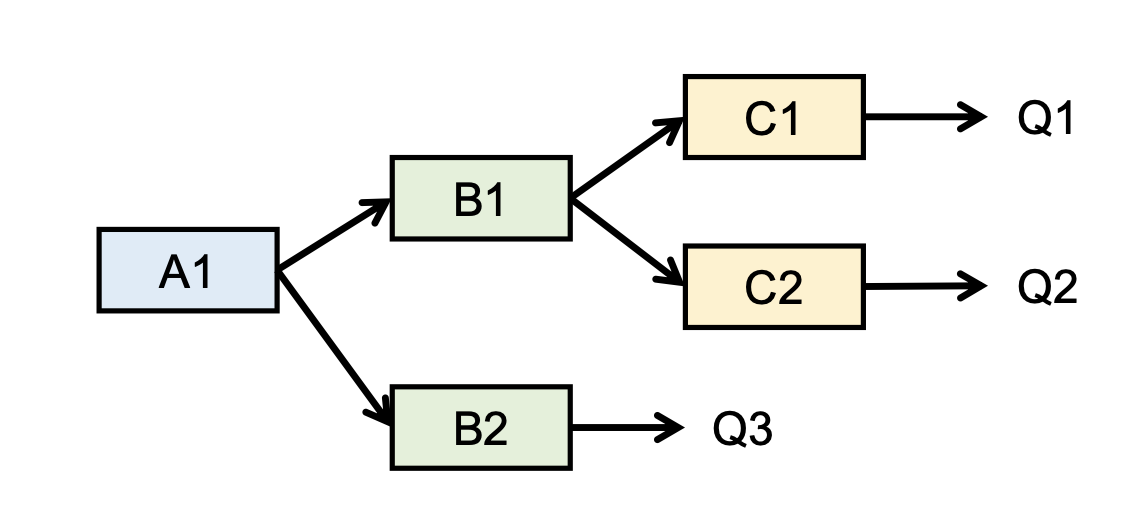
\includegraphics[width=0.8\linewidth]{illustration_images/radix_tree.png}
    \caption{An example of a radix tree from~\cite{MLSYS2025_96894468}, where queries Q1, Q2 share A1, B1 sub-sequences with each other, and only A1 with query Q3.}
    \label{fig:radix_tree_example}
\end{figure}
vLLM~\cite{kwon2023efficient} also implements automatic prefix caching~\cite{vllm_prefix_caching_docs} using a hashing scheme inspired by Merkle trees, as shown in Figure~\ref{fig:vllm_merkle_tree_example}. Each KV-cache block is assigned a hash that depends on both the tokens inside the block and the hash of the preceding prefix block. This effectively forms a chain of hashes representing the entire prefix. If two requests produce the same sequence of hashes, the system can freely reuse the corresponding KV-cache blocks.

\begin{figure}[H]
    \centering
    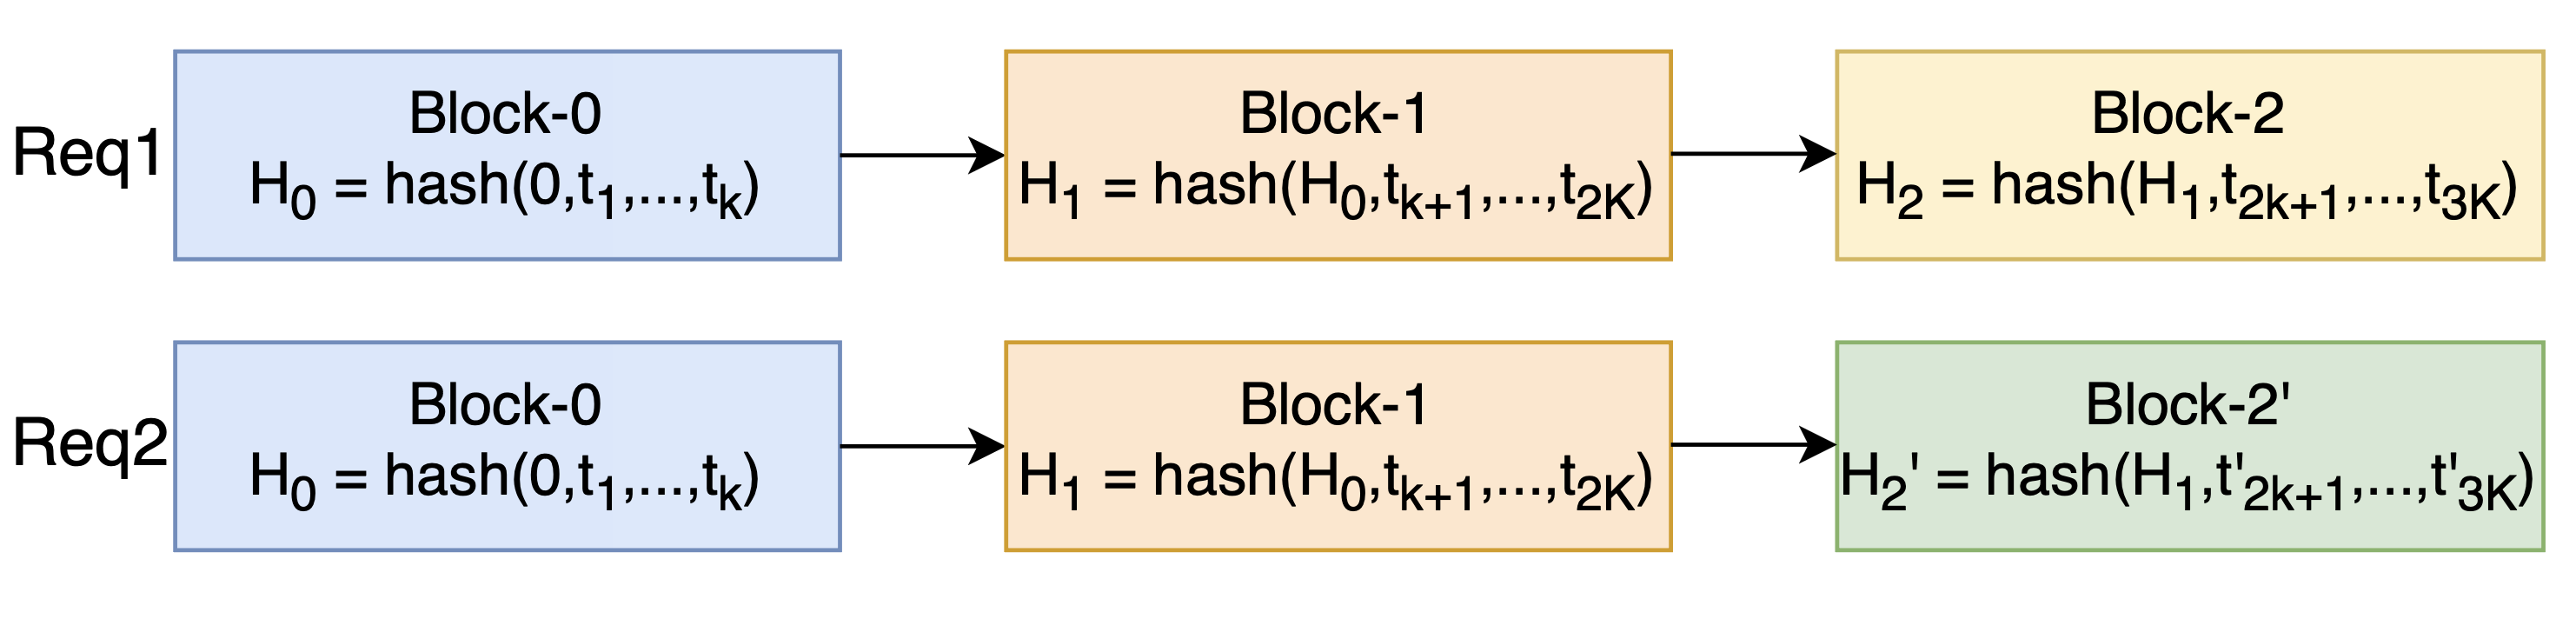
\includegraphics[width=0.8\linewidth]{illustration_images/vllm_merkle_tree.png}
    \caption{An example of vllm Merkle Tree.}
    \label{fig:vllm_merkle_tree_example}
\end{figure}

BatchLLM~\cite{zheng2025batchllmoptimizinglargebatched} extends the idea of prefix sharing to large offline batches, explicitly grouping requests by shared prefixes for global KV cache reuse, then reordering them and applying memory-aware token batching to improve the mix of prefill and decode tokens. BlendServe~\cite{zhao2024blendserveoptimizingofflineinference} similarly leverages a resource-aware prefix tree, but pairs it with a scheduling algorithm that jointly optimizes for both prefix reuse and complementary compute-memory demand balancing. Together, these systems establish that effective prefix sharing requires not just identifying common prefixes but also carefully scheduling the order in which requests are processed to maximize KV cache hit rates and memory efficiency.

\subsection{Prefix-Aware Attention Kernels}
While the systems above handle prefix sharing at the serving and scheduling level, a complementary line of work focuses on exploiting shared prefix structure directly inside the attention kernel, reducing redundant global memory traffic at the GPU execution level. PAT~\cite{yi2025patacceleratingllmdecoding} takes a direct approach by packing queries that share the same prefix into a single CTA, so the shared KV cache is loaded from global memory once and broadcast across all grouped queries. It introduces a pack-forward-merge pipeline with a prefix-aware pack scheduler, multi-tile attention kernels, and multi-stream execution to improve hardware utilization. DEFT~\cite{yao2025deftdecodingflashtreeattention} addresses the same problem in tree-structured decoding by grouping queries according to their shared KV prefixes (KV-guided grouping), ensuring each prefix segment is fetched exactly once; it further introduces Flattened Tree KV Splitting to balance KV partitions across thread blocks for uniform GPU utilization. ChunkAttention~\cite{ye2024chunkattentionefficientselfattentionprefixaware} approaches the problem from a memory layout perspective, storing KV caches in a prefix tree of chunked KV tensors and introducing a two-phase partition kernel, chunk-first and sequence-first, to improve memory locality and parallelism when operating over shared prefix chunks. (\textcolor{red}{improve chunk attention description}) FastTree~\cite{MLSYS2025_96894468} targets radix-tree-structured workloads specifically, grouping queries that share the same tree context to reuse KV cache directly from shared memory, reducing global memory pressure and better utilizing tensor cores. Across all these works, the common insight is that the key to efficient prefix-aware attention lies in restructuring how queries are grouped and how KV data is loaded.

\textcolor{red}{do we need to mention the delta here, or we can skip?}

\section{Motivation}
\label{sec:motivation}
\subsection{Experiment Setup and Overview}
Our central hypothesis is that \textbf{decode-phase} throughput is largely determined by the memory access pattern of the KV cache rather than by compute. In particular, when all the requests in a batch share a common prefix, their attention operations traverse the same KV cache regions at roughly the same time. This aligned access pattern improves spatial and temporal locality in the GPU memory hierarchy, allowing the hardware to better utilize cache capacity and memory bandwidth. Conversely, when requests have heterogeneous prefixes, KV accesses become interleaved across disjoint regions of memory, disrupting locality and reducing effective bandwidth utilization. \textcolor{green}{Another goal which we wish to achieve through our experiments is to evaluate if we can reap locality gains without changing attention kernels.}

To validate this hypothesis, we design a series of controlled experiments that systematically vary (i) the amount of prefix sharing within a batch, (ii) the number of distinct prefix groups, and (iii) the batch size and decode length. Across these experiments, we measure decode throughput and memory behaviour to understand how prefix structure affects inference performance. Each experiment concludes with a takeaway summarizing the key insight.

All experiments use the LLama3-8B \cite{llama3modelcard} model.  Experiments are performed on an RTX6000 Ada Generation GPU \cite{nvidia_rtx6000_datasheet}, equipped with 48GB of GDDR6 memory and a 96MB L2 cache. We use the vLLM \cite{kwon2023efficient} inference engine with a default maximum batch size of 500 unless stated otherwise. We primarily focus on decode-phase throughput, measured in output tokens per second. To isolate decode behaviour, we perform a warm-up run such that all prefix KV caches are resident in GPU memory prior to measurement. This ensures that the per-token compute cost remains constant across experimental settings and that observed differences arise primarily from memory behaviour and batching effects. Later, we also compare end-to-end throughput, which includes the time taken to prefill the queries. For this model, a single 10k-token request generates approximately 1.4GB of KV cache data (across all layers, for both keys and values). Within each layer, KV tensors corresponding to consecutive tokens are stored contiguously in memory. We pick requests from the L-Eval \cite{an2023leval} dataset, and we prune the size of each request as required by the experiment. We use the FlashAttention~\cite{dao2022flashattentionfastmemoryefficientexact} backend throughout all the experiments.


\subsection{Locality and Sharing}
We begin by examining how \textit{prefix heterogeneity} within a batch affects decode throughput.  Prefix heterogeneity refers to the presence of requests with different input prefixes in the same batch.  When requests share the same prefix, they access the same KV cache regions during decode; when prefixes differ, the KV accesses correspond to different memory regions.

To quantify the impact of prefix heterogeneity, we design a controlled experiment with two large system prompts, $A$ and $B$, each of length $10{,}000$ tokens. We form a batch of $500$ requests, where each request consists of either prefix $A$ or $B$, followed by a unique suffix of length $20$ tokens (Figure~\ref{fig:two_fam_vis}). Each request then generates 50 decode tokens. Let $f \in [0,1]$ denote the fraction of requests using prefix $A$. When $f=0$ or $f=1$, the batch is homogeneous, and all $500$ requests share a single prefix. When $0 < f < 1$, two distinct prefix families coexist within the same batch. We do a warmup run before measuring the decode throughput, which ensures that the KV caches corresponding to both the prefix groups are already resident in the GPU memory, and the amount of compute involved is the same across all values of $f$.

Figure~\ref{fig:two_fam_tp} shows decode throughput as a function of $f$. Throughput is maximized when the batch is homogeneous ($f = 0$ or $f = 1$). However, introducing even a single request from the other prefix family causes a sharp degradation. Specifically, at $f = 0.002$ (one request out of $500$), throughput drops by nearly $2\times$. This demonstrates that decode throughput is extremely sensitive to even minimal prefix heterogeneity within a small batch.

\begin{figure}[H]
    \centering
    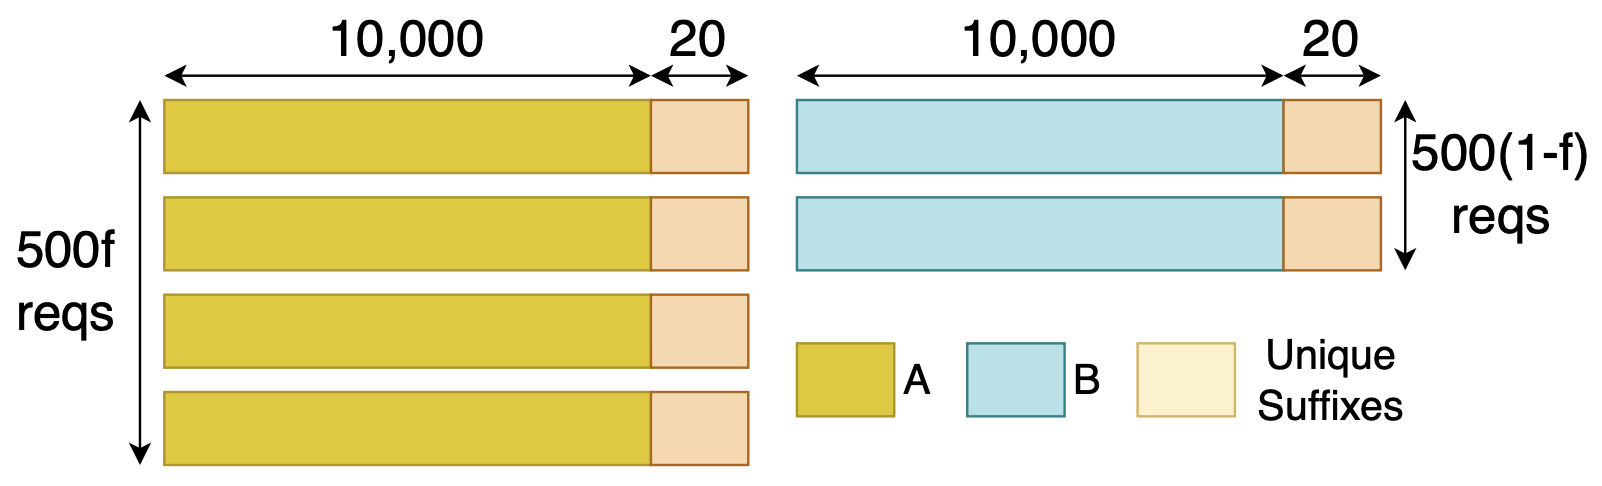
\includegraphics[width=\linewidth]{illustration_images/two_family_experiment.png}
    \caption{Visualization of Heterogeneous Batches}
    \label{fig:two_fam_vis}
\end{figure}
\textcolor{red}{Do we need to mark fractions such as $0.002$ or $0.01$ more clearly in this graph?}

To better understand this effect, we measure mean DRAM activity, defined as the fraction of cycles during which the DRAM pipe is active. As shown in Figure~\ref{fig:two_fam_mean_dram}, homogeneous batches exhibit over $50\%$ higher DRAM activity compared to mixed-prefix settings.

A $10$k-token prefix corresponds to over $1$GB of KV cache data (across all layers). Even with sharing across requests, the active KV working set during decode substantially exceeds the $96$MB L2 cache capacity of the GPU, particularly after accounting for model weights. Thus, decode is fundamentally memory-bound, and only a small portion of the KV cache can reside in L2 at any given time.

\textcolor{red}{present max bandwidth numbers here}

During each decode step, every request attends to its entire prefix. Because the prefix length (10k tokens) dominates both the decode length (50 tokens) and the query length, memory accesses are largely determined by prefix traversal. In the homogeneous case, all requests sweep through the same KV blocks nearly simultaneously. This produces two beneficial effects: (i) \textbf{Spatial Locality:} Sequential traversal of contiguous KV tensors allows the hardware prefetcher to reliably fetch upcoming cache lines from DRAM into L2; (ii) \textbf{Temporal Locality:} Since requests access the same KV regions at roughly the same time, a cache line fetched for one request is likely reused by neighbouring requests before eviction. Together, these effects increase L2 hit rates and sustain high DRAM pipeline utilization, resulting in higher throughput. Since we use a query-centric (FlashAttention) backend, most SMs process queries from the dominant prefix group even when $f = 0.002$. Therefore, we attribute the performance gains primarily to improved L2 cache reuse rather than increased L1 cache locality.

In contrast, when even a small fraction of requests uses a different large prefix, the KV access stream becomes interleaved across two disjoint memory regions. This disrupts prefetcher confidence and weakens spatial locality. More importantly, temporal locality collapses; cache lines fetched for prefix $A$ are unlikely to be reused by prefix $B$ requests before eviction. The result is reduced effective bandwidth utilization and significantly lower throughput.

\textbf{Takeaway 1:} Decode throughput is highest when all requests in a batch share the same prefix, allowing their attention operations to access the same KV cache regions at nearly the same time. Even a single request with a different prefix forces the GPU to interleave accesses across multiple KV regions, breaking cache locality and sharply reducing effective memory bandwidth.

The previous experiment raises a natural follow-up question: \emph{how does throughput change when requests partially share their prefixes rather than being completely identical or completely different?}  Our hypothesis is that if decode performance is primarily determined by KV cache locality, then increasing the amount of shared prefix across requests should progressively improve throughput. Larger shared regions should allow more requests to access the same KV blocks within a short time window, strengthening cache reuse and improving effective memory bandwidth utilization. 

To test this hypothesis, we isolate the effect of prefix sharing by constructing a batch of $100$ requests, each with a total length of $2000$ tokens. In this experiment, every request shares a common prefix of length $2000 \times f$ tokens, where $f \in [0, 1]$. The remaining $2000 \times (1-f)$ tokens are unique to each request, as illustrated in Figure~\ref{fig:frac_share_vis}. As before, a warm-up run ensures that all the $2000$-tokens of each of the $100$ requests are already present in the GPU memory, so that we can attribute the trend in throughput solely to the locality present amongst the requests.

\begin{figure}[H]
\centering
\begin{minipage}{0.48\columnwidth}
    \centering
    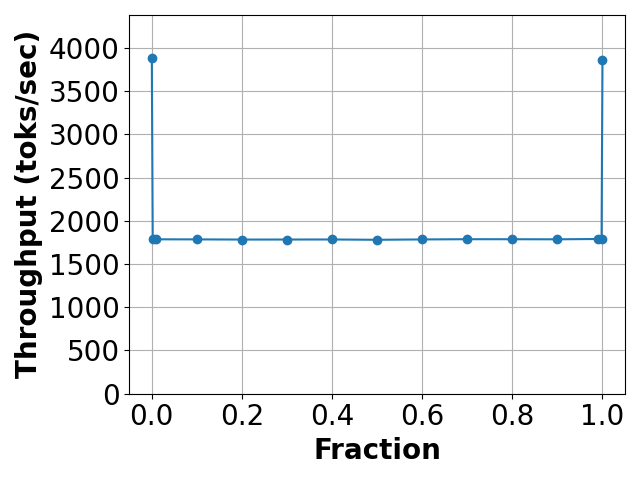
\includegraphics[width=\linewidth]{results/throughput_vs_fraction_two_fam_llama8b.png}
    \caption{Throughput vs Fraction of $A$ prefix requests}
    \label{fig:two_fam_tp}
\end{minipage}
\hfill
\begin{minipage}{0.48\columnwidth}
    \centering
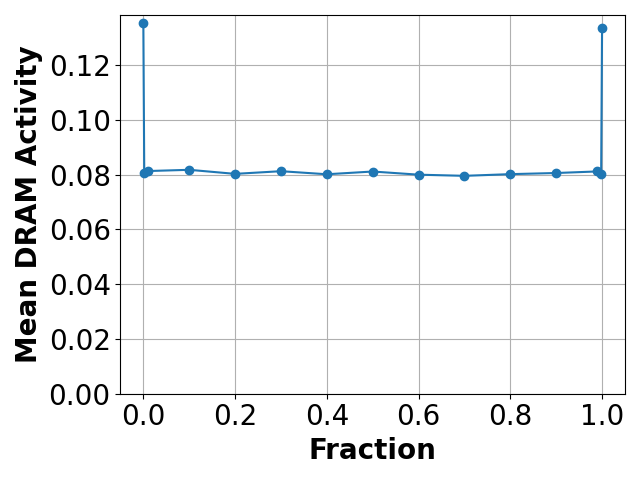
\includegraphics[width=\linewidth]{results/mean_dram_activity_vs_fraction_two_fam_llama8b.png}
\caption{Mean DRAM Activity vs Fraction of $A$ prefix requests}
\label{fig:two_fam_mean_dram}
\end{minipage}
\end{figure}




\begin{figure}[H]
\centering
\begin{minipage}{0.48\columnwidth}
    \centering
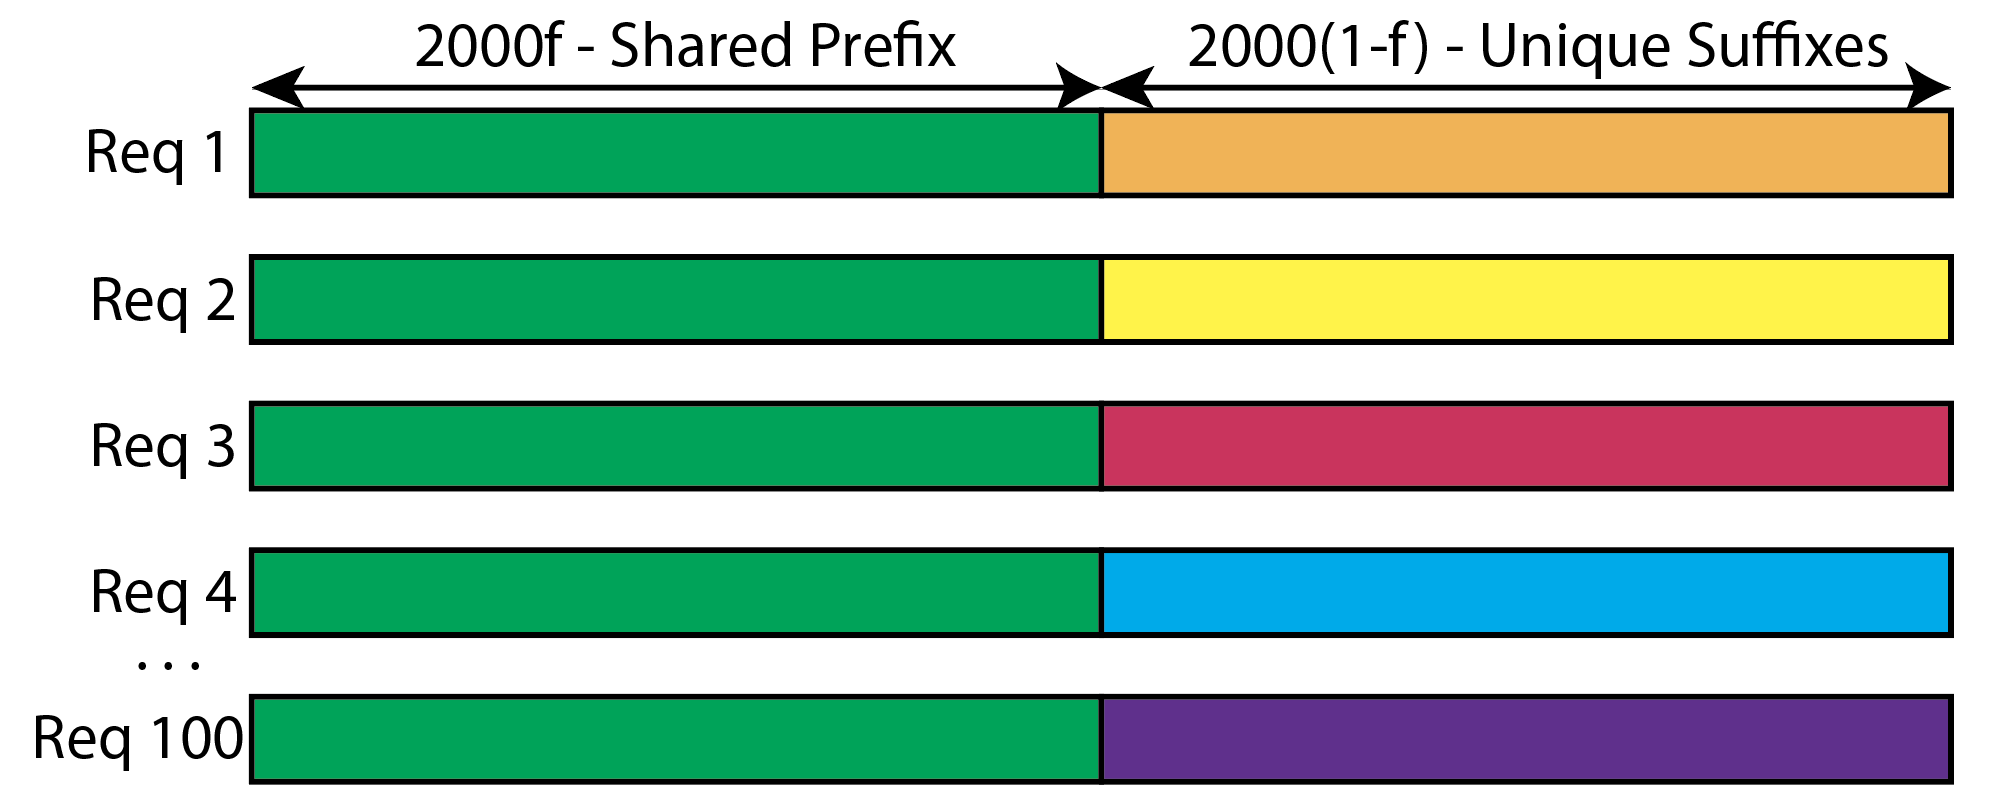
\includegraphics[width=\columnwidth]{illustration_images/fraction_sharing_experiment.png}
\caption{Visualization of $2000\times f$ tokens shared by requests}
\label{fig:frac_share_vis}
\end{minipage}
\hfill
\begin{minipage}{0.48\columnwidth}
    \centering
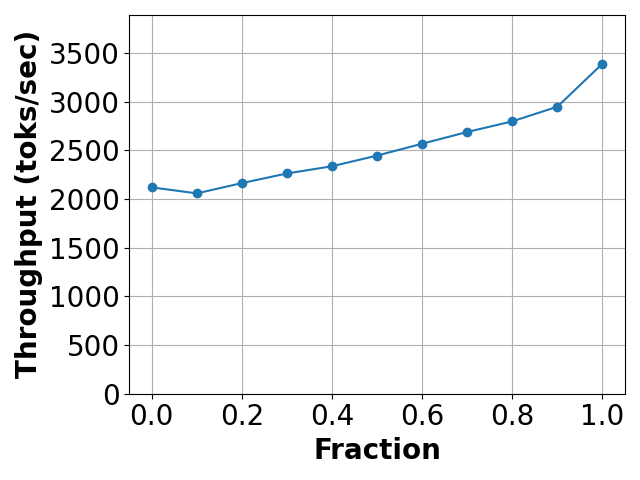
\includegraphics[width=\columnwidth]{results/throughput_vs_fraction_frac_share_llama8b.png}
\caption{Throughput vs Fraction of Sharing}
\label{fig:frac_share_tp}
\end{minipage}
\end{figure}


As shown in  Figure~\ref{fig:frac_share_tp}, there is a smooth increase in throughput with $f$. When there is no shared prefix ($f = 0$), throughput is at its lowest. As sharing increases, throughput improves consistently. When all requests share the entire prefix ($f = 1$), throughput is more than 60\% higher than in the no-sharing case. As $f$ increases, a larger portion of the KV cache becomes common across the batch. Since decode for each token repeatedly sweeps the entire KV cache, the shared region is accessed by multiple requests within a short time window, improving contiguity across memory accesses. Both temporal and spatial locality, therefore, improve with $f$, resulting in improved throughput.

\textbf{Takeaway 2:} Decode throughput increases smoothly with the amount of shared prefix across requests. Greater sharing enlarges the KV regions accessed jointly by the batch, strengthening cache reuse and improving effective memory bandwidth utilization.

The previous experiment varies only the \emph{amount} of sharing while assuming that the shared tokens appear at the beginning of the sequence. This raises a natural question: \emph{does the position of sharing within a sequence also affect decode throughput?} Our hypothesis is that because decode proceeds token by token and all requests traverse their prefixes at the same time, sharing that occurs earlier in the sequence should have a larger impact on locality than sharing that occurs later. Early shared segments allow the batch to access the same KV regions simultaneously, while later divergence breaks this alignment. To test this hypothesis, we design five sharing patterns: complete sharing, no sharing, and sharing with 2, 3, or 4 levels, as illustrated in Figure~\ref{fig:sharing_configurations}. In all configurations, the total sequence length of each request is fixed at $4L$, and only the branching structure differs. We measure decode throughput across these five settings for three values of $L$, as shown in Figure~\ref{fig:tp_vs_l_1_9_11}.

The complete sharing pattern consistently achieves substantially higher throughput than all others. This behavior is expected: full sharing preserves synchronized traversal of the KV cache throughout the entire sequence, maximizing both temporal and spatial locality.

A more subtle observation is that configurations with 2, 3, and 4 levels exhibit similar throughput across different values of $L$, despite differing branching patterns. This can be explained by the timing of memory accesses during decode. Requests within a batch issue memory accesses roughly simultaneously. During the initial shared segment of length $L$, all configurations behave identically; every request accesses the same KV region, fully exploiting locality. Once branching occurs, the batch becomes heterogeneous, and locality degrades. However, as we will show next, throughput is highly sensitive to the presence of heterogeneity but comparatively less sensitive to the exact number of distinct prefix groups once heterogeneity is introduced.  Whether the batch ultimately splits into two, four, or eight groups in later segments has only a limited additional impact since synchronized reuse has already been disrupted. Moreover, as expected, no sharing pattern achieves the lowest throughput of all.

\textbf{Takeaway 4:} Because decode-phase memory accesses from all sequences occur roughly together, the amount of sharing at the beginning of the sequence is the primary determinant of locality and throughput.



\begin{figure}[H]
    \centering
    \captionsetup[subfigure]{labelformat=simple}
    \renewcommand\thesubfigure{(\alph{subfigure})}
    \begin{subfigure}{0.25\columnwidth}
        \centering
        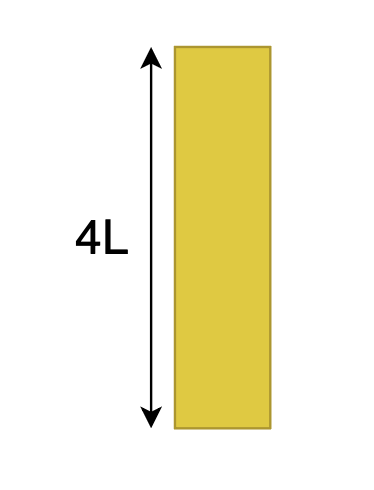
\includegraphics[width=\linewidth]{illustration_images/vis_complete_sharing.png}
        \caption{Complete sharing}
        \label{fig:vis_complete_sharing}
    \end{subfigure}
    \hfill
    \begin{subfigure}{0.35\columnwidth}
        \centering
        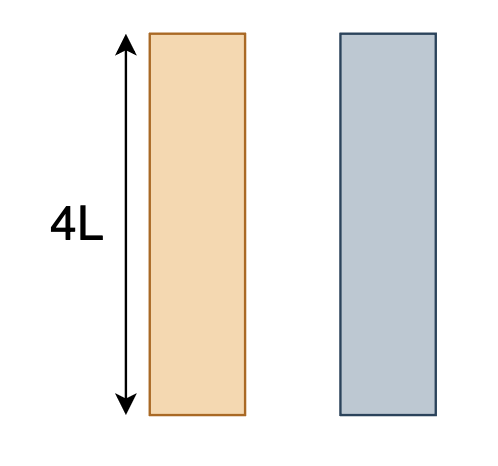
\includegraphics[width=\linewidth]{illustration_images/vis_no_sharing.png}
        \caption{No sharing}
        \label{fig:vis_no_sharing}
    \end{subfigure}
    \hfill
    \begin{subfigure}{0.35\columnwidth}
        \centering
        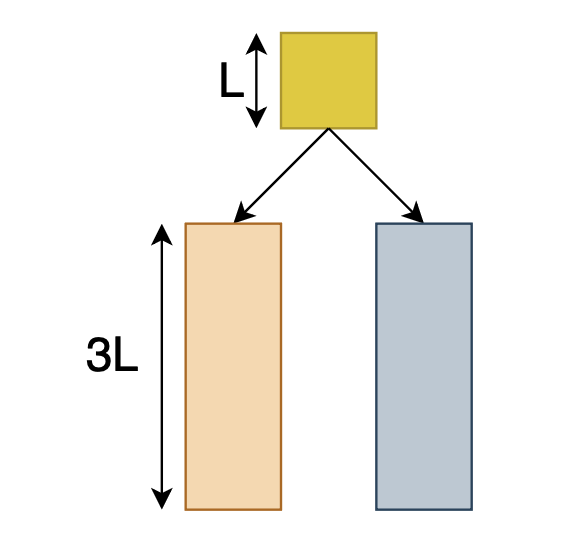
\includegraphics[width=\linewidth]{illustration_images/vis_2_levels.png}
        \caption{2 Levels}
        \label{fig:2_levels}
    \end{subfigure}

    \vspace{0.5cm}

    \begin{subfigure}{0.40\columnwidth}
        \centering
        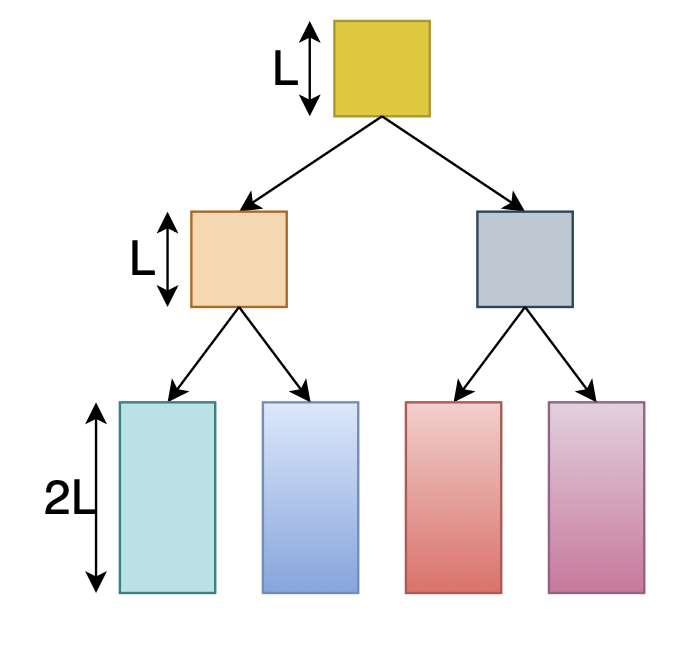
\includegraphics[width=\linewidth]{illustration_images/vis_3_levels.png}
        \caption{3 Levels}
        \label{fig:3_levels}
    \end{subfigure}
    \hfill
    \begin{subfigure}{0.58\columnwidth}
        \centering
        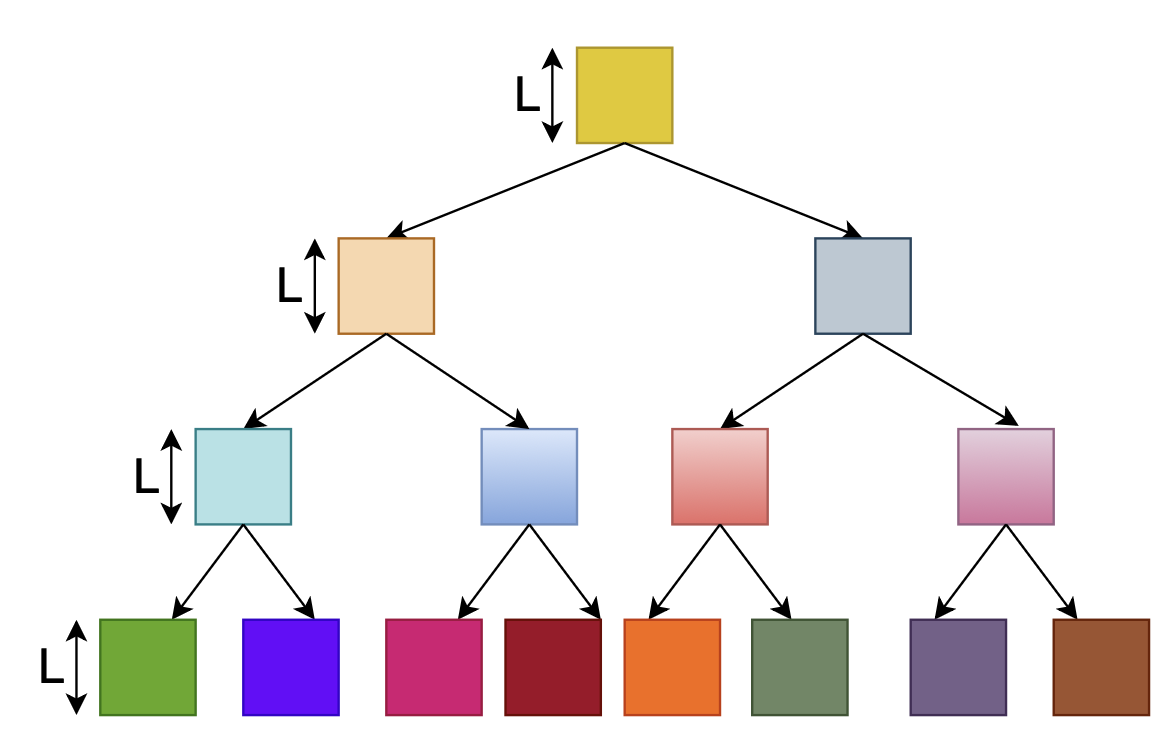
\includegraphics[width=\linewidth]{illustration_images/vis_4_levels.png}
        \caption{4 Levels}
        \label{fig:4_levels}
    \end{subfigure}

    \caption{Visualization for different sharing patterns}
    \label{fig:sharing_configurations}
\end{figure}


\begin{figure}[H]
\centering
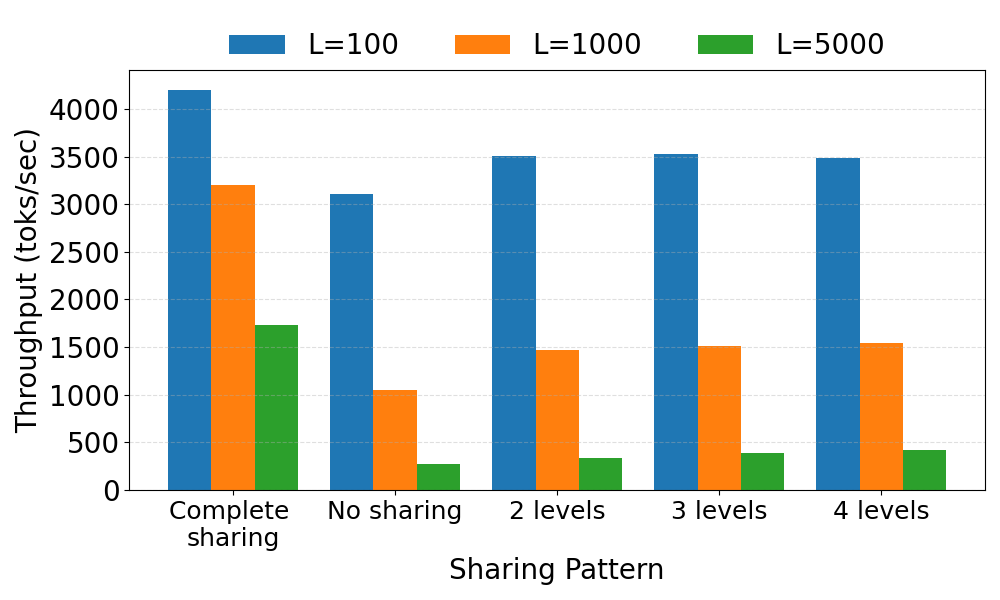
\includegraphics[width=\columnwidth]{results/tp_different_modes_sharing_at_top.png}
\caption{Throughput vs sharing patterns for different sequence lengths}
\label{fig:tp_vs_l_1_9_11}
\end{figure}

The previous experiments examine how prefix sharing affects decode throughput when the KV caches of all active requests fit within GPU memory. However, in some practical serving workloads, a system may need to handle many distinct prefixes simultaneously. This raises another important question: \emph{what happens when the number of distinct prefixes becomes large enough that their KV caches cannot all reside in GPU memory?} Our hypothesis is that when the number of active prefixes grows beyond the available GPU memory capacity, the system will be forced to evict KV cache blocks. These evictions require recomputation when the corresponding requests resume their decode phases, leading to reduced throughput and smaller effective batch sizes.

To study this effect, we construct an experiment with $N$ different shared prefixes $P_1, P_2 \dots P_N$, each of length $5000$ tokens. We create batches such that an equal number of requests corresponds to each prefix. Figure~\ref{fig:hbm_evic_tp_bs} shows the resulting throughput and average batch size as $N$ increases. As observed earlier, throughput drops when moving from $N = 1$ to $N = 2$, primarily due to reduced temporal and spatial locality. From $N = 2$ to $N = 20$, throughput remains relatively stable, indicating that locality degradation alone does not worsen performance beyond the initial heterogeneity. However, there is a sharp decline in throughput from $N = 20$ to $N = 50$. This drop occurs because the available GPU memory is no longer sufficient to hold the KV caches for all active prefixes simultaneously. This leads to frequent KV cache evictions and recomputations. The effect is also reflected in the reduced average batch size for $N = 50$ and $N = 100$, as the system cannot admit new requests due to limited GPU memory capacity. This phenomenon has also been explored in prior work~\cite{zheng2025batchllmoptimizinglargebatched,pang2025optimizingllminferencethroughput}, which highlights the impact of KV cache capacity constraints on inference throughput.

\textbf{Takeaway 4:} Beyond cache locality, the number of simultaneously active prefixes also affects performance through GPU memory capacity limits. Prefix-aware scheduling can mitigate KV cache evictions and improve throughput.

\begin{figure}[H]
\centering
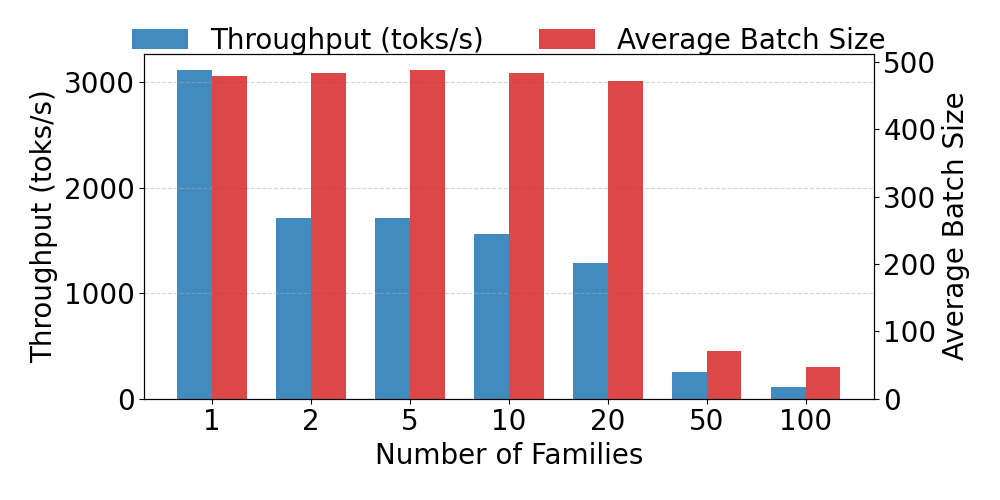
\includegraphics[width=\columnwidth]{results/hbm_evictions_fcfs_throughput_vs_batchsize_dual_axis.png}
\caption{Throughput and Average Batch Size vs Number of Prefix Groups}
\label{fig:hbm_evic_tp_bs}
\end{figure}


\subsection{Effect of Batch Size on Decode Throughput}
The previous experiments show that decode throughput is strongly influenced by prefix structure, which determines how effectively requests can reuse KV cache data. However, prefix sharing is only one factor that affects performance. Another important parameter in LLM serving systems is the \emph{batch size}, which determines how much parallel work is issued to the GPU during each decode step.

Our hypothesis is that increasing batch size should initially improve throughput by better utilizing GPU compute units, particularly tensor cores. However, once compute resources are saturated, decode performance should become limited by memory bandwidth, since each additional request increases KV cache traffic.

To study this effect, we evaluate decode phase throughput as a function of batch size. In this experiment, all the requests start from one of the 5 large prefixes of length $2000$ tokens each.  As shown in Figure~\ref{fig:batch_size_tp_motivation}, throughput increases with batch size due to improved tensor core utilization (Figure~\ref{fig:batch_size_tenso}). However, another point worth noting is that beyond a certain batch size, once the GPU’s compute units are already highly utilized, the throughput curve largely flattens. The mean SM Occupancy is shown in Figure~\ref{fig:batch_size_smocc} (\textcolor{red}{currently linked to appendix plot, can remove this}).

\textbf{Takeaway 5:} We should aim to increase the batch size to better utilize GPU compute, but only up to the point when the tensor core utilization saturates, after which decode performance is no longer limited by arithmetic throughput but by KV cache movement between HBM and on-chip caches. At that stage, simply adding more requests to the batch does not yield proportional gains because memory becomes the bottleneck.

\begin{figure}[H]
\centering
\begin{minipage}{0.48\columnwidth}
\centering
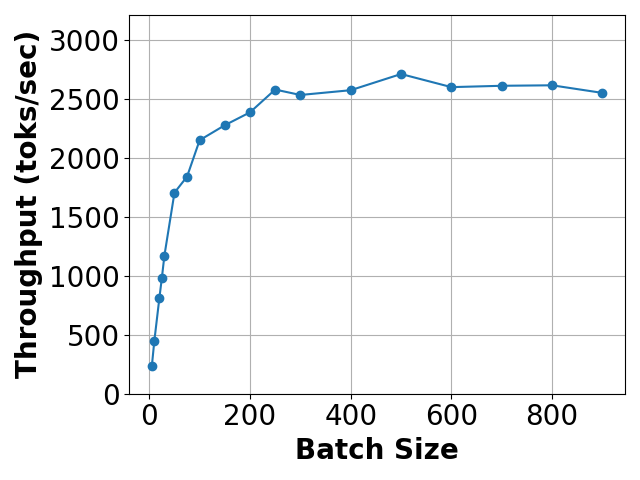
\includegraphics[width=\columnwidth]{results/throughput_vs_batch_size_llama8b.png}
\caption{Throughput vs Batch Size}
\label{fig:batch_size_tp_motivation}
\end{minipage}
\hfill
\begin{minipage}{0.48\columnwidth}
\centering
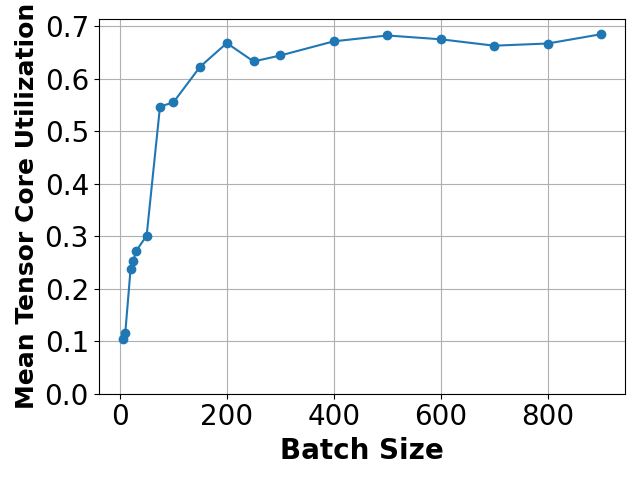
\includegraphics[width=\columnwidth]{results/mean_tenso_vs_batch_size_llama8b.png}
\caption{Tensor Core Utilization vs Batch Size}
\label{fig:batch_size_tenso}
\end{minipage}
\end{figure}


The previous experiment examined how batch size affects decode throughput under a fixed prefix structure. In practice, however, LLM serving workloads involve both \emph{prefill} and \emph{decode} phases. These two stages stress different system resources: prefill is primarily compute-intensive, while decode is largely memory-bound due to repeated traversal of the KV cache. Consequently, the benefits of prefix locality observed in earlier experiments may manifest differently when considering end-to-end execution.

Our first hypothesis is that the benefits of prefix locality should become increasingly pronounced as the decode length grows. Prefill is largely a write-heavy workload that constructs the KV cache once, while decode repeatedly reads the entire prefix at every generation step. As the number of decode tokens increases, these repeated KV sweeps amplify the impact of memory locality.

Moreover, there exists a trade-off between large heterogeneous batches and smaller prefix-homogeneous batches. Large heterogeneous batches maximize tensor core utilization, while homogeneous batches preserve aligned traversal of the KV cache during decode.

To evaluate these hypotheses, we measure end-to-end throughput, including both prefill and decode phases. Unlike previous decode-only experiments, we do not perform a warmup run; thus, prefix computation and KV cache construction are included in the reported throughput. We consider a workload consisting of eight distinct prefix groups, each containing 100 requests (800 total). We evaluate several batching strategies: (i) a single heterogeneous batch of 800 requests spanning all eight families; (ii) two batches of 400 requests covering four families each; (iii) four batches of 200 requests covering two families each; (iv) eight batches of 100 requests, each homogeneous; (v) sixteen batches of 50 requests, each homogeneous; and (vi) thirty-two batches of 25 requests, each homogeneous. We further vary the number of decode tokens to study how the prefill–decode balance influences performance.

Figure~\ref{fig:prefill_decode_tp_batch_config_decode} shows throughput across these configurations. When the decode length is small, throughput is largely influenced by prefill computation. In this regime, larger heterogeneous batches tend to perform well because they maximize tensor core utilization and arithmetic intensity during the prefix processing stage. As we progressively split the large 1×800 batch into 2×400 and 4×200 configurations, throughput decreases slightly, reflecting reduced compute efficiency from smaller batch sizes. In this setting, the benefits of memory locality are not yet dominant enough to compensate for the loss in arithmetic utilization.

However, as we increase the number of decode tokens, there is a shift in the performance trend. Decode requires each request to repeatedly sweep its entire KV cache. When batches are heterogeneous, these sweeps interleave across disjoint memory regions, weakening spatial and temporal locality. As a result, memory accesses become fragmented and effective bandwidth utilization decreases. In contrast, once we transition to fully homogeneous batches (8$\times$100), throughput increases significantly, even though each batch is smaller than the earlier configurations. This improvement arises because all requests within a batch now share the same prefix, restoring synchronized traversal of the KV cache and strengthening both spatial and temporal locality.

Interestingly, even the 16$\times$50 configuration, which further reduces batch size but remains homogeneous, continues to outperform the single large heterogeneous batch (1$\times$800) when the decode length is sufficiently large. This demonstrates that the locality benefits from prefix alignment can outweigh the loss in tensor core utilization. Only when batches become too small (32$\times$25) does throughput begin to decline again. At that point, reduced arithmetic intensity and lower tensor core occupancy dominate, and the compute under-utilization can no longer be compensated by improved memory alignment.

The impact of decode length further illustrates this trade-off. When the number of decode tokens is small (e.g., 10 tokens), a homogeneous batch of size $50$ does not outperform a heterogeneous batch of size 800, since the workload remains largely dominated by prefill computation and compute efficiency plays a larger role. However, when we increase the decode length to 100 tokens, the homogeneous 50-request batch begins to surpass the large heterogeneous batch. This occurs because each additional decode step requires another full sweep of the KV cache, allowing the benefits of aligned memory access patterns to accumulate over time. As decode length increases, execution becomes increasingly memory-bound, and the advantage of prefix-homogeneous batching becomes more pronounced.

Overall, these results highlight a fundamental balance between compute utilization and memory locality. Large heterogeneous batches maximize tensor core usage but fragment KV access patterns. Moderately sized homogeneous batches preserve aligned traversal of the KV cache and can achieve higher effective throughput when decode dominates execution. The optimal operating point lies where compute resources remain well utilized while memory access patterns remain synchronized across requests.

\textbf{Takeaway 6:} Under end-to-end execution, it is often beneficial to process requests in prefix-homogeneous batches, even if this slightly reduces batch size. As the number of decode tokens increases, repeated KV cache sweeps amplify the benefits of memory locality, allowing moderately sized homogeneous batches to outperform larger heterogeneous batches. However, this benefit holds only up to a point: when batches become too small, reduced tensor core utilization and lower arithmetic intensity lead to underutilized compute, causing throughput to decline.
\begin{figure}[H]
\centering
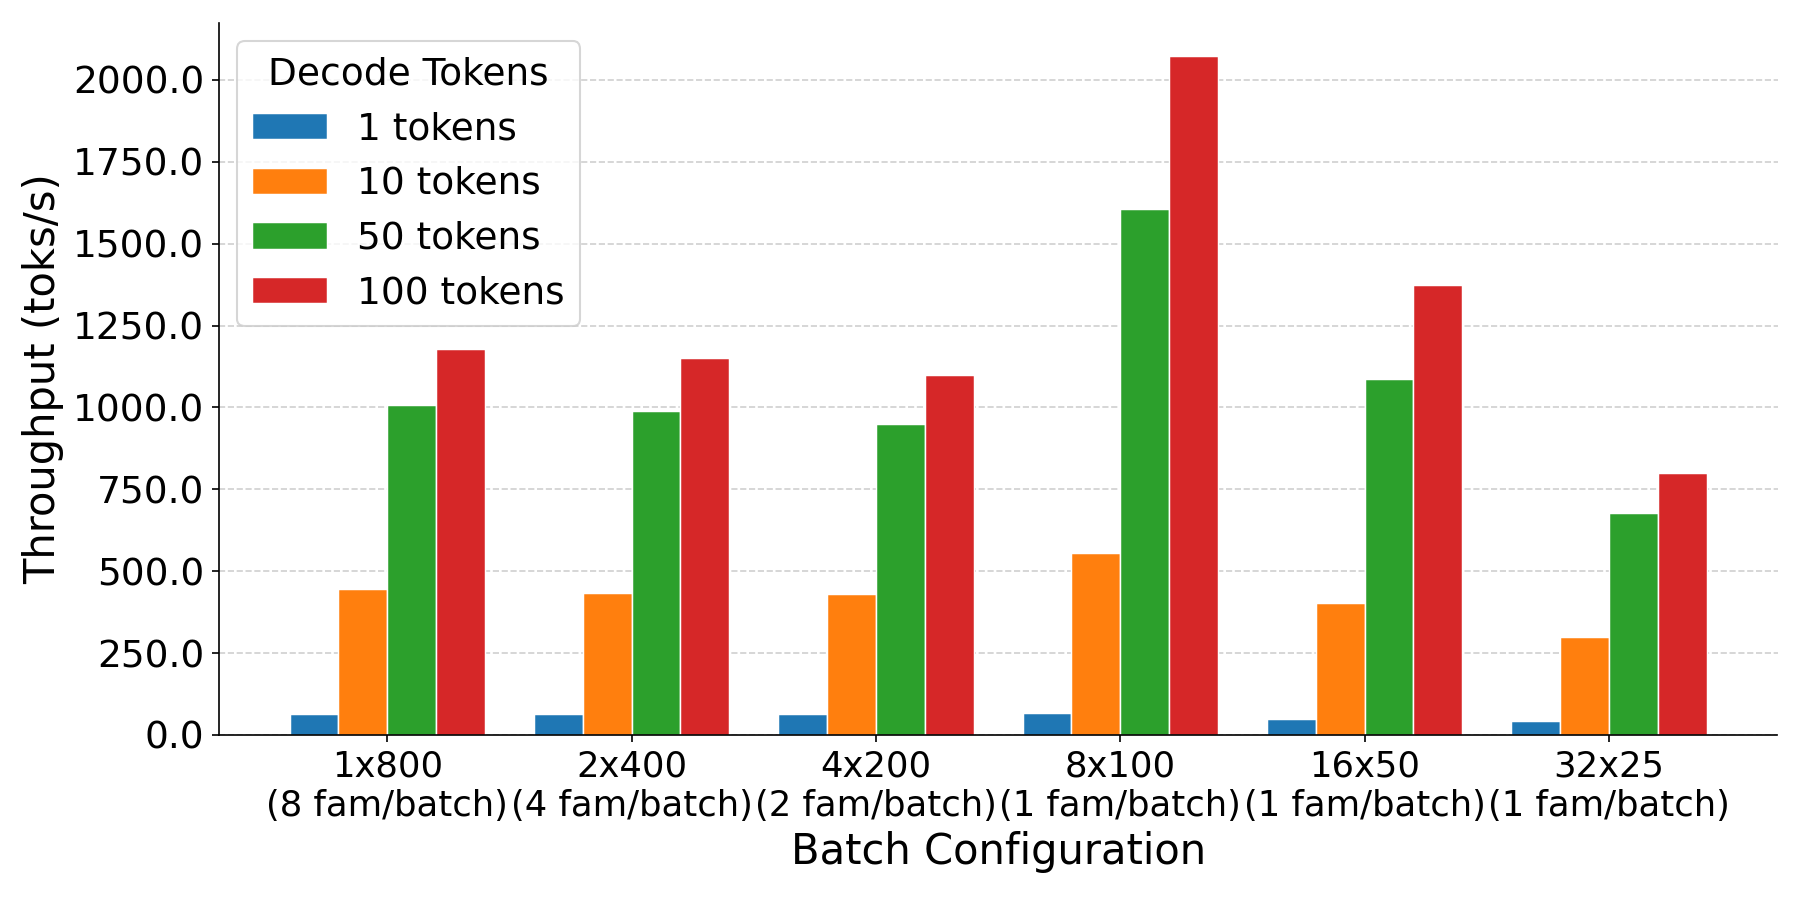
\includegraphics[width=\columnwidth]{results/prefill_decode_homo_hetero_grouped_throughput.png}
\caption{Throughput vs Batch Configurations for varying number of decode tokens}
\label{fig:prefill_decode_tp_batch_config_decode}
\end{figure}


\subsection{Overhead of dynamic prefix detection}
So far, we have analyzed how the prefix sharing structure and batch size affect the overall inference throughput. Next, we plan to study how the state-of-the-art inference engines identify prefix sharing and what the overall cost involved in doing this is. Although existing inference engines such as SGLang \cite{zheng2024sglangefficientexecutionstructured} and BatchLLM \cite{zheng2025batchllmoptimizinglargebatched} do not consider making the batch prefix-homogeneous, they still attempt to detect prefix sharing using radix trees to schedule requests in an order that minimizes KV cache recomputations. In SGLang, two radix-tree-aware scheduling policies are proposed. The first, \emph{Longest Prefix Match (LPM)}, prioritizes requests whose input prefixes match the longest cached prefixes \textcolor{red}{a better definition needed here?}. The second, \emph{DFS-Weight}, performs a depth-first traversal of the radix tree and prioritizes branches that have more active requests. To understand the overhead of these scheduling policies, we implemented a radix-tree-based scheduler inside vLLM and measured its CPU cost. We constructed a workload of 2000 requests, each with a 10k-token prefix, and compared the CPU time spent on scheduling against the total execution time. We also compared these results with an idealized policy in which the user directly provides prefix group identifiers, eliminating the need for any dynamic prefix discovery. \textcolor{red}{describe prefix aware attention here, after reading through, and check if it matches on what we have implemented}

Table~\ref{tab:cost_schedulers} shows the results. SGLang’s LPM and DFS-Weight policies incur 78.24 and 89.06 seconds of CPU time, respectively, on the same order as the GPU computation. Our radix-tree implementation in vLLM reduces this overhead somewhat (57.53 seconds), but the cost remains substantial. In contrast, when prefix group identifiers are provided explicitly, the CPU overhead drops to just 0.03 seconds.

There is a structural reason for this gap: radix trees require token-by-token comparisons during insertion, dynamic node splitting when partial matches occur, and the maintenance of shared paths as requests arrive and complete. Scheduling decisions further require repeated traversals of the tree. With long prompts and high concurrency, these operations accumulate significant constant-factor overhead. 

\textbf{Takeaway 7:} Existing approaches introduce significant CPU overhead while detecting prefix sharing, which is at times even comparable to the GPU execution time. 
\begin{table}[t]
\centering
\small
\resizebox{\columnwidth}{!}{\begin{tabular}{lcccc}
\toprule
\textbf{Policy} & \textbf{Batch Time (s)} & \textbf{Exec (s)} & \textbf{Throughput} & \textbf{TC Util.} \\
\midrule
vLLM FCFS & 3e-6 & 229.36 & 436.25 & 0.67 \\
vLLM User IDs & 0.03 & 105.43 & 948.54 & 0.336 \\
vLLM RadixTree & 62.95 & 139.33 & 717.35 & 0.20 \\
SGLANG DFS-W & 92.15 & 177.78 & 562.61 & 0.22 \\
SGLANG LPM & 46.62 & 149.27 & 669.92 & 0.26 \\
\bottomrule
\end{tabular}}
\caption{Comparison of scheduling policies}
\label{tab:cost_schedulers}
\end{table}

\textcolor{red}{add prefix aware attention tree after reading the paper and implementing their idea}

\textcolor{red}{remove vllm radix tree as it has our own optimizations, or we can keep it still?}

\textcolor{red}{batchLLM avoids this cost by shifting to offline serving, similar to blendserve.}




\section{Design and Implementation}
\label{sec:design}

\begin{figure*}[t]
\centering
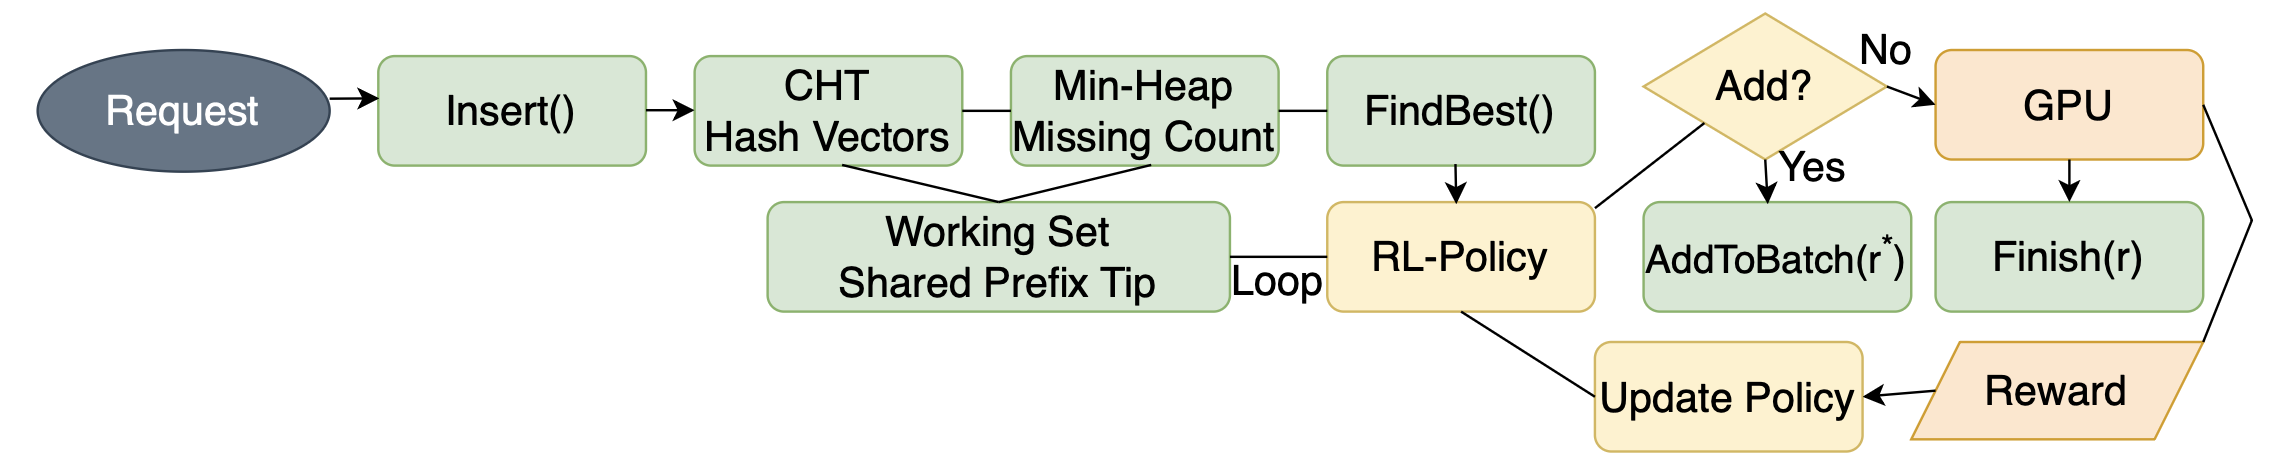
\includegraphics[width=2\columnwidth]{illustration_images/pipeline.png}
\caption{Entire Pipeline}
\label{fig:pipeline}
\end{figure*}

As shown in \S\ref{sec:motivation}, during the decode phase, memory accesses from different requests in a batch are issued almost at the same time. When all requests pass through the same KV cache in the same order, the accesses become nicely sequential, which helps the hardware prefetcher and improves effective DRAM bandwidth utilization. In this setting, as we demonstrated earlier, both temporal and spatial locality naturally emerge. However, this benefit only holds when sharing is universal across the batch. As soon as sharing becomes partial, even slightly, the reuse opportunity drops sharply. Similarly, grouping requests by prefix not only improves locality but also reduces KV cache eviction pressure, thereby preventing expensive recomputation.

\paragraph{Insight 1.} The joint objective that emerges is to keep the GPU busy while also preserving shared-prefix locality for as long as possible. A simple way to think about this is through the pair: \textbf{(Batch size, Shared prefix tokens common to all requests)}. Increasing batch size improves compute utilization. Increasing the number of shared prefix tokens across all active requests strengthens temporal and spatial locality. The goal, therefore, is not merely to build large batches, but to build large, \emph{homogeneous} batches.

\paragraph{Challenge 1.} At each step of batch formation, where we continuously add requests from the waiting queue into the running scheduler batch, there exists a trade-off between adding a new request to increase GPU utilization and maintaining temporal and spatial locality over a longer shared prefix. This trade-off is sensitive to the interplay between the GPU's compute capability and memory bandwidth, making it difficult to resolve with a fixed heuristic across different kinds of GPUs. In particular, it is unclear when to fall back from a homogeneous batch (all requests sharing a long prefix) to a heterogeneous one (mixed prefixes), especially when insufficient homogeneous requests are available in the queue. 

\paragraph{Key Idea 1.} We propose learning a reinforcement learning (RL) policy for the scheduler that adaptively resolves this trade-off at runtime, guided by the observed reward.

\paragraph{Insight 2.} Beyond scheduling, efficiently identifying which requests share a common prefix is a critical bottleneck in itself. Existing approaches to prefix detection incur significant CPU overhead, causing stalls during inference; particularly as sequence lengths grow to thousands of tokens.

\paragraph{Challenge 2.} Designing a data structure that supports fast, low-overhead prefix identification at scale is non-trivial. The structure must handle long sequences efficiently, support dynamic insertion and lookup, and impose minimal CPU cost so as not to bottleneck the inference pipeline.

\paragraph{Key Idea 2.} We introduce \emph{Chunked Hash Tree}, a data structure that detects shared prefixes with substantially lower CPU overhead than existing methods and scales well to longer sequences.



\subsection{System Overview} 
\label{sec:system_overview}
Figure~\ref{fig:pipeline} illustrates the overall pipeline of our scheduling system. The goal of the scheduler is to construct batches that both keep the GPU well utilized and preserve spatial-temporal locality for the KV cache. To achieve this, our design combines two main components:
(i) a lightweight prefix-tracking data structure called \emph{Chunked Hash Tree (CHT)} and
(ii) a learning-based policy that decides when batch construction should stop.

\paragraph{Request model.} We consider an inference server that continuously receives decoding requests. Each request consists of a prompt, which is a sequence of input tokens, followed by autoregressive decoding. At any point in time, a request falls into one of these three states: 
(i) \emph{waiting} requests that have not yet been scheduled,
(ii) \emph{active} requests that are currently part of the decoding batch, and
(iii) \emph{finished} requests whose decoding has been completed.

The scheduler operates in repeated decoding steps. During each step, it incrementally constructs a batch by selecting requests from the waiting queue and activating them. Once the batch is finalized, it is executed for one decoding iteration on the GPU.

\paragraph{Prefix-aware request selection.} The first challenge is identifying which waiting request should be added next to the batch. Ideally, we want to add requests whose prefixes overlap with those of the already active requests, since this increases temporal and spatial locality. To support this efficiently, we introduce \emph{Chunked Hash Tree}. Instead of comparing token sequences directly, each request is represented using a compact vector of cumulative prefix hashes computed at fixed token intervals. These hashes allow the scheduler to quickly detect shared prefixes across requests. The CHT maintains a working set that represents the prefixes currently referenced by active requests and tracks how much prefix overlap each waiting request has with this working set. Using this information, the scheduler can efficiently identify the waiting request that maximizes our joint objective function.

\paragraph{Batch construction loop.} Using the CHT, the scheduler repeatedly retrieves the best candidate request from the waiting queue (the one with the highest prefix overlap) and considers adding it to the current batch. Each candidate provides useful statistics, such as the current batch size, the shared-prefix length across all active requests before and after the addition, and the number of waiting requests that could benefit from the same prefix. At this point, the scheduler must decide whether to add the request or stop building the batch. Adding more requests improves GPU utilization but may reduce prefix locality if the shared prefix becomes smaller.

\paragraph{Learning when to stop.} We formulate this decision as a learning problem. The scheduler observes a state that summarizes the current batch size and prefix-sharing statistics, and a reinforcement learning policy chooses between two actions: \textsc{Add} the candidate request to the batch or \textsc{Stop} and dispatch the batch for execution. After the batch is executed, the system observes the resulting performance (e.g., throughput) and uses it as feedback to update the policy. Over time, the policy learns how to balance GPU utilization and prefix locality for different workload conditions.

\paragraph{End-to-end flow.} Putting everything together, the pipeline works as follows. Incoming requests are first inserted into the CHT, where their prefix hashes are computed and indexed. During batch construction, the scheduler repeatedly calls \textsc{FindBest} to retrieve the best candidate request based on prefix overlap. The reinforcement learning policy then decides whether to activate the request and add it to the batch or to stop. Once the batch is finalized, it is dispatched for execution on the GPU. The observed throughput is then used to update the policy for future scheduling decisions. 

The following subsections describe the Chunked Hash Tree data structure in detail and then present the batching and reinforcement learning policies built on top of it.

\subsection{Chunked Hash Tree}
\textcolor{red}{a better name, without a tree, for uniqueness. Do we need to make it a separate section?}

\textcolor{red}{starting with a brief overview}

\textcolor{red}{need to mention that implemented in C++ (can do so in the section integration with vllm)}

\begin{figure*}[t]
\centering
\begin{subfigure}{0.32\textwidth}
    \centering
    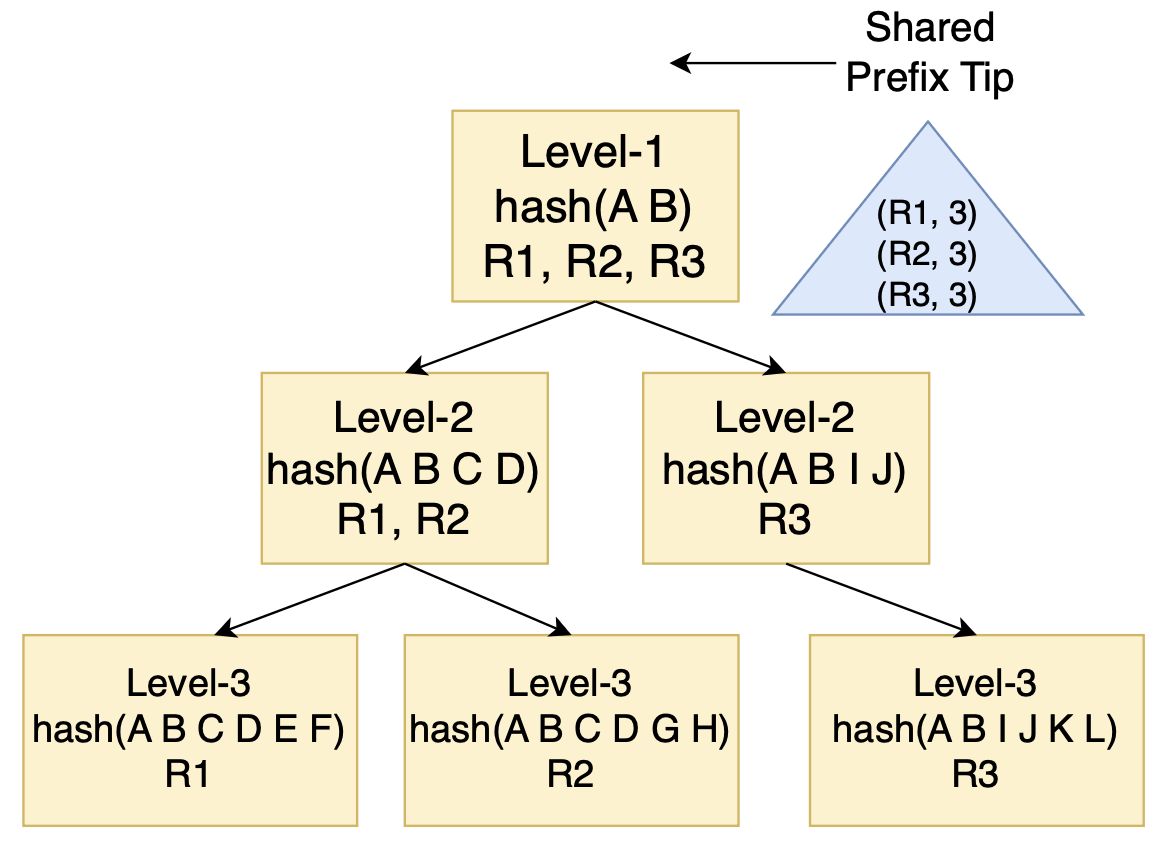
\includegraphics[width=\linewidth]{illustration_images/chunked_hash_tree_insertion.png}
    \caption{}
    \label{fig:chunked_hash_tree_insertion}
\end{subfigure}
\hfill
\begin{subfigure}{0.32\textwidth}
    \centering
    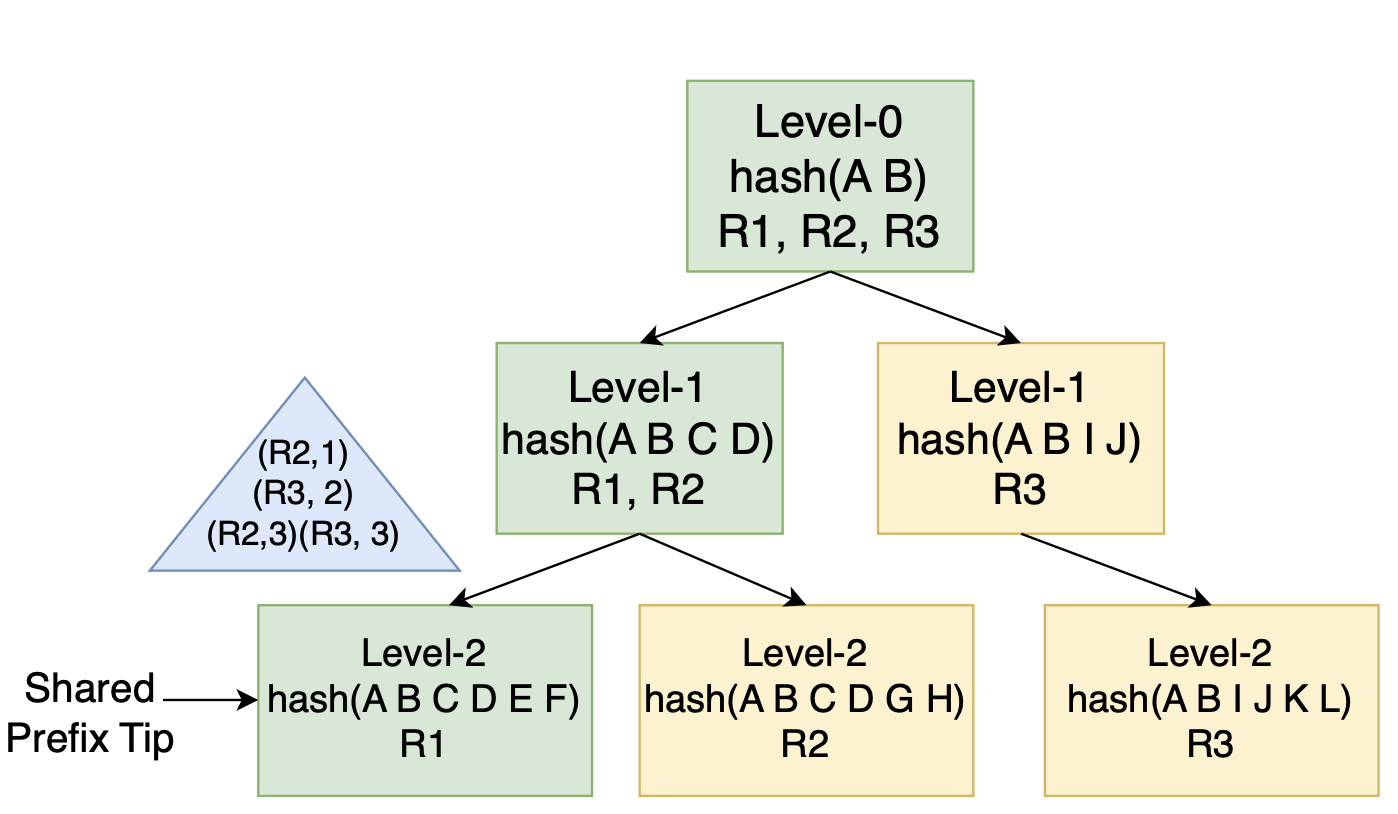
\includegraphics[width=\linewidth]{illustration_images/chunked_hash_tree_activation.png}
    \caption{}
    \label{fig:chunked_hash_tree_activation}
\end{subfigure}
\hfill
\begin{subfigure}{0.32\textwidth}
    \centering
    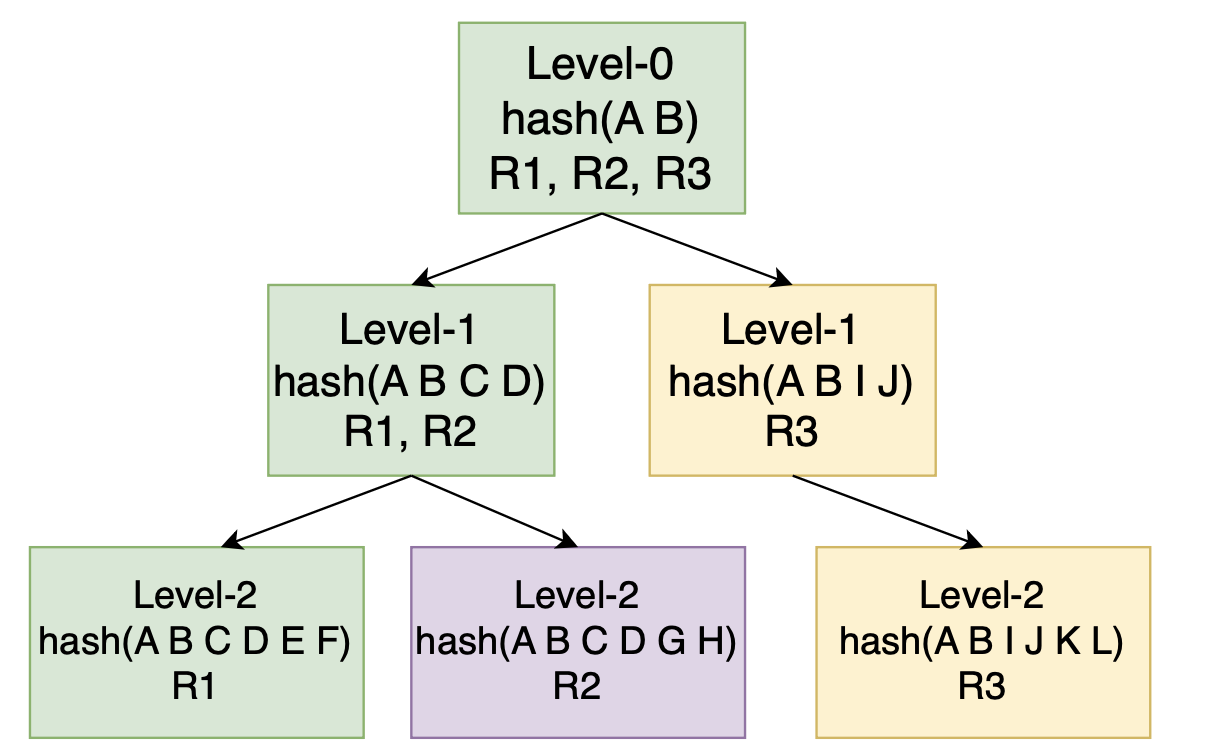
\includegraphics[width=\linewidth]{illustration_images/chunked_hash_tree_find_best_request.png}
    \caption{}
    \label{fig:chunked_hash_tree_find_best_request}
\end{subfigure}

\caption{An example of chunked hash tree workflow which shows insertion, activation and best request selection. Consider 3 requests $R_1, R_2, R_3$ each with 6 tokens. With a chunk size of 2, each request will get divided into 3 levels, as shown in~\ref{fig:chunked_hash_tree_insertion}. Next, we add $R_1$ to the active decoding batch, this makes the shared prefix chain include all its nodes, which are marked as green in ~\ref{fig:chunked_hash_tree_activation}. Now, we wish to find the next candidate request which can be added to the running batch. We have two options $R_2$ and $R_3$. Since, $R_2$ has the max overlap with the current shared prefix chain, we prefer it over $R_3$, as shown in~\ref{fig:chunked_hash_tree_find_best_request}.}
\label{fig:chunked_hash_tree_workflow}
\end{figure*}


\subsubsection*{Motivation and Design Evolution} The scheduler repeatedly needs to answer a simple question: among all waiting requests, which one shares the largest prefix with the currently active batch? Requests that share longer prefixes will lead to higher temporal and spatial locality. Since scheduling decisions occur frequently and the waiting queue may contain thousands of requests with long prompts, detecting prefix overlap must be extremely fast and impose minimal CPU overhead.

Modern inference systems already exploit prefix sharing for KV-cache reuse. As shown in \S\ref{sec:background}, vLLM~\cite{kwon2023efficient} uses Merkle Trees, while SGLang~\cite{zheng2024sglangefficientexecutionstructured} and BatchLLM~\cite{zheng2025batchllmoptimizinglargebatched} use radix trees to detect prefix sharing. Our scheduler, however, has a different objective: we do not need to store or manage KV-cache blocks; instead, we only need a lightweight way to estimate how much prefix overlap exists between requests so that we can select the best request to add to the batch. While a radix tree precisely captures prefix sharing, it incurs significant overhead; every insertion may trigger node splitting, and finding the best matching waiting request requires a DFS traversal that is $O(W)$ in the worst case, where $W$ is the number of waiting requests. For a scheduler making frequent decisions over thousands of long-prompt requests, that is quite expensive. Similarly, Merkle-style hash chains introduce unnecessary sequential dependencies during hash computation and expose more structure than the scheduler actually requires.

We instead want a structure centered around a \emph{working set}: the set of prefix chunks currently held by active requests; so that we can directly ask: ``which waiting request has the most overlap with the already running batch?'' This reframes the problem from tree traversal to set intersection. To that end, rather than maintaining a strict hash chain, we divide the token sequence into fixed-size chunks and compute prefix hashes at chunk boundaries. An additional advantage of this design is that hash computation can be naturally batched and parallelized. Because chunks are processed independently, their hash contributions can be computed separately and later combined to obtain the cumulative prefix hashes. This pattern is similar in spirit to techniques such as online softmax, where partial statistics are computed over blocks and then merged to produce the final result. In contrast, Merkle-style hash chains require sequential computation because each hash depends on the previous one.

The simplest realization is to represent each request as a set of hashed prefix chunks, maintain the working set explicitly, and, on each scheduling decision, scan all waiting requests and count how many of their chunks appear in the working set. The request with the highest overlap wins. This is correct and easy to implement, but finding the best request is $O(W \cdot C)$ --- linear in the number of waiting requests times chunks per request, since we rescan everything on every call.

We can avoid rescanning by maintaining a \emph{missing count} per waiting request: the number of its chunks that are absent from the working set. This count only needs to change when the working set itself changes, i.e., upon activation or completion of a request. Instead of recomputing overlaps from scratch, we propagate small delta updates. Finding the best request then becomes a linear scan over waiting requests to find the minimum missing count — $O(W)$.

To eliminate the linear scan, we maintain a min-heap ordered by missing count. When a chunk enters or leaves the working set, we update the missing counts of affected waiting requests and push new entries to the heap. However, in-place heap updates are expensive, so we use \emph{lazy deletion}: push a new entry with the updated count, and skip stale entries (where the heap's recorded count differs from the current missing cache) when popping. This reduces the complexity to $O(\log W)$ amortized, while keeping activation and completion costs proportional only to the number of \emph{affected} waiting requests per chunk—typically far smaller than $W$.

The resulting structure, which we call the \emph{Chunked Hash Tree} (CHT), is a scheduling data structure that maximizes KV-cache prefix reuse across concurrent inference requests. We first describe how requests are represented as hash vectors, then introduce the data structures that track the scheduler state, and finally walk through each operation in turn.


\subsubsection*{Hash Computation}
Before a request can be inserted into the scheduler, its token sequence must be converted into a compact representation that captures the prefix-sharing structure.  As shown in Figure~\ref{fig:chunked_hash_tree_prefix_representation}, given a request with a token sequence $T = (t_1, t_2, \dots, t_N)$, we partition $T$ into non-overlapping chunks of size $K$ (e.g., $K = 50$). For each chunk boundary $\ell = 1, \dots C$ where $C = \lceil N/K \rceil$, we compute a \emph{cumulative prefix hash} at each boundary\\ $h_\ell = \mathrm{hash}(t_1, t_2, \dots, t_{\min(\ell K,\, N}), \quad \ell = 1, \dots, C$.

Because the hash is cumulative, two requests share the same $h_\ell$ if and only if their first $\ell K$ tokens are identical, which is precisely the condition under which their KV-cache prefixes can be shared. Each request $r$ is therefore represented as an ordered hash vector $H_r = (h_1^r, h_2^r, \dots, h_C^r)$.

Algorithm~\ref{alg:compute_hashes} details the hash computation. We use an incremental xxHash-64 state so that each token is processed exactly once, making the total cost $O(N)$ regardless of the number of chunked boundaries.

\begin{algorithm}[H]
\caption{$\textsc{ComputeHashes}(T, K)$}
\label{alg:compute_hashes}
\begin{algorithmic}[1]
\Require Token sequence $T = (t_1, \dots, t_N)$; chunk size $K$
\Ensure Cumulative prefix-hash vector $H = (h_1, \dots, h_C)$
\State $H \gets []$;\quad $C \gets \lceil N / K \rceil$
\State Initialise incremental \textsc{xxHash-64} state $s$
\For{$i \gets 1$ \textbf{to} $N$}
  \State Feed $t_i$ into $s$
  \If{$i \bmod K = 0$ \textbf{or} $i = N$}
    \State $H.\textsc{Append}(\textsc{Digest}(s))$
  \EndIf
\EndFor
\State \Return $H$
\end{algorithmic}
\end{algorithm}

\begin{figure}[H]
\centering
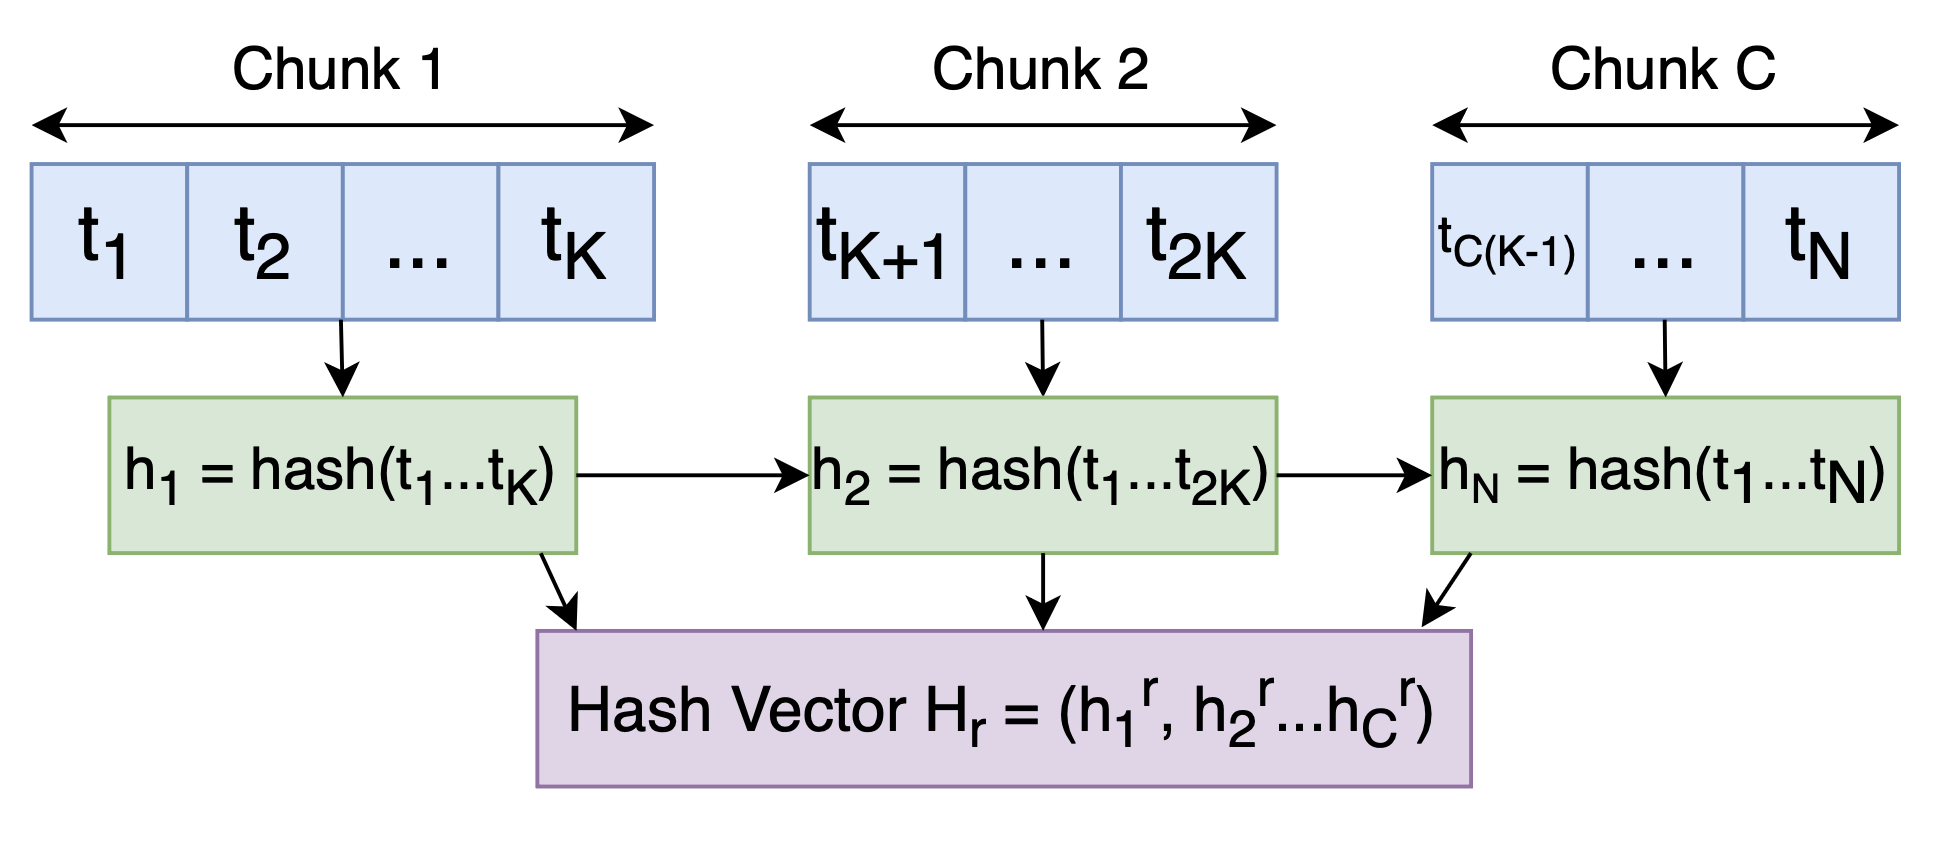
\includegraphics[width=\columnwidth]{illustration_images/chunked_hash_tree_prefix_representation.png}
\caption{Hash Computation in Chunked Hash Tree}
\label{fig:chunked_hash_tree_prefix_representation}
\end{figure}

\subsubsection*{Data Structures}
The CHT maintains the following components that together capture the full scheduler state:

\paragraph{Hash vectors.} A map from request ID to its cumulative prefix-hash vector $H_r = (h_1^r, \dots, h_C^r)$ is stored for every active and waiting request.

\paragraph{Reference counts.} \texttt{ref} maps each $h$ to the number of currently \emph{active} requests that contain that hash in their hash vectors. 

\paragraph{Working set.} \texttt{working\_set} is the set of hashes that belong to at least one \emph{active} request. A hash is in the working set if and only if its reference count is greater than zero.

\paragraph{Missing cache.} \texttt{miss} maps each \emph{waiting} request $r$ to an integer $m_r$, defined as the number of hashes in $H_r$ that are \emph{not} currently in the working set. Intuitively, $m_r$ counts how many of $r$'s prefix chunks would need to be freshly computed (i.e., are not already cached by the active batch). A request with $m_r = 0$ has its entire prefix covered by the current active batch and is therefore the most preferable candidate to admit next.

\paragraph{Waiting heap.} \texttt{waiting\_heap} is a min-heap of $(m_r, r)$ pairs, ordered by missing count $m_r$. It enables $O(\log W)$ retrieval of the waiting request with the smallest missing count, where $W$ is the number of waiting requests.

\paragraph{Reverse index.} \texttt{waiting} maps each hash $h$ to the set of waiting requests whose hash vector contains $h$, enabling $O(1)$ updates to \texttt{miss} when the working set changes.

\paragraph{Shared prefix chain.} \texttt{shared\_prefix\_chain} is a vector $P = (p_1, \dots, p_L)$ recording the longest common hash prefix shared by all currently active requests. $P$ is maintained incrementally rather than recomputed from scratch for every event, keeping the amortized cost low. 


\subsubsection*{Request Insertion (Algorithm~\ref{alg:insert})}
$\textsc{Insert}$ is called the moment a new request arrives at the scheduler. It computes $H_r$ via $\textsc{ComputeHashes}$, stores the hash vector, and for each hash $h \in H_r$, registers $r$ in the reverse index $\mathit{waiting}[h]$. Crucially, it also computes the initial missing count $m_r$: the number of hashes in $H_r$ not yet present in the working set. This count is stored in $\mathit{miss}[r]$ and the pair $(m_r, r)$ is pushed onto the waiting heap. No reference counts are modified at this stage; that happens only when the request is activated.

\begin{algorithm}[H]
\caption{$\textsc{Insert}(r, T)$}
\label{alg:insert}
\begin{algorithmic}[1]
\Require Request $r$; token sequence $T$; working set $\mathit{working\_set}$; reverse index $\mathit{waiting}$; min-heap $\mathit{waiting\_heap}$
\Ensure $r$ registered and ready for scheduling
\State $H_r \gets \textsc{ComputeHashes}(T, K)$
\State $\mathit{request\_hashes}[r] \gets H_r$
\State $m_r \gets 0$
\State $\mathit{waiting\_requests} \gets \mathit{waiting\_requests} \cup \{r\}$
\For{$\ell \gets 1$ \textbf{to} $|H_r|$}
  \If{$h_\ell^r \notin \mathit{working\_set}$}
    \State $m_r \gets m_r + 1$
  \EndIf
  \State $\mathit{waiting}[h_\ell^r] \gets \mathit{waiting}[h_\ell^r] \cup \{r\}$
\EndFor
\State $\mathit{miss}[r] \gets m_r$
\State $\mathit{waiting\_heap}.\textsc{Push}(m_r,\; r)$
\end{algorithmic}
\end{algorithm}

\paragraph{Activation (Algorithm~\ref{alg:activate}).} 
$\textsc{Activate}$ is called when the scheduler moves a request from the waiting queue into the active decoding batch. For each hash $h$ in $H_r$, if $h$ transitions from absent to present in the working set (i.e., its reference count goes from 0 to 1), then $h$ is added to the working set and all waiting requests that contain $h$ have their missing count decremented by one; updated pairs are pushed onto the heap. This eager propagation keeps $\mathit{miss}$ accurate for all waiting requests without requiring a full rescan. The shared prefix chain is then updated incrementally via $\textsc{UpdateChainOnActivate}$ (Algorithm~\ref{alg:update_chain_activate}).

\begin{algorithm}[H]
\caption{$\textsc{Activate}(r)$}
\label{alg:activate}
\begin{algorithmic}[1]
\Require Request $r$ with hash vector $H_r$; ref counts $\mathrm{ref}$; working set $\mathit{working\_set}$; reverse index $\mathit{waiting}$; missing cache $\mathit{miss}$; min-heap $\mathit{waiting\_heap}$
\Ensure Updated $\mathrm{ref}$, $\mathit{working\_set}$, $\mathit{miss}$; updated shared prefix chain
\State $\mathit{waiting\_requests} \gets \mathit{waiting\_requests} \setminus \{r\}$;
\State       $\mathit{active} \gets \mathit{active} \cup \{r\}$
\State $\mathit{added} \gets 0$
\For{$\ell \gets 1$ \textbf{to} $|H_r|$}
  \If{$\mathrm{ref}[h_\ell^r] = 0$}
  \Comment{$h_\ell^r$ newly enters working set}
  \State $\mathit{working\_set} \gets \mathit{working\_set} \cup \{h_\ell^r\}$
  \For{$w \in \mathit{waiting}[h_\ell^r]$}
      \If{$w \notin \mathit{active}$ \textbf{and} $w \in \mathit{miss}$}
        \State $\mathit{miss}[w] \gets \mathit{miss}[w] - 1$
        \State $\mathit{waiting\_heap}.\textsc{Push}(\mathit{miss}[w],\; w)$
      \EndIf
    \EndFor
    \State $\mathit{added} \gets \mathit{added} + 1$
  \EndIf
  \State $\mathrm{ref}[h_\ell^r] \gets \mathrm{ref}[h_\ell^r] + 1$
\EndFor
\State $\textsc{UpdateChainOnActivate}(r)$
\State \Return $(\mathit{added},\; |H_r|)$
\end{algorithmic}
\end{algorithm}

\paragraph{Updating the shared prefix chain on activation (Algorithm~\ref{alg:update_chain_activate}).}
It is called at the end of every $\textsc{Activate}$ after $r$ has been added to the active set. It keeps the shared prefix chain consistent without recomputing it from scratch. Because adding a new request can only \emph{shorten} the common prefix (never lengthen it), we must find the longest prefix of the current chain $P$ that $H_r$ also satisfies.

As described before, each hash $h_\ell$ is produced by a cumulative (prefix) hasher: $h_\ell$ is the digest of all tokens from position $1$ through $\ell \cdot C$, where $C$ is the chunk size. Consequently, if two hash vectors agree at level $\ell$, they necessarily agree at every level $1, \ldots, \ell-1$ as well, because those earlier digests are sub-sequences of the same cumulative stream. Formally, we define the predicate $\mathcal{M}(\ell) \;=\; \bigl[h_\ell^r = p_\ell\bigr]$. The cumulative property guarantees that $\mathcal{M}$ is \emph{monotone decreasing} on the index set $\{1, \dots, \min(L, |H_r|)\}$: once $\mathcal{M}(\ell)$ is false for some $\ell^*$, it is false for all $\ell > \ell^*$. This monotone structure is exactly the condition required for binary search to be correct: we seek the largest $k$ such that $\mathcal{M}(k)$ is true, and binary search finds it in $O(\log \min(L, |H_r|))$ comparisons rather than the $O(\min(L, |H_r|))$ required by a linear scan.

\begin{algorithm}[H]
\caption{$\textsc{UpdateChainOnActivate}(r)$}
\label{alg:update_chain_activate}
\begin{algorithmic}[1]
\Require Request $r$ with hash vector $H_r$; current shared chain $P$ of length $L$; active set $\mathit{active}$
\Ensure $P$ reflects the longest common prefix of all active requests
\If{$|\mathit{active}| = 1$}
    \Comment{$r$ is the only active request}
    \State $P \gets H_r$;\quad $L \gets |H_r|$
    \State \Return
\EndIf
\State $L \gets \textsc{BinarySearch}\!\left(H_r,\, P,\, \min(L,\, |H_r|)\right)$
\Comment{largest $k$ s.t.\ $h_k^r = p_k$}
\State Truncate $P$ to its first $L$ entries
\end{algorithmic}
\end{algorithm}

\paragraph{Completion (Algorithm~\ref{alg:finish}).} $\textsc{Finish}$ is called when the model has generated the final token for request $r$, and the request is removed from the active batch. For each hash $h$ in $H_r$, its reference count is decremented; if it reaches zero, $h$ is evicted from the working set, and all waiting requests containing $h$ have their missing count incremented by one, with updated pairs pushed onto the heap. The shared prefix chain is then updated via $\textsc{UpdateChainOnFinish}$, since removing a request can only lengthen the common prefix.


\begin{algorithm}[H]
\caption{$\textsc{Finish}(r)$}
\label{alg:finish}
\begin{algorithmic}[1]
\Require Request $r$ with hash vector $H_r$; ref counts $\mathrm{ref}$; working set $\mathit{working\_set}$; reverse index $\mathit{waiting}$; missing cache $\mathit{miss}$; min-heap $\mathit{waiting\_heap}$
\Ensure Updated $\mathrm{ref}$, $\mathit{working\_set}$, $\mathit{miss}$; reverse index cleaned; updated shared prefix chain
\State $\mathit{active} \gets \mathit{active} \setminus \{r\}$
\State $\mathit{evicted} \gets 0$
\For{$\ell \gets 1$ \textbf{to} $|H_r|$}
  \State $\mathrm{ref}[h_\ell^r] \gets \mathrm{ref}[h_\ell^r] - 1$
   \If{$\mathrm{ref}[h_\ell^r] = 0$}
   \State $\mathit{working\_set} \gets \mathit{working\_set} \setminus \{h_\ell^r\}$
    \For{$w \in \mathit{waiting}[h_\ell^r]$}
      \If{$w \notin \mathit{active}$ \textbf{and} $w \in \mathit{miss}$}
        \State $\mathit{miss}[w] \gets \mathit{miss}[w] + 1$
        \State $\mathit{waiting\_heap}.\textsc{Push}(\mathit{miss}[w],\; w)$
      \EndIf
    \EndFor
    \State $\mathit{evicted} \gets \mathit{evicted} + 1$
  \EndIf
\EndFor
\State $\textsc{UpdateChainOnFinish}(r)$
\State $\textsc{Remove}(r)$
  \Comment{cleans $\mathit{waiting}$ index and $\mathit{request\_hashes}$}
\State \Return $(\mathit{evicted},\; |H_r|)$
\end{algorithmic}
\end{algorithm}

\paragraph{Updating the shared prefix chain on completion (Algorithm~\ref{alg:update_chain_finish})}
It is called inside $\textsc{Finish}$, \emph{before} $r$'s hash vector is erased, after $r$ has been removed from the active set. Removing a request can only \emph{extend} the common prefix. We therefore try to grow the chain level by level beyond its current length by checking whether all remaining active requests agree on each successive hash. Two special cases are handled up front: if no requests remain, the chain is cleared; if exactly one request remains, the chain is set to its full hash vector.

\begin{algorithm}[H]
\caption{$\textsc{UpdateChainOnFinish}(r)$}
\label{alg:update_chain_finish}
\begin{algorithmic}[1]
\Require Active set $\mathit{active}$ (already excludes $r$); current shared chain $P$ of length $L$; hash vectors $\mathit{request\_hashes}$
\Ensure $P$ extended as far as all remaining active requests agree
\If{$\mathit{active} = \emptyset$}
\State $P \gets []$;\quad $L \gets 0$;\quad \Return
\EndIf
\If{$|\mathit{active}| = 1$}
  \State $\textsc{RecomputeChain}()$;\quad \Return
  \Comment{sets $P$ to the sole remaining request's full hash vector}
\EndIf
\State $M \gets \min_{q \in \mathit{active}} |H_q|$
  \Comment{maximum possible extension}
\For{$\ell \gets L + 1$ \textbf{to} $M$}
  \State $h^* \gets h_\ell^{q_0}$ for an arbitrary $q_0 \in \mathit{active}$
  \If{$\forall\, q \in \mathit{active} : h_\ell^q = h^*$}
    \State $P.\textsc{Append}(h^*)$;\quad $L \gets L + 1$
  \Else
    \State \textbf{break}
  \EndIf
\EndFor
\end{algorithmic}
\end{algorithm}
 




\subsubsection*{Finding the Best Request (Algorithm~\ref{alg:find_best})}
$\textsc{FindBest}$ is called by the batch-construction loop whenever the scheduler needs to select the next candidate request to admit. The key insight is that the best candidate is the waiting request whose prefix chunks are \emph{most covered} by the current active batch, i.e., the one with the smallest missing count $m_r$. The algorithm extracts the minimum-missing-count entry from the waiting heap, skipping stale entries (those whose recorded missing count no longer matches $\mathit{miss}$ due to lazy deletion). Three auxiliary statistics are then computed to guide the caller's admission decision: 
(i) $\mathit{chunks\_before}$, the shared prefix chain length before the candidate is admitted; 
(ii) $\mathit{chunks\_after}$, the chain length that would result after admitting the candidate, computed by comparing $H_{r^*}$ with $P$; and 
(iii) $\mathit{peers}$, the number of other waiting requests sharing the prefix up to level $\mathit{chunks\_after}$, indicating the future benefit that the admission would unlock.

The result is cached and reused on repeated calls until the working set or waiting queue changes, avoiding redundant heap traversals.

\begin{algorithm}[H]
\caption{$\textsc{FindBest}()$}
\label{alg:find_best}
\begin{algorithmic}[1]
\Require Min-heap $\mathit{waiting\_heap}$ of $(m_r, r)$ pairs; missing cache $\mathit{miss}$; active set $\mathit{active}$; shared chain $P$ of length $L$
\Ensure $(r^*,\;\mathit{chunks\_before},\;\mathit{chunks\_after},\;\mathit{peers})$ or $\bot$ if the waiting queue is empty
\If{$\mathit{waiting\_requests} = \emptyset$}\ \Return $\bot$
\EndIf
\If{$\mathit{cache\_valid}$}\ \Return $\mathit{cached\_result}$
\EndIf
\While{$\mathit{waiting\_heap} \neq \emptyset$}
\State $(m, r) \gets \mathit{waiting\_heap}.\textsc{Pop}()$
  \If{$r \in \mathit{active}$}\ \textbf{continue}
    \Comment{already activated}
  \EndIf
  \If{$r \notin \mathit{miss}$}\ \textbf{continue} \Comment{request no longer exists}
  \EndIf
  \If{$\mathit{miss}[r] \neq m$}\ \textbf{continue}
    \Comment{stale heap entry}
  \EndIf
  \State $r^* \gets r$
  \State $\mathit{chunks\_before} \gets L$
  \State $\mathit{chunks\_after} \gets \textsc{ChainLengthWith}(r^*)$
    \Comment{compare $H_{r^*}$ with $P$}
  \State $\mathit{peers} \gets \textsc{WaitersAtLevel}(\mathit{chunks\_after})$
  \State $\mathit{waiting\_heap}.\textsc{Push}(m, r^*)$
    \Comment{restore entry for future calls}
  \State Cache and \Return $(r^*,\;\mathit{chunks\_before},\;\mathit{chunks\_after},\;\mathit{peers})$
\EndWhile
\State \Return $\bot$
\end{algorithmic}
\end{algorithm}


Figure~\ref{fig:chunked_hash_tree_workflow} shows a worked example of insertion,
activation, and best-request selection. Figure~\ref{fig:shared_prefix_chain_workflow} shows how the shared prefix chain shrinks and extends upon activation and completion of requests.


\begin{figure*}[t]
\centering
\begin{subfigure}{0.24\textwidth}
    \centering
    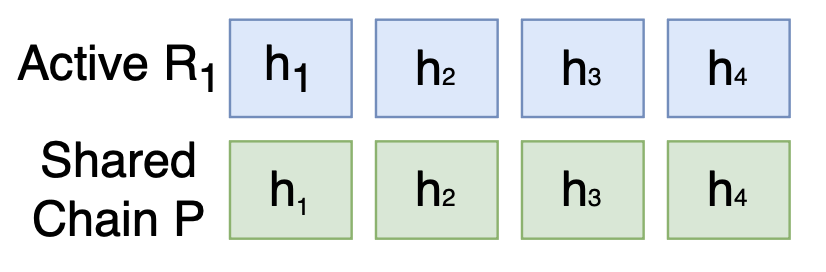
\includegraphics[width=\linewidth]{illustration_images/shared_prefix_chain_step1.png}
    \caption{}
    \label{fig:shared_prefix_chain_step1}
\end{subfigure}
\hfill
\begin{subfigure}{0.24\textwidth}
    \centering
    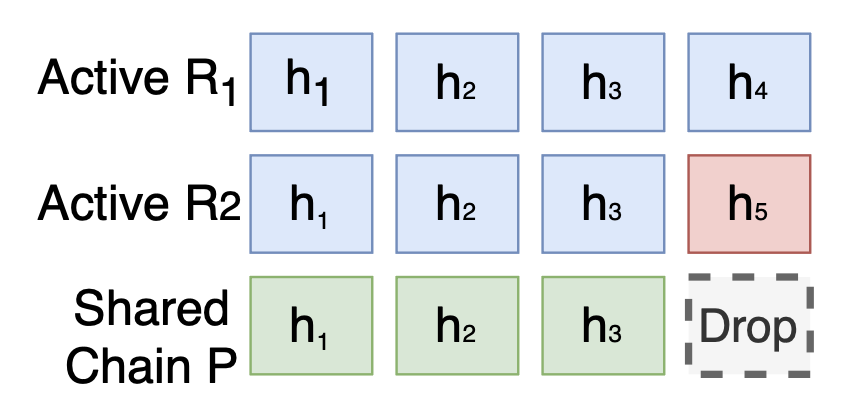
\includegraphics[width=\linewidth]{illustration_images/shared_prefix_chain_step2.png}
    \caption{}
    \label{fig:shared_prefix_chain_step2}
\end{subfigure}
\hfill
\begin{subfigure}{0.24\textwidth}
    \centering
    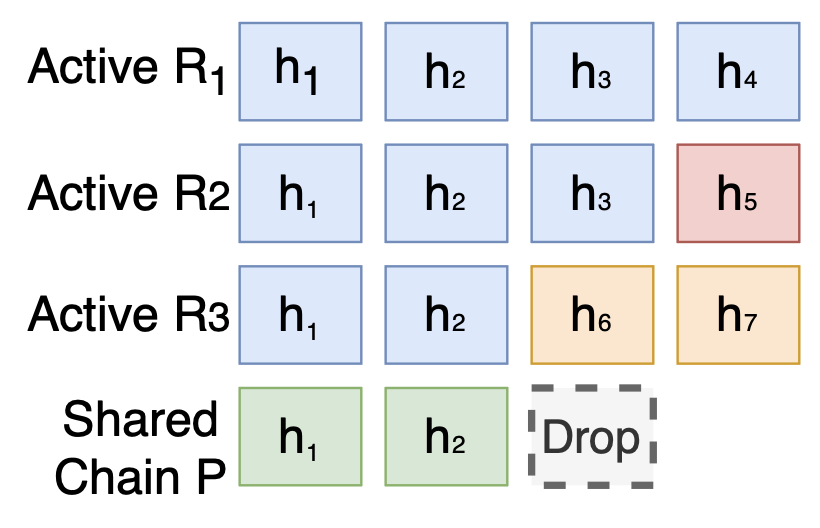
\includegraphics[width=\linewidth]{illustration_images/shared_prefix_chain_step3.png}
    \caption{}
    \label{fig:shared_prefix_chain_step3}
\end{subfigure}
\hfill
\begin{subfigure}{0.24\textwidth}
    \centering
    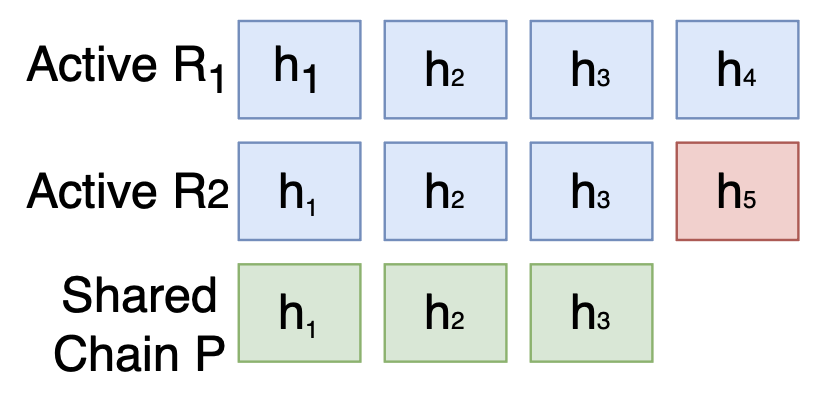
\includegraphics[width=\linewidth]{illustration_images/shared_prefix_chain_step4.png}
    \caption{}
    \label{fig:shared_prefix_chain_step4}
\end{subfigure}

\caption{An example of shared prefix chain workflow. We initially have just a single active request $R_1$ with four prefix hash chunks, so the shared prefix chain is also the same as its hash vector, as shown in figure~\ref{fig:shared_prefix_chain_step1}. We then activate $R_2$, which does not have the last level common with $R_1$, and thus the chain size reduces by one~\ref{fig:shared_prefix_chain_step2}. Similarly, as shown in~\ref{fig:shared_prefix_chain_step3}, activation of another request $R_3$ leads to further reduction in the chain size. Now, $R_3$ finishes its execution first, so we remove it from the set of active requests, and therefore this gives an opportunity to extend the chain~\ref{fig:shared_prefix_chain_step4}.}
\label{fig:shared_prefix_chain_workflow}
\end{figure*}


\subsubsection*{Optimizations}
\paragraph{Result caching.}
$\textsc{FindBest}()$ may be called repeatedly within a single scheduling round without any intervening state change.  We cache its last result—a four-tuple\\ $(r^*, \mathit{chunks\_before}, \mathit{chunks\_after}, \mathit{peers})$ and return it immediately on subsequent calls until a mutation invalidates the flag. 

\paragraph{Lazy heap updates.}
The waiting heap uses \emph{lazy deletion}: when a request's missing count changes, we push a new $(m_r, r)$ entry rather than updating the existing one in place. Stale entries (where the recorded $m$ differs from $\mathit{miss}[r]$) are silently skipped during $\textsc{FindBest}$. This avoids the $O(W)$ cost of a linear heap search and keeps activation and completion at $O(C \cdot W_h \cdot \log W)$ total, where $W_h$ is the average number of waiting requests per hash.

\paragraph{Incremental shared prefix chain maintenance.}
Recomputing the shared prefix chain from scratch after every activate or finish event would cost $O(A \cdot C)$, where $A$ is the active-set size. Instead, we exploit the fact that activation can only \emph{shrink} the chain and completion can only \emph{grow} it. On activation, we truncate $P$ at the first mismatch with the new request's hash vector in $O(L)$; on completion, we attempt a forward extension beyond the current chain length, stopping at the first disagreement, again in $O(L + C_{\max})$.

Additionally, all major hash tables and vectors pre-allocate capacity at construction time, eliminating rehash latency and reallocation during high-throughput operation.

\subsubsection*{Complexity Analysis}
Table~\ref{tab:complexity} summarizes the time complexity of each operation. $T$ is the average number of tokens per request, $C$ is the average number of chunks per request, $W$ is the number of waiting requests, and $W_h$ is the average number of waiting requests sharing a given hash (typically $W_h \ll W$).

\begin{table}[H]
\centering
\caption{Time complexity of CHT scheduler operations.}
\label{tab:complexity}
\begin{tabular}{ll}
\hline
\textbf{Operation} & \textbf{Complexity}\\
\hline
Insert request            & $O(T + C \log W)$ \\
Activate request          & $O(C \cdot W_h \cdot \log W)$ \\
Update chain on activate  & $O(L)$ \\
Finish request            & $O(C \cdot W_h \cdot \log W)$ \\
Update chain on finish    & $O(L + C_{\max})$ \\
Find best request         & $O(\log W)$ (cached: $O(1)$) \\
Remove request            & $O(C)$ \\
\hline
\end{tabular}
\end{table}

Here $L \le C$ is the current shared chain length, and $C_{\max}$ is the maximum number of chunks in any active request. Because result caching eliminates redundant heap traversals between working-set changes, the dominant cost in practice is the $O(C \cdot W_k \cdot \log W)$ propagation step in activate and finish, which updates the missing counts of all affected waiting requests.

\subsection{Batching and Reinforcement Learning}
\textcolor{red}{any visualizations for these RL policies needed?}

So far, the CHT provides us with an efficient way to find the best next request to add to the batch, the one that maximizes prefix reuse. But it does not tell us \emph{when to stop}. Adding more requests always increases GPU utilization, but at some point, the shared prefix starts to shrink, hurting locality. This section describes how we frame this stop/continue decision as a learning problem and present three policies of increasing complexity: a hand-crafted heuristic that encodes domain intuition, a contextual bandit that learns from experience without temporal structure, and a Q-learning agent that reasons about long-term throughput.

As highlighted in \S\ref{sec:system_overview}, the scheduler incrementally builds a decoding batch by repeatedly selecting the lowest-cost waiting request via the CHT and deciding whether to add it to the current batch or dispatch the batch as-is. This stop/continue decision is the crux of the batching problem. 

\subsubsection*{State, Actions, and Reward}
At each step of batch formation, the scheduler observes a state
\[
s = (\mathit{batch\_size},\; \mathit{chunks\_before},\; \mathit{chunks\_after},\;\mathit{requests\_waiting})
\]
and takes a binary action $a \in \{\textsc{Add}, \textsc{Stop}\}$. Here, $\mathit{batch\_size}$ denotes the number of requests that are already in the batch, which is a proxy for current GPU utilization. $\mathit{chunks\_before}$ is the shared-prefix chain length \emph{before} adding the candidate request; $\mathit{chunks\_after}$ is the chain length after hypothetically adding it (obtained from $\textsc{FindBest}$); and $\mathit{requests\_waiting}$ is the number of waiting requests that share the prefix up to level $\mathit{chunks\_after}$, indicating whether the locality cost of this addition will be compensated by future activations. Together, these four values capture both the current GPU utilization (batch size) and the cost of the proposed addition to prefix locality, summarized by the chunk loss $\Delta = \mathit{chunks\_before} - \mathit{chunks\_after}$).

Both learning policies share the same reward signal: the decode throughput of the dispatched batch,

\[
\mathcal{R} = \text{throughput}_{\mathrm{decode}}
\]

Maximizing this reward simultaneously encourages large batches (better GPU utilization) and short decode times (better prefix locality). Both policies also operate over the same discretized state space: $\mathit{batch\_size}$ and $\mathit{requests\_waiting}$ are mapped to exponential bins, while the chunk loss $\Delta$ is mapped to a coarser set of thresholds. The discretized state is a triple $(\hat{b}, \hat{\Delta}, \hat{w})$, where each hat denotes the bin index. The resulting table is small enough to store in a hash map and converges quickly, even under moderate traffic.

\subsubsection*{Heuristic Policy}
Before introducing any learning, we establish a baseline that encodes domain intuition directly as rules. The heuristic is designed around two competing goals: \emph{maximizing GPU utilization} by filling the batch as much as possible and \emph{preserving prefix locality} by avoiding candidates that cause large drops in the shared prefix chain. The heuristic always adds a candidate that does not hurt the shared chain at all—a free addition. When the batch is still very small and GPU utilization is clearly low, it tolerates a slightly larger locality cost to avoid dispatching an underutilized batch. In the general case, it accepts a candidate only if the chunk loss is within a small tolerance. Finally, when many waiting requests share the same prefix level, it allows a marginally higher locality cost since the short-term penalty is likely to be offset by the homogeneous additions that follow. If none of these conditions are met, the heuristic stops and dispatches the current batch.

This policy requires no training and converges immediately, but its thresholds are fixed and cannot adapt to shifts in workload distribution.

\subsubsection*{Contextual Bandit}
To move beyond hand-tuned thresholds, we implement a contextual bandit using Upper Confidence Bound (UCB) selection~\cite{auer2002finite}. The bandit treats each batch-construction call as an independent decision: given the discretized state $\hat{s} = (\hat{b}, \hat{\Delta}, \hat{w})$, it selects the action that maximizes
\[
  \mathrm{UCB}(\hat{s},a) = \frac{\mu(\hat{s},a)}{n(\hat{s},a)} + c\sqrt{\frac{\ln N}{n(\hat{s},a)}}
\]
where $\mu(\hat{s}, a)$ is the cumulative reward for taking action $a$ in state $\hat{s}$, $n(\hat{s}, a)$ is the number of times that pair has been selected, $N$ is the total number of steps, and $c$ is the exploration coefficient. The first term favors actions that have historically yielded high throughput; the second term ensures that under-explored actions are tried sufficiently often.

Because the bandit discards temporal structure entirely, it does not reason about how today's batching decision affects the state of the queue for the next batch, it can miss opportunities where a short-term locality sacrifice leads to a better-amortized sequence of future batches. This motivates the full reinforcement learning approach.

\subsubsection*{Q-Learning Policy}
To capture the temporal dependencies that the bandit ignores, we model batch construction as an episodic reinforcement learning problem. A new episode begins each time the scheduler starts forming a fresh batch and terminates when it issues \textsc{Stop} or the waiting queue is exhausted. The Q-table~\cite{watkins1992} stores a value $Q(s, a)$ for every (discretized state, action) pair and is updated upon each batch completion via the standard Bellman update:

\[
Q(s, a) \; \leftarrow\; Q(s, a) + \alpha\bigl[r + \gamma \max_{a'} Q(s', a') - Q(s, a)\bigr]
\]

where $r$ is the observed throughput reward, $s'$ is the state at the start of the \emph{next} batch formation, $\alpha$ is the learning rate, and $\gamma$ is the discount factor. The discount factor encodes that the agent values near-term throughput slightly more than long-term gains, which matches the real-time nature of an inference server. During training, $\varepsilon$ starts at $1.0$ (fully random) and decays linearly to $\varepsilon_{\min}$ over a configurable number of steps, after which the policy is nearly deterministic.

\subsubsection*{The \textsc{BuildBatch} Procedure}
Algorithm~\ref{alg:rl_batch} shows how all three policies fit into the same batch-construction loop. At each iteration, \textsc{FindBest} (Algorithm~\ref{alg:find_best}) is called to retrieve the lowest-cost candidate from the CHT along with its chain statistics $c_{\mathrm{before}}$, $c_{\mathrm{after}}$, and the number of waiting requests $w$ that share the same prefix level. These four values are assembled into the state $s$ and passed to whichever policy $\pi$ is active—heuristic, bandit, or Q-learning agent—which returns either \textsc{Add} or \textsc{Stop}. If \textsc{Add}, the candidate is activated and appended to the batch; if \textsc{Stop}, the loop exits and the batch is dispatched immediately. Once the batch executes, the observed decode throughput serves as the reward signal: the bandit updates its count-and-mean tables, while the Q-learning agent applies the Bellman update above. The heuristic requires no update. 

\begin{algorithm}[H]
\caption{$\textsc{BuildBatch}()$}
\label{alg:rl_batch}
\begin{algorithmic}[1]
\Require Waiting queue $Q$; policy $\pi$ (heuristic, bandit, or Q-learning); discount $\gamma$; learning rate $\alpha$
\Ensure Batch $B$ ready for one decode iteration
\State $B \gets \emptyset$
\While{$Q \neq \emptyset$}
    \State $(r^*, c_{\mathrm{before}}, c_{\mathrm{after}}, w) \gets \textsc{FindBest}()$
    \If{$r^* = \bot$} \textbf{break} \EndIf
    \State $s \gets (|B|,\; c_{\mathrm{before}},\; c_{\mathrm{after}},\; w)$
    \State $a \gets \pi(s)$ \Comment{heuristic rule / UCB look-up / $\varepsilon$-greedy Q-table}
    \If{$a = \textsc{Stop}$} \textbf{break} \EndIf
    \State $\textsc{Activate}(r^*)$;\quad $B \gets B \cup \{r^*\}$
\EndWhile
\State $\text{throughput}_{\mathrm{decode}} \gets \textsc{ExecuteBatch}(B)$
\State \textbf{Update} $\pi$ with observed reward $\text{throughput}_{\mathrm{decode}}$ \Comment{no-op for heuristic}
\State \Return $B$
\end{algorithmic}
\end{algorithm}






\subsection{Integration with vLLM and SGLang}
We integrate our scheduler as a lightweight layer on top of both vLLM's~\cite{kwon2023efficient} and SGLang's~\cite{zheng2024sglangefficientexecutionstructured} existing request management pipeline. The Chunked Hash Tree (implemented in C++), shared prefix chain tracking, and reinforcement learning policies operate entirely at the scheduler level.

\section{Evaluation}
\label{sec:eval}
In this section, we evaluate the performance of our scheduler under a variety of workloads.

\subsection{Experimental Setup}

\textbf{Model and server configurations.} We use Qwen \cite{qwen} models with 2B, 8B, and 13B parameters, LLama3 \cite{llama3modelcard} with 7B and 8B parameters, and LongChat \cite{longchat2023} with 13B parameters. For all of our experiments, we use the RTX6000 Ada Generation GPU \cite{nvidia_rtx6000_datasheet} with an HBM of 48GB and an L2 cache size of 96MB.

\textbf{Workloads:} Similar to prior work, the arrival pattern of requests is generated by a Poisson process. The input lengths and output lengths of requests are sampled from the following real-world datasets.

L-Eval \cite{an2023leval}: It contains human-labeled query-response pairs on diverse tasks, such as summarization and question answering. The range of sequence length in this dataset is 2.7K - 210.5K tokens.

LongBench \cite{bai2024longbench2} encompasses a curated subsample of elongated data, ranging from 4K to 10K context length, excerpts from 21 datasets across 6 categories, including tasks like multi-document question answering, summarization, and code completion.


\textbf{Baseline 1: vLLM \cite{kwon2023efficient}} vLLM is a high-throughput LLM serving system designed to improve GPU memory efficiency during autoregressive decoding. Its core contribution is PagedAttention, an attention mechanism that stores the key–value (KV) cache in fixed-size blocks rather than contiguous memory. Inspired by virtual memory paging in operating systems, PagedAttention allows KV blocks to be allocated on demand and mapped non-contiguously in GPU memory, substantially reducing internal and external fragmentation caused by variable-length prompts and outputs. In addition, vLLM supports KV cache sharing across sequences. We use vLLM version 0.14.0 across all our experiments.

\textbf{Baseline 2: SGLANG \cite{zheng2024sglangefficientexecutionstructured}}
\textcolor{red}{too long, but description necessary as we can't cite anything, SGLANG's paper does not mention about the newer scheduler policies, and we need to show it as a bad design for our chunked hash tree idea to come out}
 SGLANG is a system for efficient execution of structured language model programs, consisting of a Python-embedded frontend language and a co-designed runtime. On the runtime side, SGLANG introduces RadixAttention, which enables automatic KV cache reuse across multiple generation calls by organizing cached prefixes in a radix tree with cache-aware scheduling. This allows SGLANG to exploit multi-level prefix sharing beyond simple system-prompt reuse. We use SGLANG version 0.5.7 across all our experiments.

SGLANG supports multiple request scheduling policies that trade off fairness, throughput, and KV-cache efficiency. These policies fall into two categories: cache-aware and cache-agnostic.
\begin{itemize}
    \item \textbf{Cache-aware policies.} These policies explicitly leverage the radix-tree prefix cache to increase KV reuse:
    \begin{itemize}
        \item \textbf{Longest Prefix Match (LPM):} Prioritizes requests whose input prefixes match the longest cached prefixes. This maximizes immediate KV cache reuse and reduces redundant prefill computation.
        \item \textbf{DFS-Weight:} Traverses the radix cache tree in a depth-first manner and prioritizes branches with more active requests. This groups requests that share deeper prefixes, improving cache locality over time.
    \end{itemize}
    \item \textbf{Cache-agnostic policies.} These policies do not consider prefix sharing and serve as simpler baselines:
    \begin{itemize}
        \item \textbf{First-Come-First-Serve (FCFS):} Schedules requests in arrival order. This is also the fallback policy when prefix caching is disabled.
        \item \textbf{Longest Output First (LOF):} Prioritizes requests with larger maximum generation lengths, which can improve GPU utilization under heavy load.
        \item \textbf{Random:} Randomly shuffles pending requests and is mainly used as a control or stress-test policy.
    \end{itemize}
    \item \textbf{Additional scheduling mechanisms.} In addition to request ordering, SGLANG includes:
    \begin{itemize}
        \item \textbf{In-batch prefix caching:} Detects shared prefixes among waiting requests and temporarily deprioritizes redundant ones so that a single request can populate the cache for others.
        \item \textbf{Priority-aware scheduling:} Allows requests to be assigned priorities, which can be combined with FCFS or LOF ordering.
        \item \textbf{Priority-based preemption:} Enables higher-priority requests to preempt running lower-priority ones when token or memory budgets are limited.
    \end{itemize}
\end{itemize}

\textbf{Baseline 3: Dynamic Batching \cite{pang2025optimizing}.} 
\textcolor{red}{not necessary as a baseline, not relevant?} Dynamic batching treats the batch size as a runtime decision variable rather than a fixed hyper-parameter. It continuously adjusts the active batch size based on real-time GPU memory utilization and, optionally, decoding latency constraints. The approach employs a memory-aware batch scheduler to prevent KV-cache overcommitment and a latency feedback mechanism to satisfy service-level agreements (SLAs). We implement dynamic batching onin top of vLLM as another scheduler.


\textcolor{red}{
can add more baselines?
\begin{itemize}
    \item fasttree: code not available, for end-to-end inference
    \item batchllm: does not operate in dynamic workload settings, can compare it with in a batch like setting? again code not available
    \item promptcache: maintains a database of kv cache, not directly related to our stuff?
    \item sarathi serve: can add as a baseline, which is below vllm fcfs, but not relevant otherwise?
    \item pod attention: some kind of parallel optimization, although to use, we will have to implement stuff on sarathi serve
    \item loong serve and other baselines: go through dropbox and recent conference releases again to find more stuff (TODO)
\end{itemize}
}



\textbf{Key Metrics.} Throughput (req/s) measures how many requests the system can complete per second and indicates its overall serving capacity. Higher throughput indicates better utilization of GPU compute and memory resources.

Time Between Tokens (TBT) is the average time gap between consecutive generated tokens during decoding. It reflects how smoothly and responsively the model produces output, which is especially important for interactive settings.

End-to-end latency measures the total time from when a request is submitted until the full response is generated, including both prefill and decoding stages. This metric directly captures the user-perceived response time.

Normalized latency is defined as the end-to-end latency divided by the output sequence length. It helps account for varying response lengths and enables a fair comparison across different workloads.

\textcolor{red}{out tokens/sec needed?}

\begin{figure}[H]
    \centering
    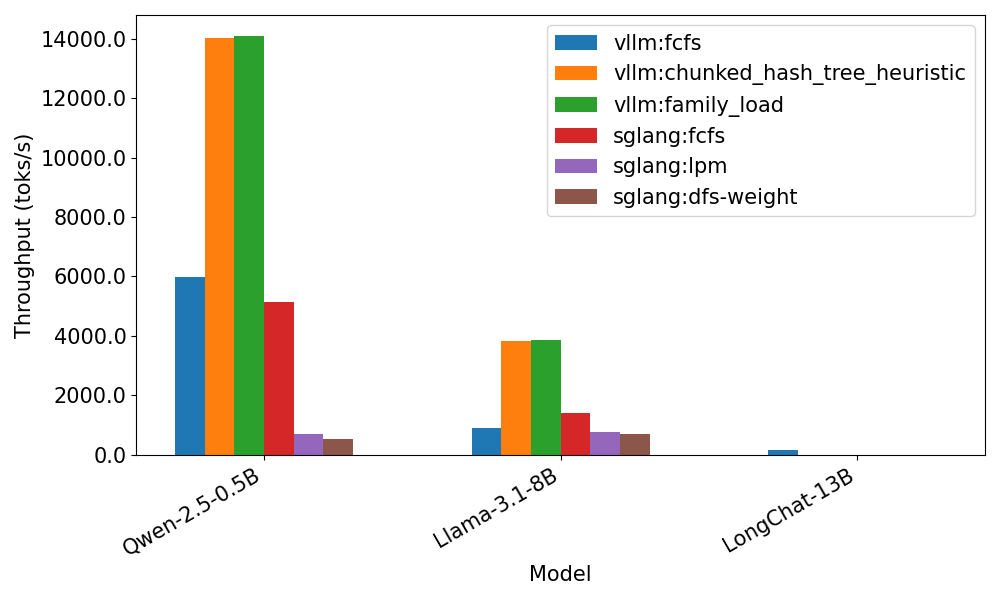
\includegraphics[width=0.8\linewidth]{results/throughput_vs_models_length_5000_families_5.png}
    \caption{Throughput comparison for various models under different scheduling policies with average shared context length of 5000 tokens and 5 prefix groups}
    \label{fig:throughput-models-len5000-fam-5}
\end{figure}

\begin{figure*}[t]
\centering
\begin{subfigure}{0.32\textwidth}
    \centering
    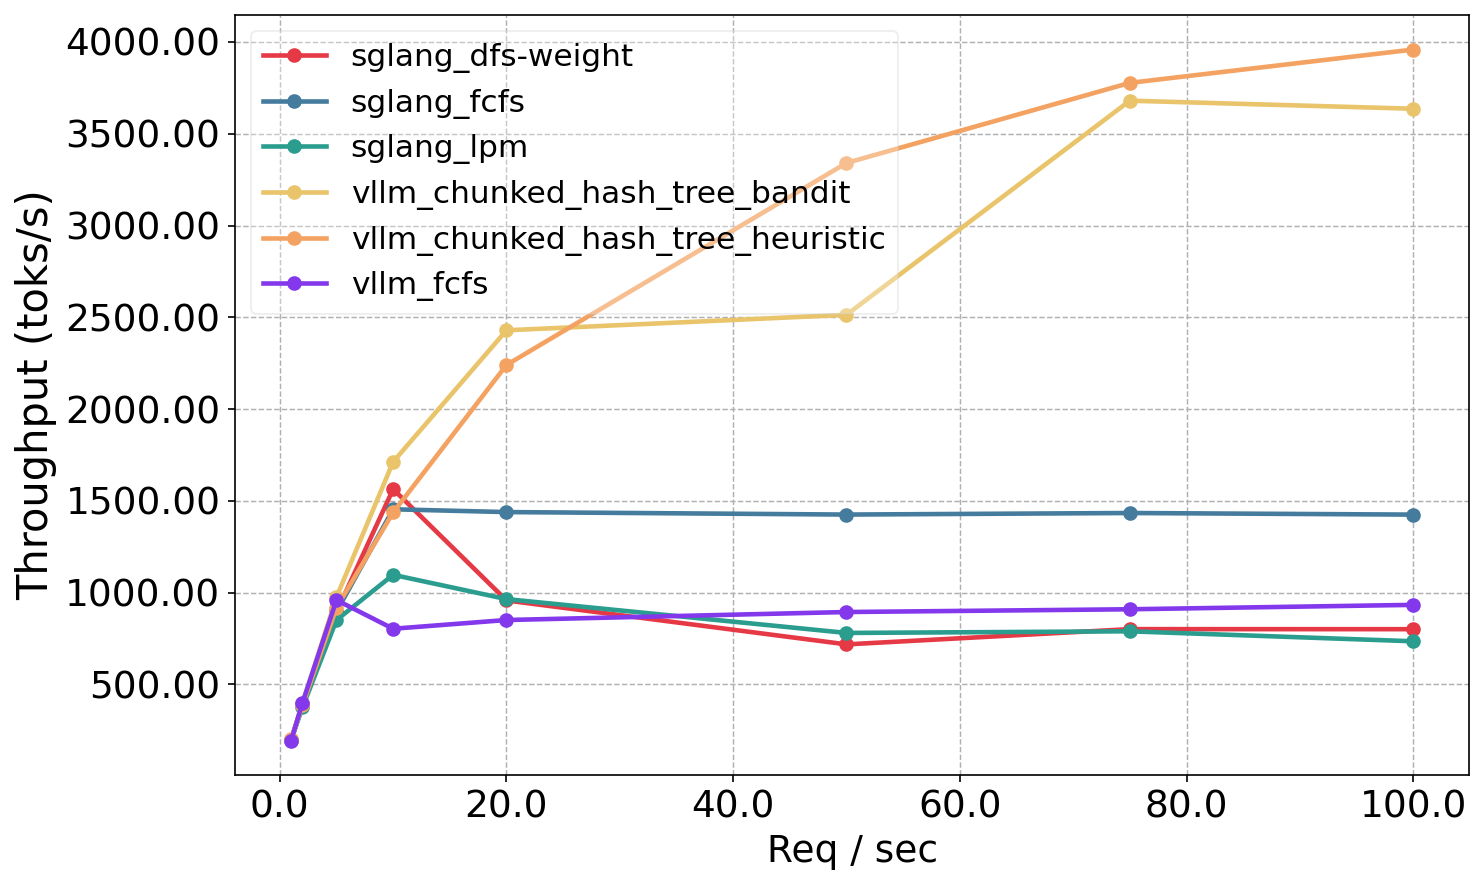
\includegraphics[width=\linewidth]{results/req_per_sec_plots/throughput_vs_rps.png}
    \caption{}
    \label{fig:tp_vs_rps_l_5000_fam_5}
\end{subfigure}
\hfill
\begin{subfigure}{0.32\textwidth}
    \centering
    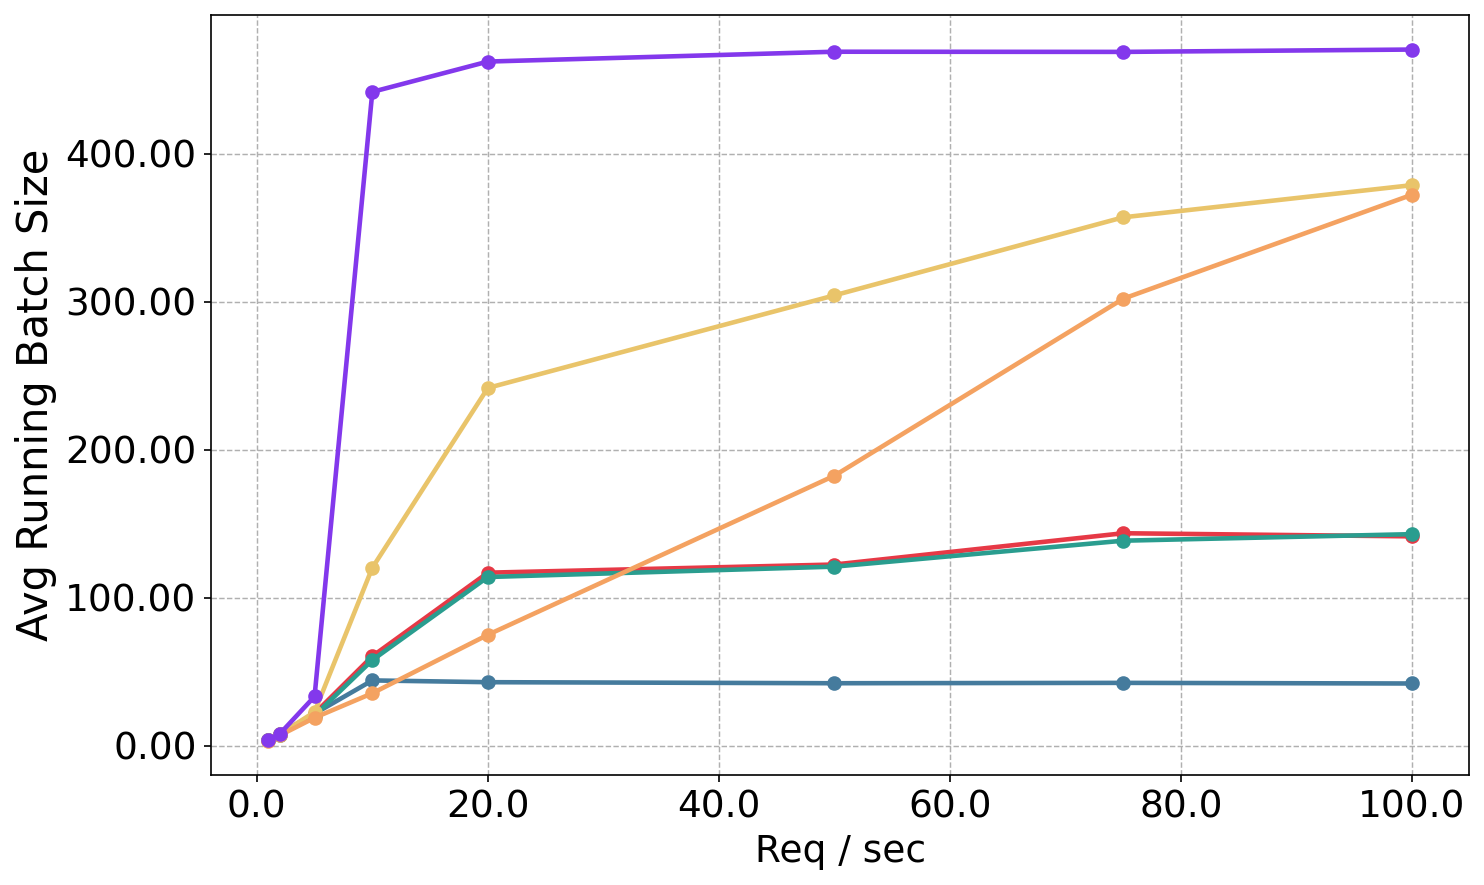
\includegraphics[width=\linewidth]{results/req_per_sec_plots/avg_batch_vs_rps.png}
    \caption{}
    \label{fig:tbt_vs_rps_l_5000_fam_5}
\end{subfigure}
\hfill
\begin{subfigure}{0.32\textwidth}
    \centering
    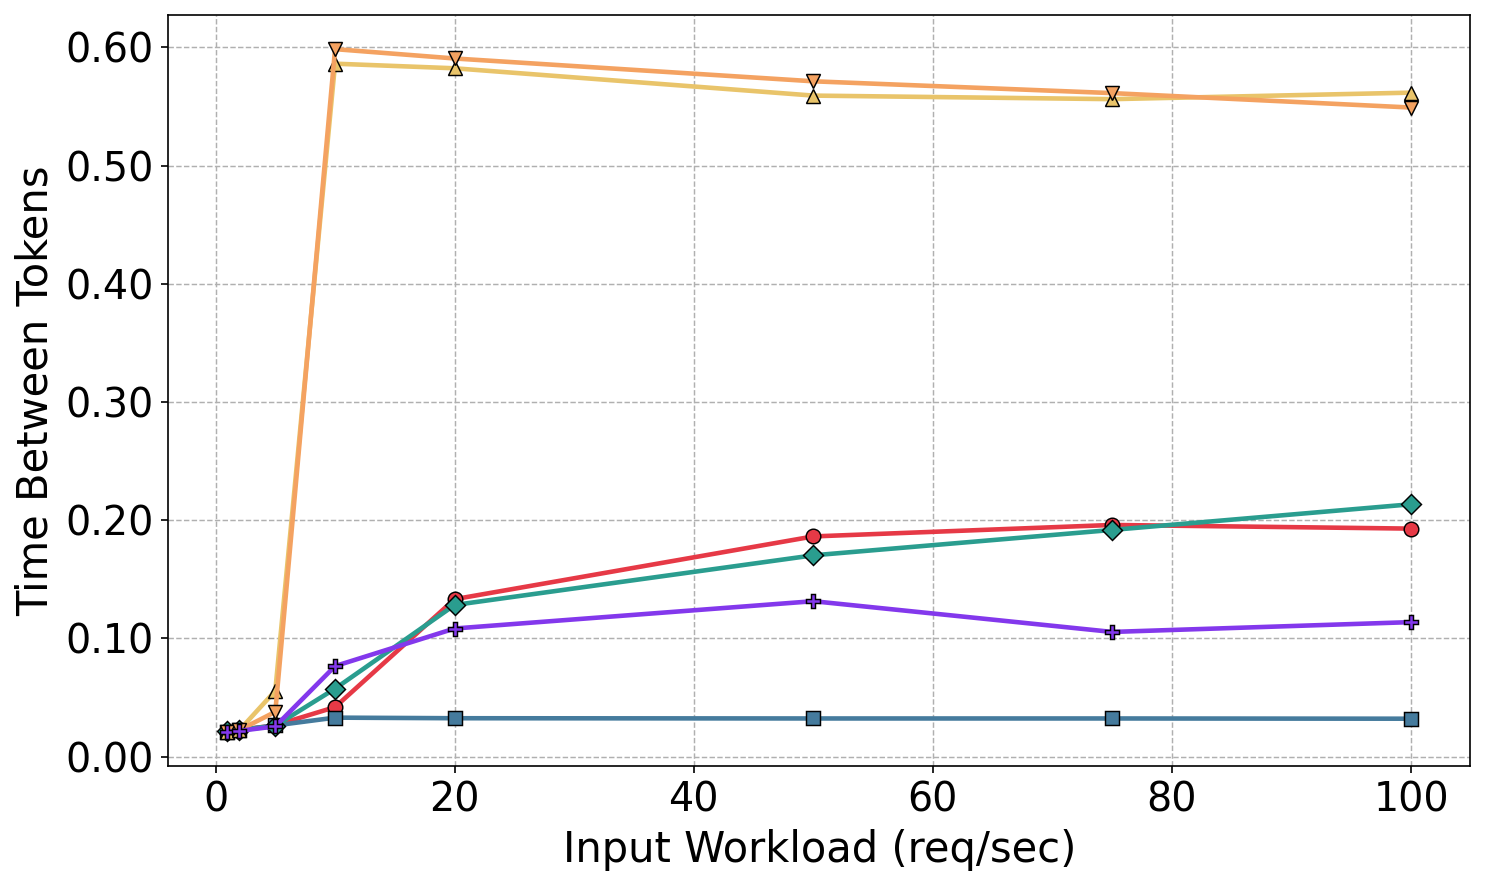
\includegraphics[width=\linewidth]{results/req_per_sec_plots/avg_timediff_vs_rps.png}
    \caption{}
    \label{fig:abs_vs_rps_l_5000_fam_5}
\end{subfigure}

\caption{Various metrics across varying input workload poisson rates. Shared prefix length of 5000 tokens; 5 prefix groups and 200 tokens decode length.}
\label{fig:metrics_vs_rps_l_5000_fam_5}
\end{figure*}

\begin{figure*}[t]
\centering
\begin{subfigure}{0.32\textwidth}
    \centering
    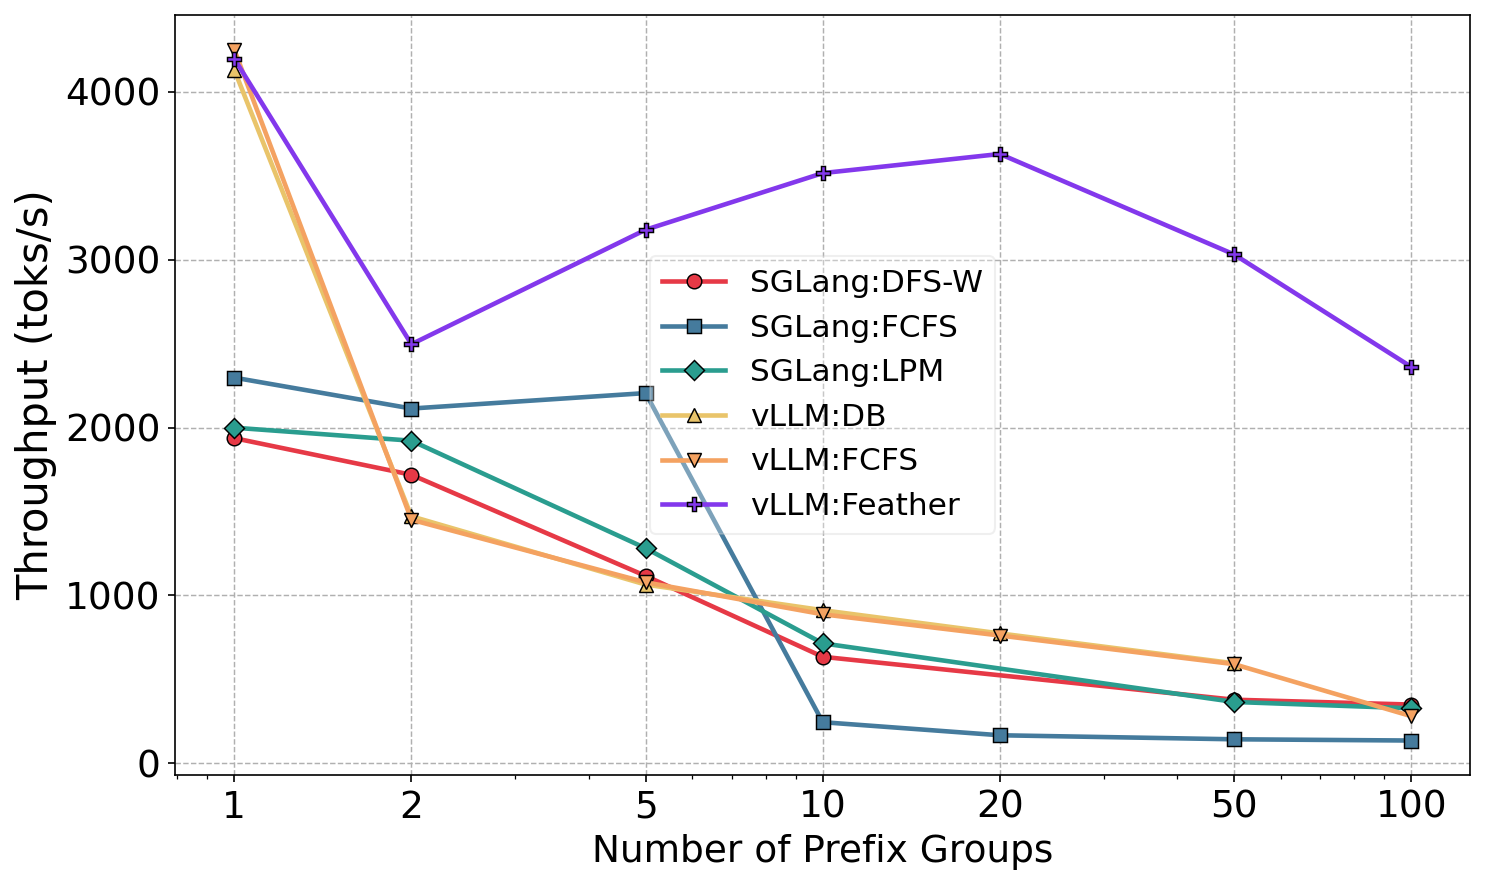
\includegraphics[width=\linewidth]{results/families_plots/throughput_vs_fam.png}
    \caption{}
    \label{fig:tp_vs_fam_l_5000}
\end{subfigure}
\hfill
\begin{subfigure}{0.32\textwidth}
    \centering
    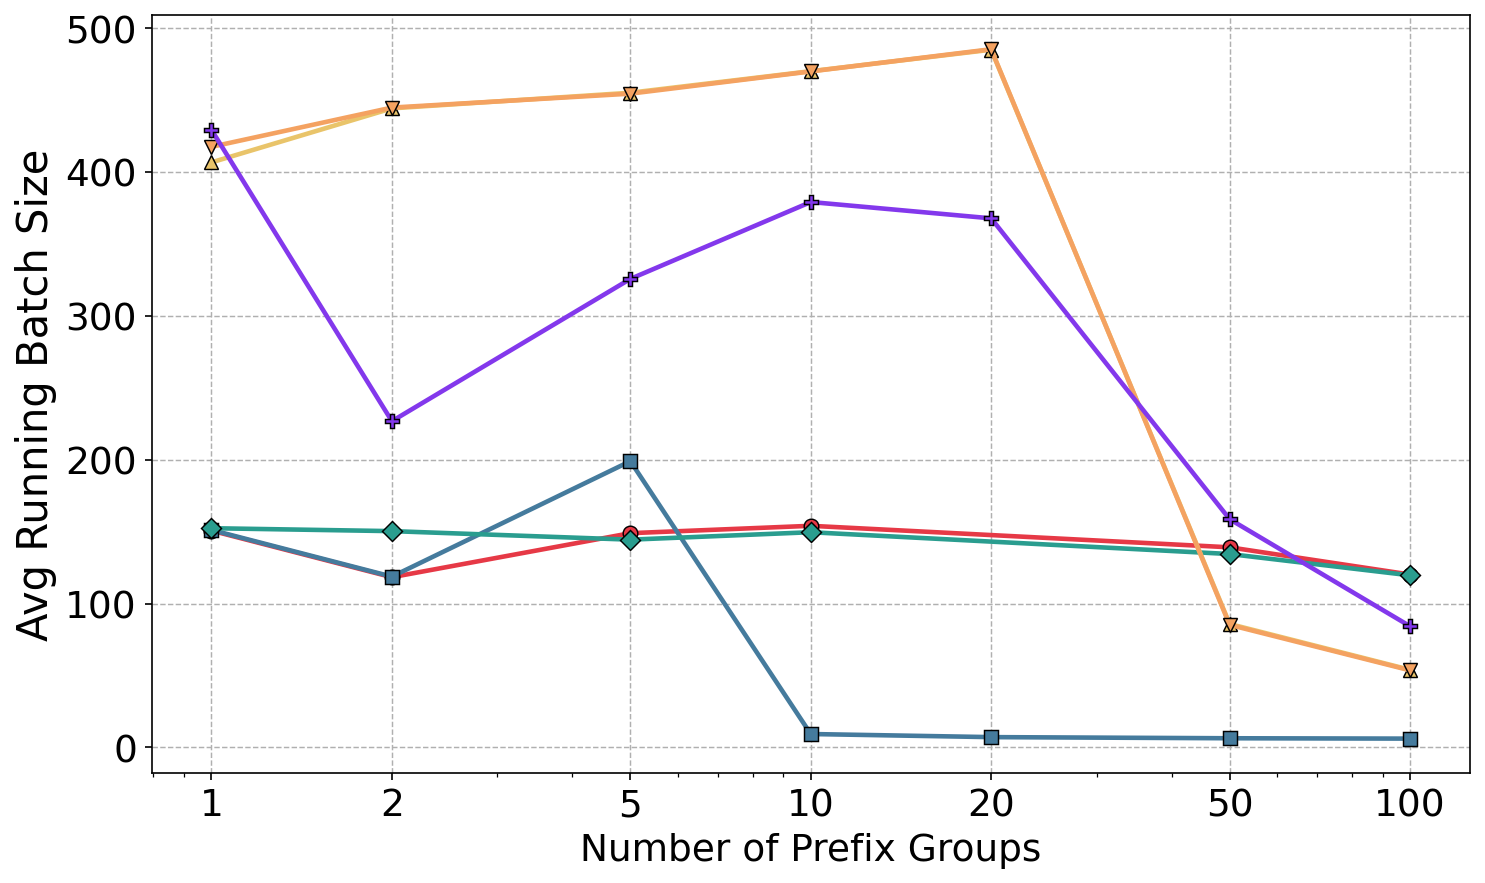
\includegraphics[width=\linewidth]{results/families_plots/avg_batch_vs_fam.png}
    \caption{}
    \label{fig:tbt_vs_fam_l_5000}
\end{subfigure}
\hfill
\begin{subfigure}{0.32\textwidth}
    \centering
    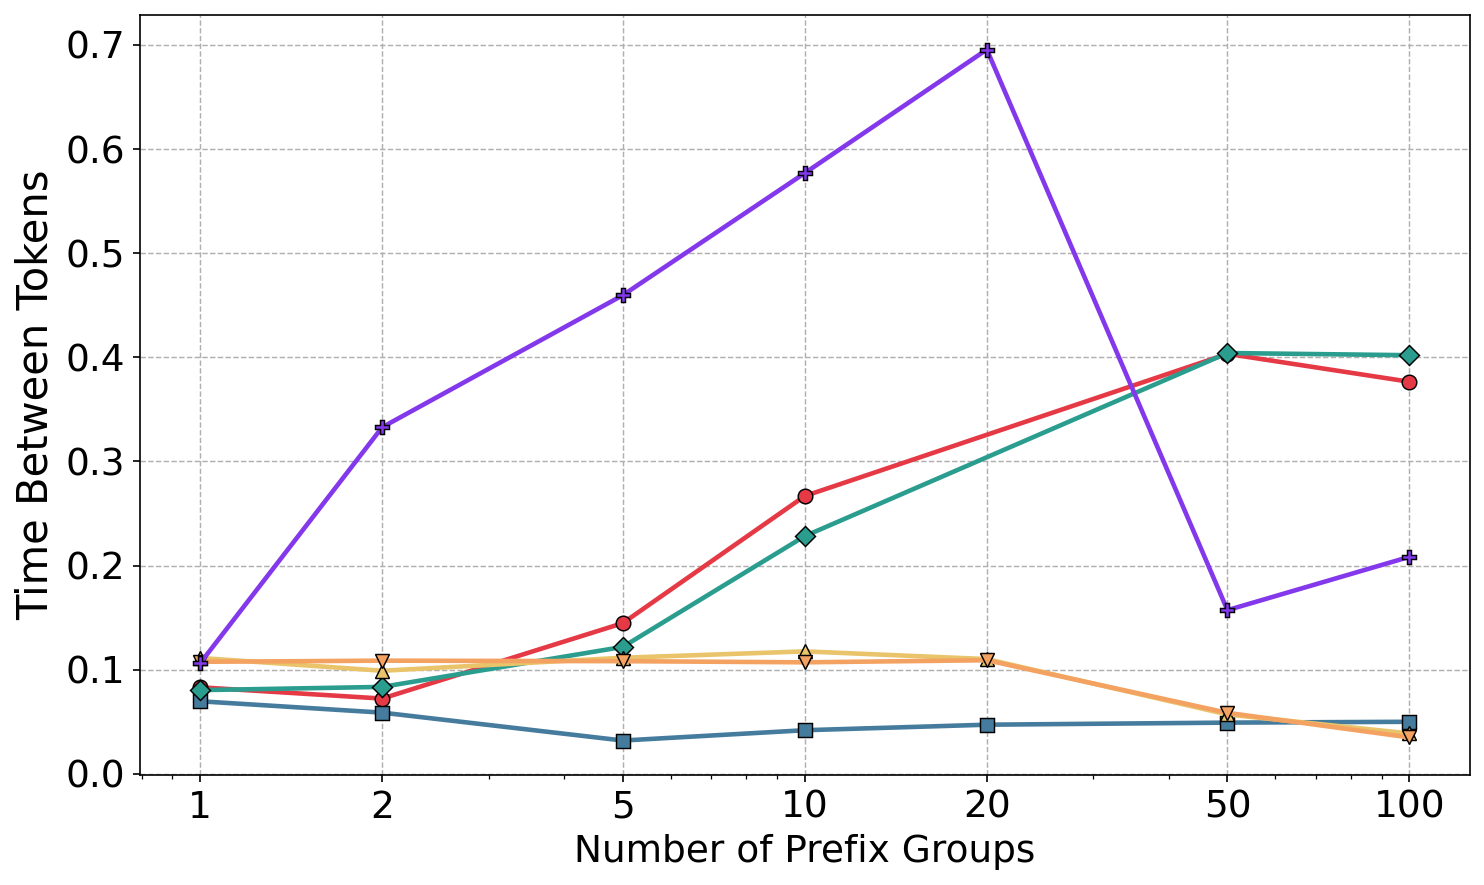
\includegraphics[width=\linewidth]{results/families_plots/avg_timediff_vs_fam.png}
    \caption{}
    \label{fig:abs_vs_fam_l_5000}
\end{subfigure}

\caption{Various metrics across varying number of prefix groups. Shared prefix length of 5000 tokens; 500 input request poisson rate and 200 tokens decode length.}
\label{fig:metrics_vs_fam_l_5000}
\end{figure*}

\begin{figure*}[t]
\centering
\begin{subfigure}{0.32\textwidth}
    \centering
    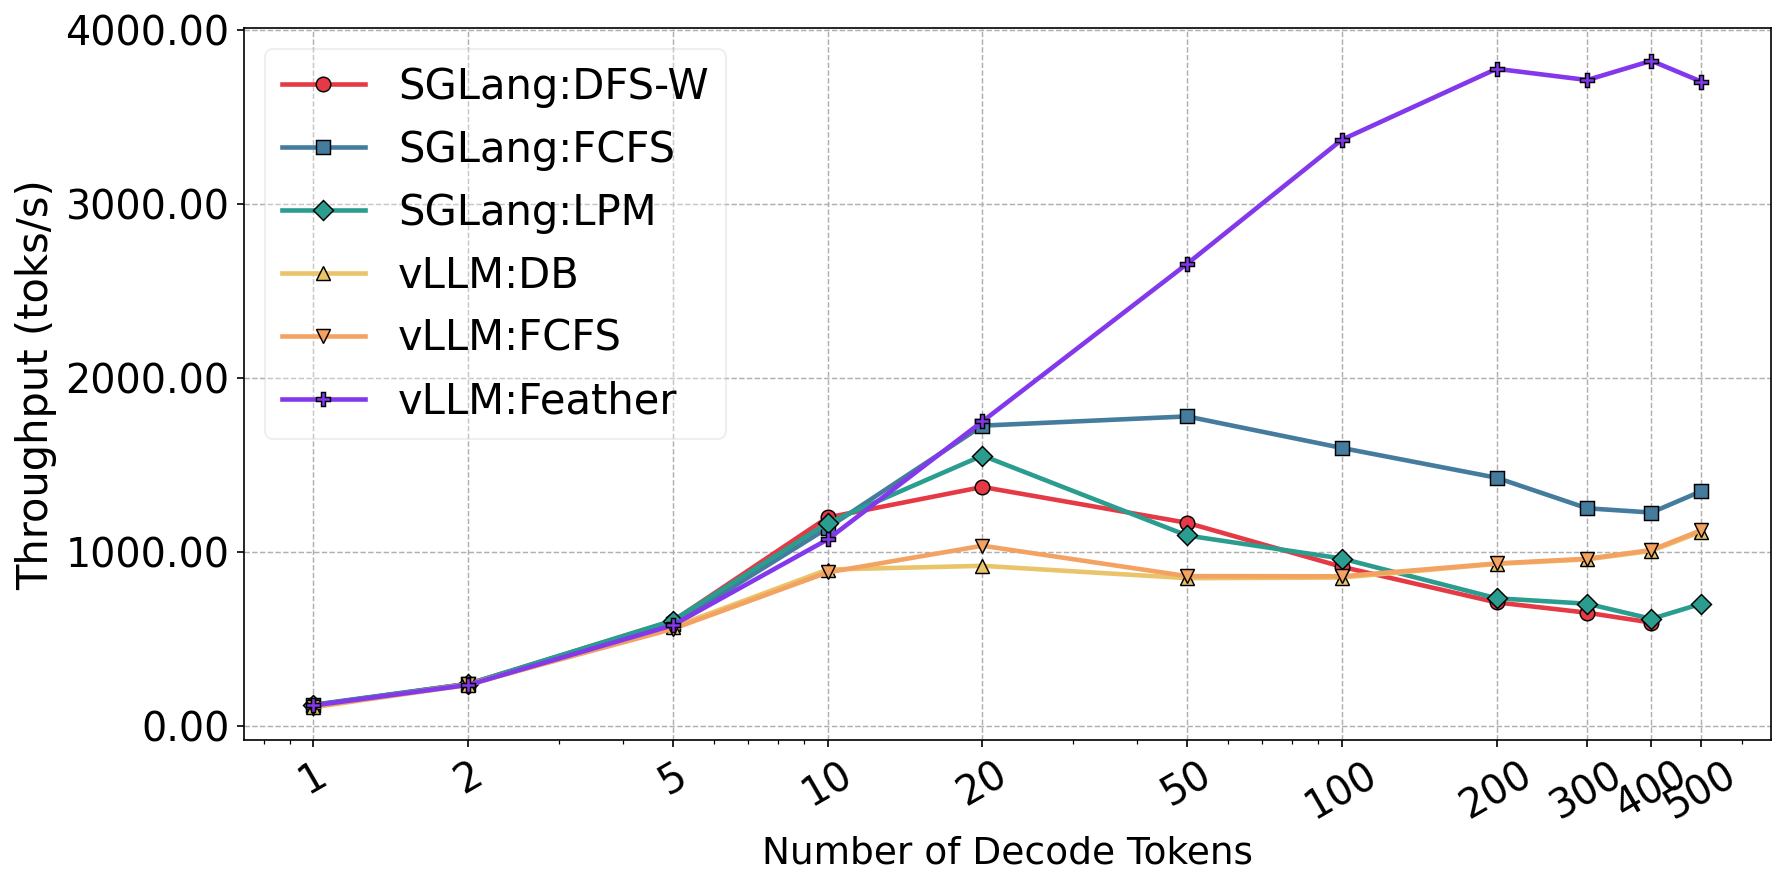
\includegraphics[width=\linewidth]{results/decode_tokens_plots/throughput_vs_tok.png}
    \caption{}
    \label{fig:tp_vs_tok_l_5000}
\end{subfigure}
\hfill
\begin{subfigure}{0.32\textwidth}
    \centering
    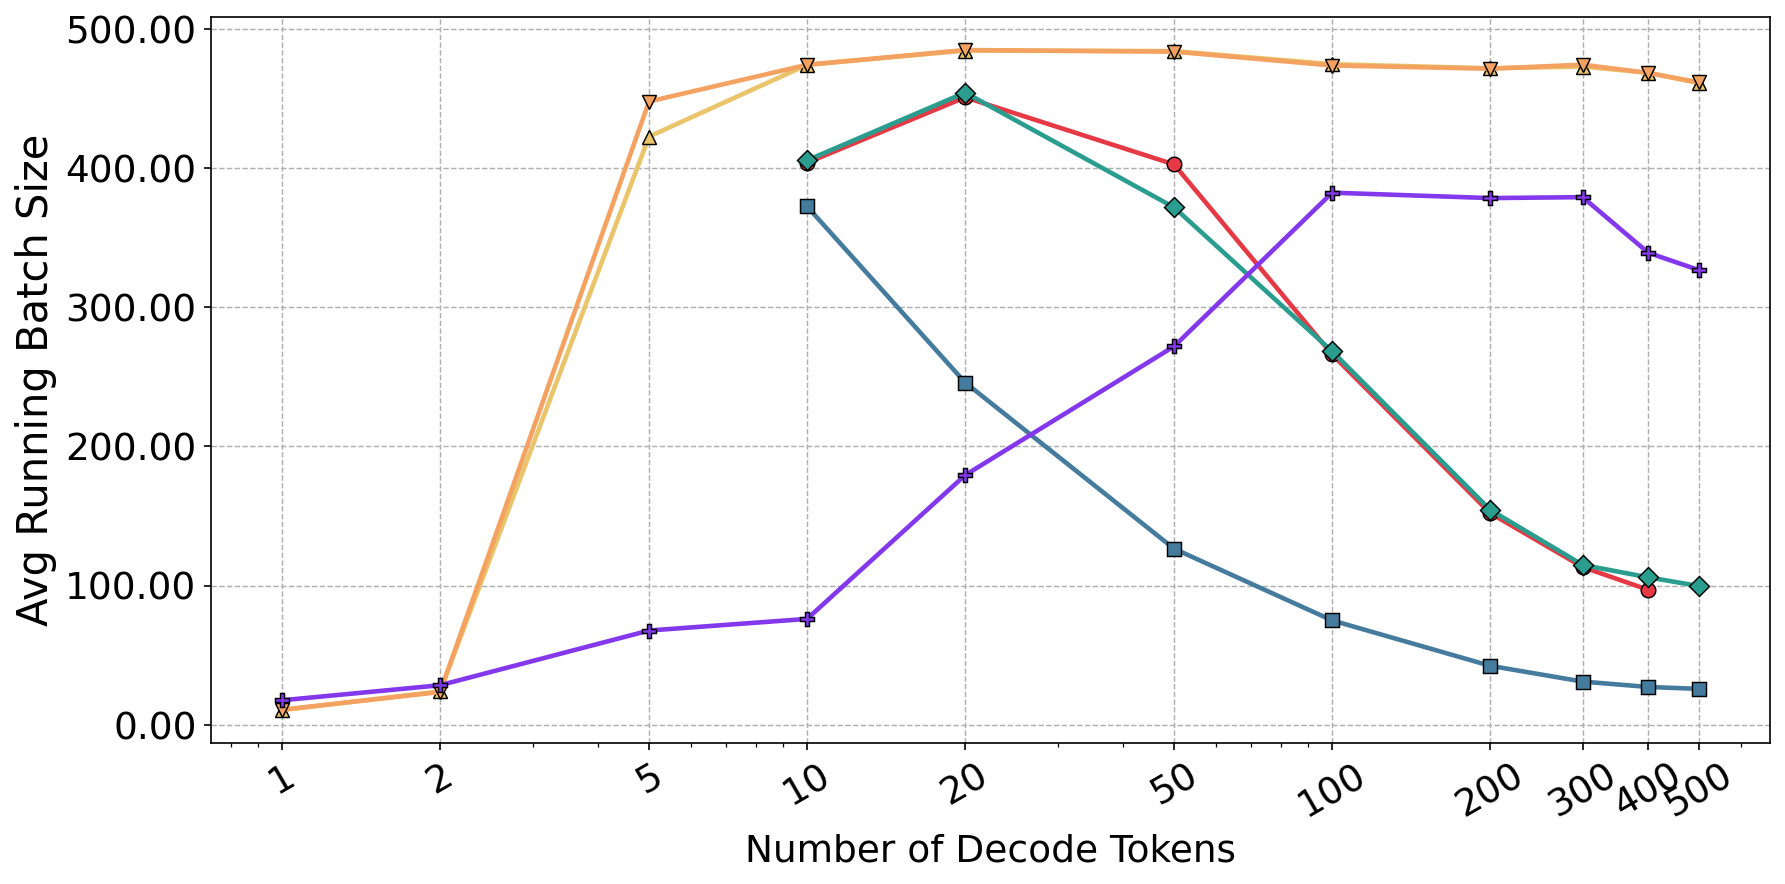
\includegraphics[width=\linewidth]{results/decode_tokens_plots/avg_batch_vs_tok.png}
    \caption{}
    \label{fig:tbt_vs_tok_l_5000}
\end{subfigure}
\hfill
\begin{subfigure}{0.32\textwidth}
    \centering
    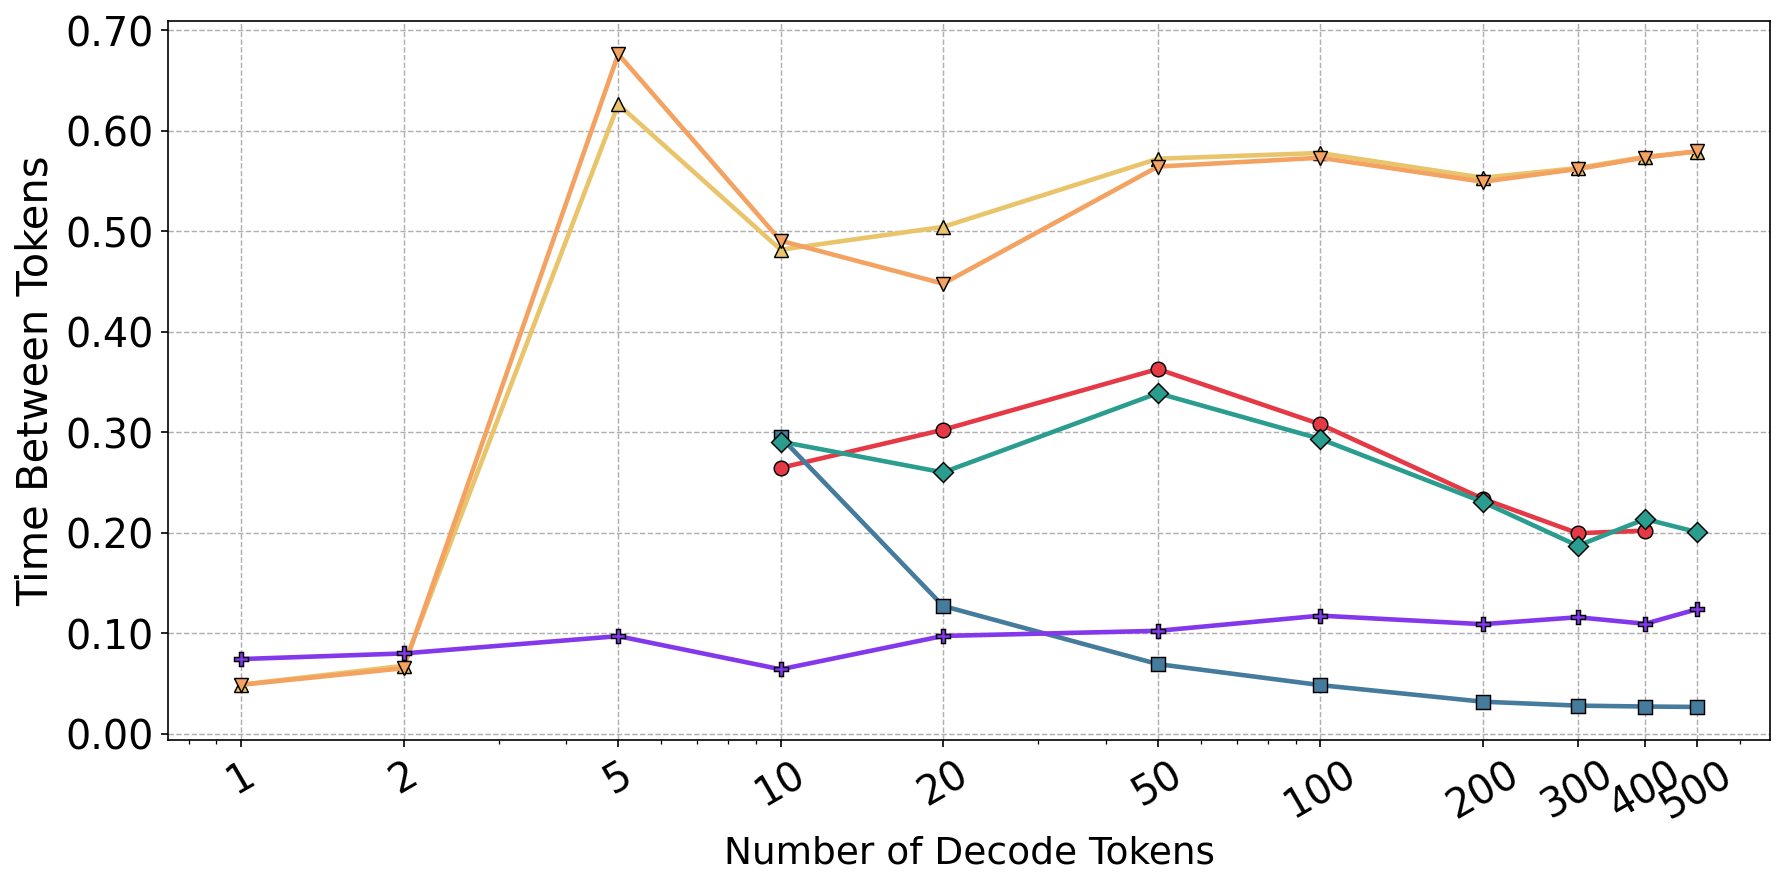
\includegraphics[width=\linewidth]{results/decode_tokens_plots/avg_timediff_vs_tok.png}
    \caption{}
    \label{fig:abs_vs_tok_l_5000}
\end{subfigure}

\caption{Various metrics across varying number of total decode tokens. Shared prefix length of 5000 tokens; 500 input request poisson rate and 5 prefix groups.}
\label{fig:metrics_vs_tok_l_5000}
\end{figure*}

\begin{figure*}[t]
\centering
\begin{subfigure}{0.32\textwidth}
    \centering
    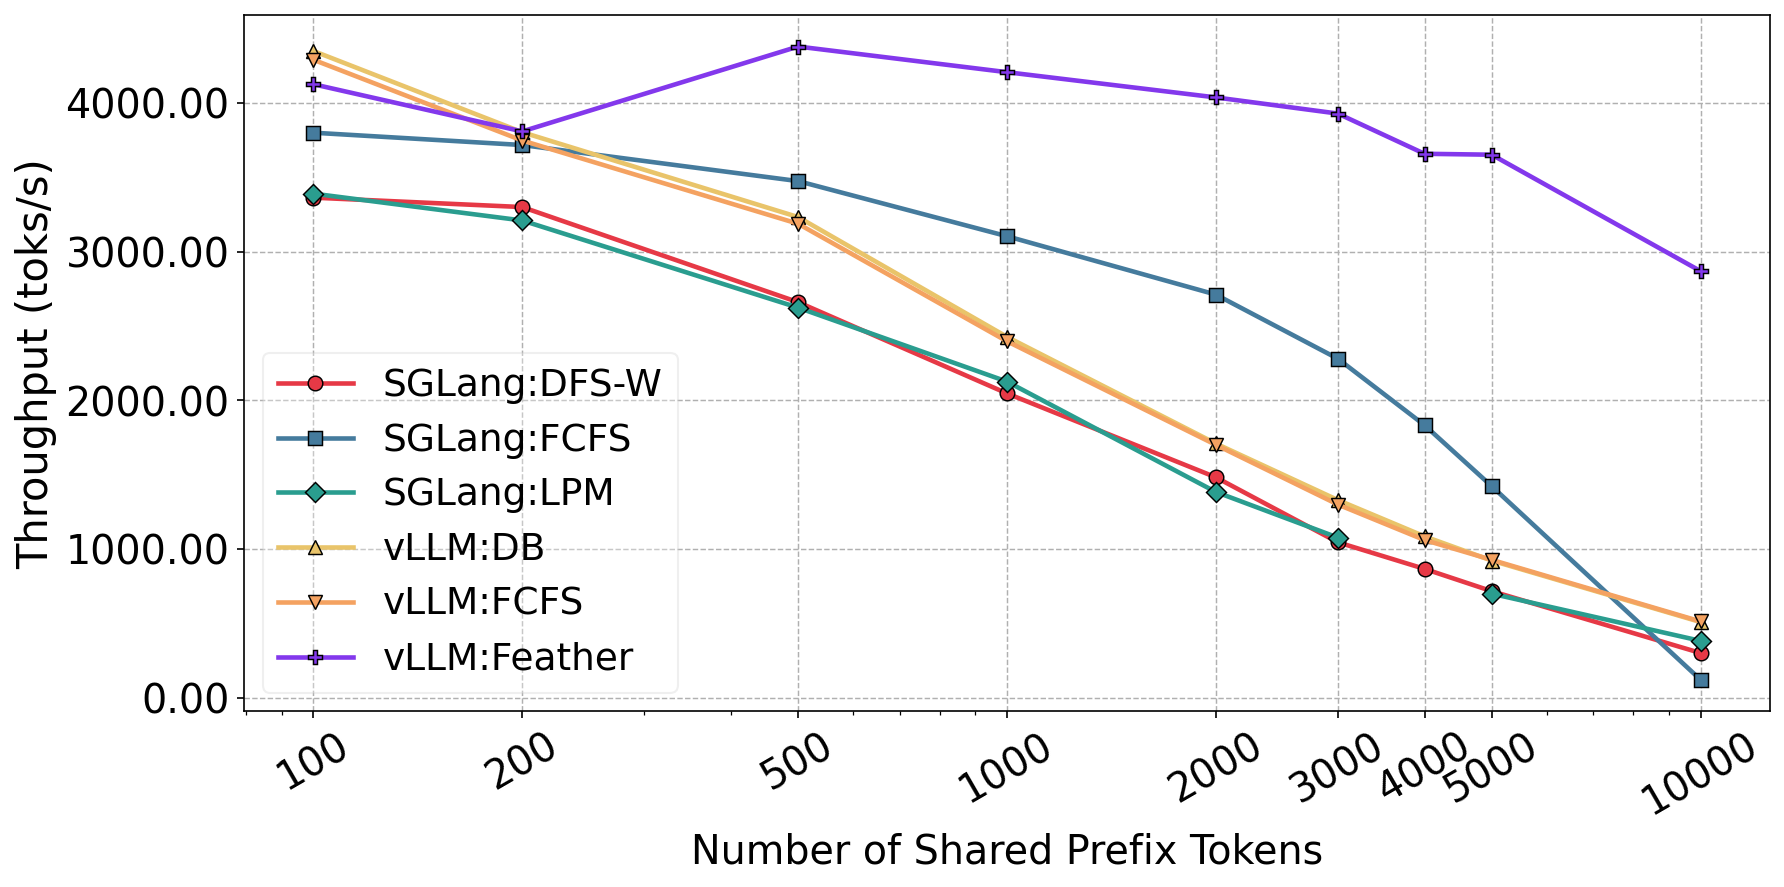
\includegraphics[width=\linewidth]{results/sys_prompt_tokens_plots/throughput_vs_sys_prompt_tokens.png}
    \caption{}
    \label{fig:tp_vs_sys}
\end{subfigure}
\hfill
\begin{subfigure}{0.32\textwidth}
    \centering
    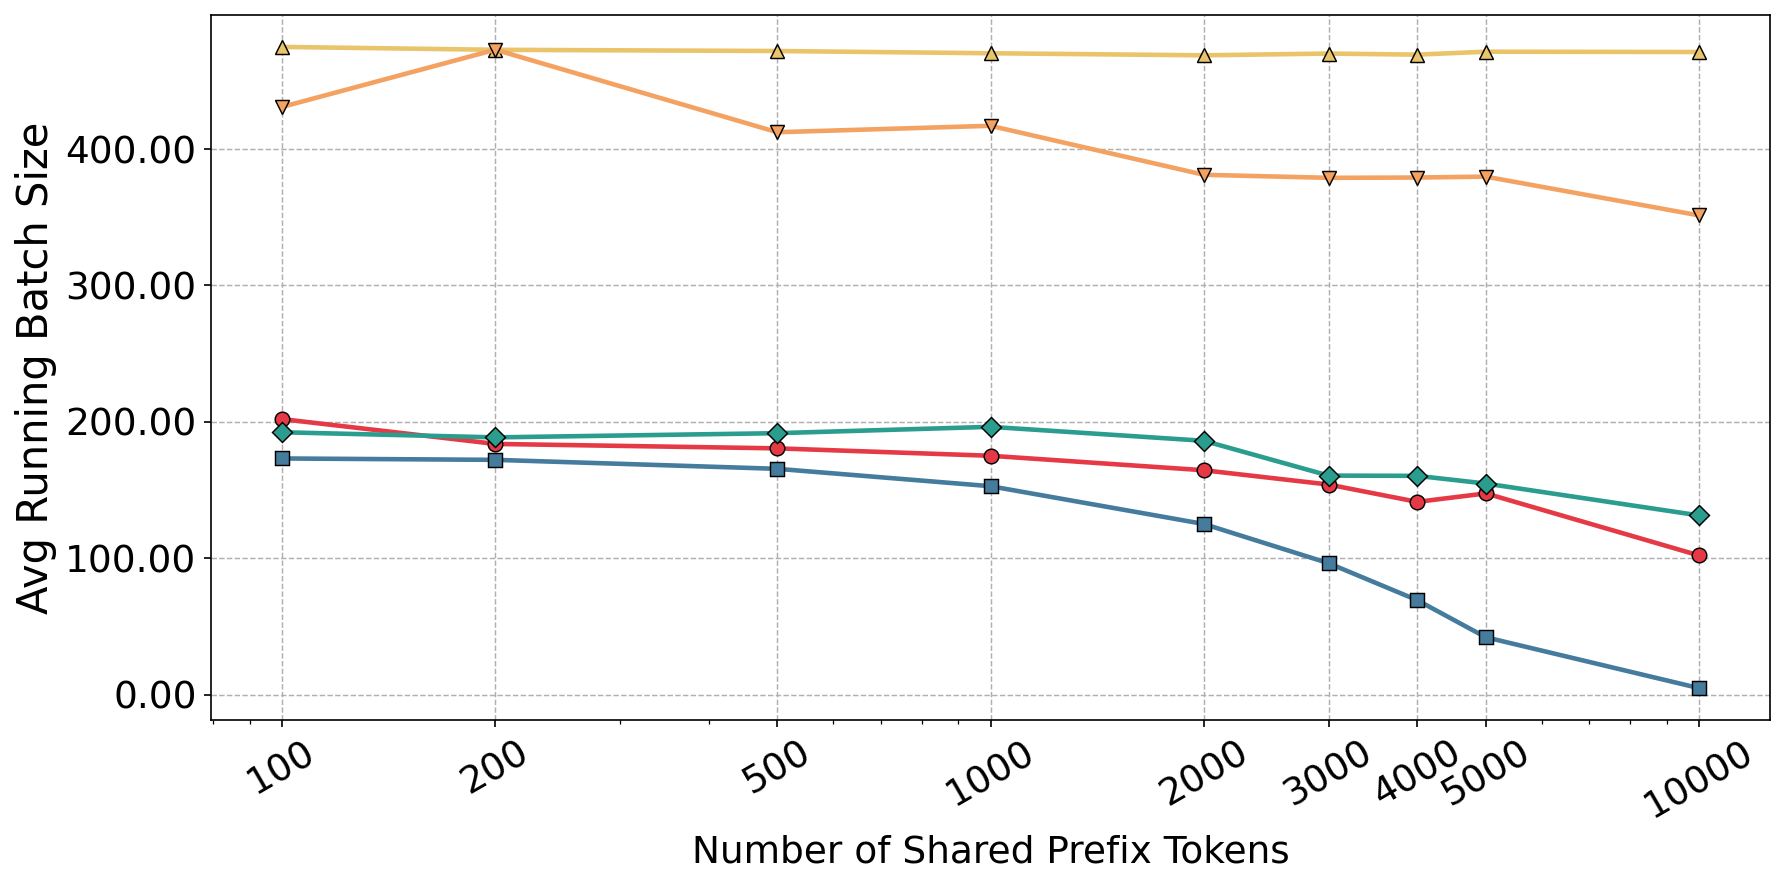
\includegraphics[width=\linewidth]{results/sys_prompt_tokens_plots/avg_batch_vs_sys_prompt_tokens.png}
    \caption{}
    \label{fig:tbt_vs_sys}
\end{subfigure}
\hfill
\begin{subfigure}{0.32\textwidth}
    \centering
    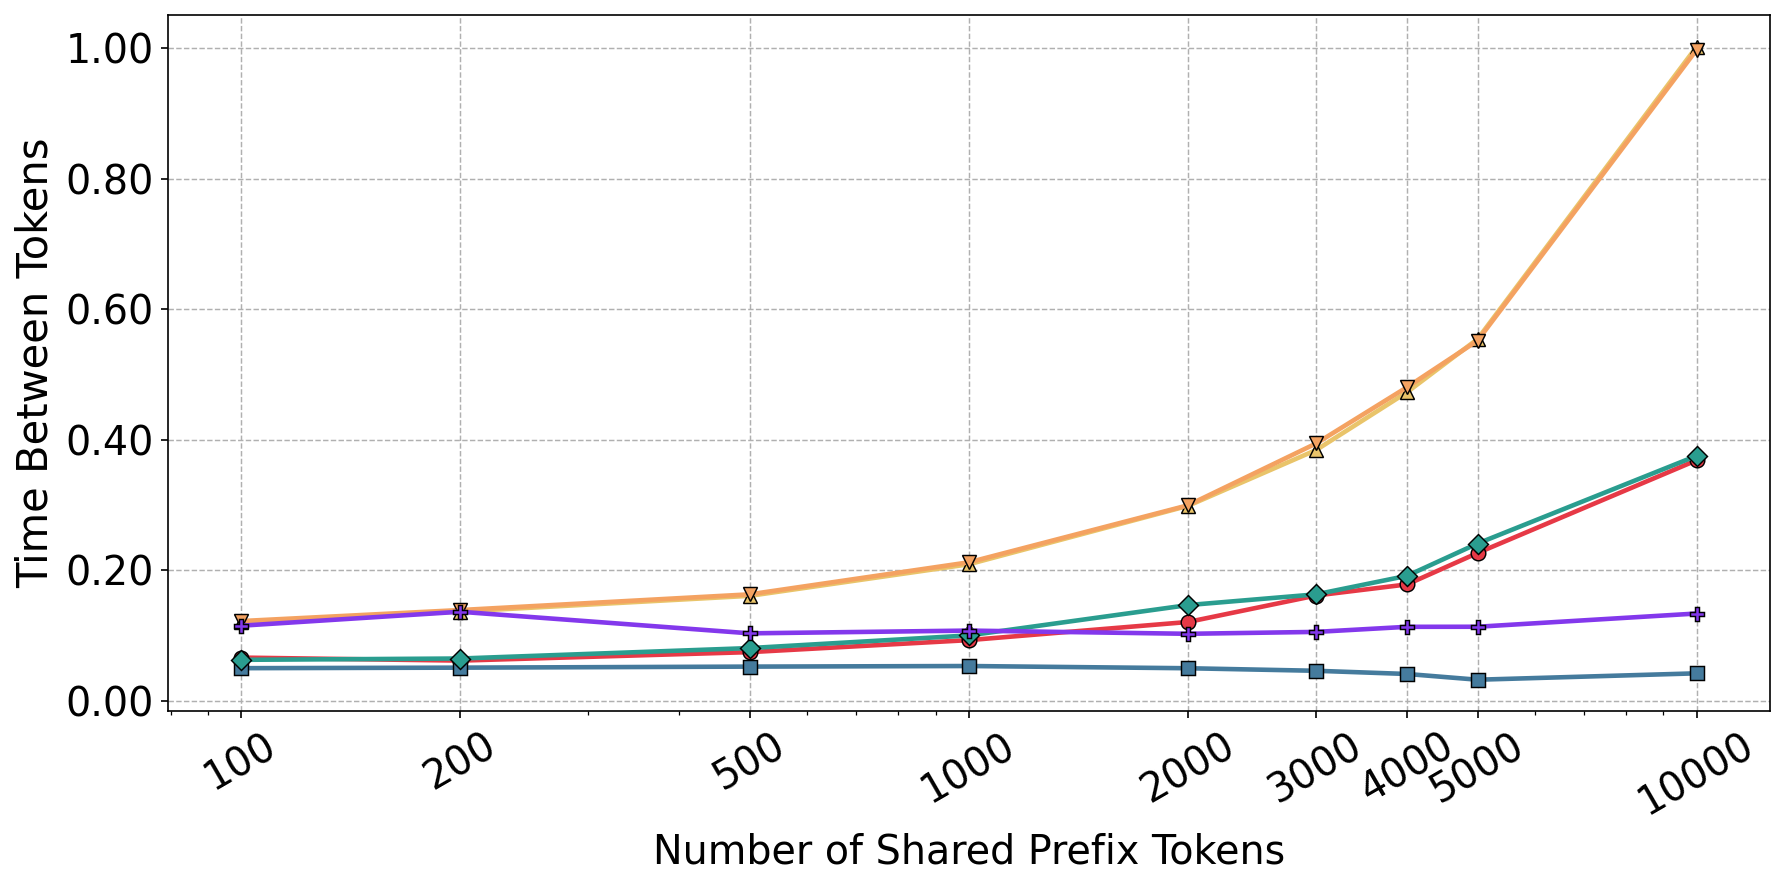
\includegraphics[width=\linewidth]{results/sys_prompt_tokens_plots/avg_timediff_vs_sys_prompt_tokens.png}
    \caption{}
    \label{fig:abs_vs_sys}
\end{subfigure}

\caption{Various metrics across varying number of shared prefix tokens. 200 tokens decode length; 500 input request poisson rate and 5 prefix groups.}
\label{fig:metrics_vs_sys}
\end{figure*}

\textcolor{red}{add many more results - on TBT, normalized latency, out tokens/sec?}



\section{Conclusion}
\label{sec:conclusion}


\bibliographystyle{ACM-Reference-Format}
\bibliography{references}

\appendix


\clearpage

\section{Algorithms}



\section{Throughput vs Batch Size for small requests with no prefix shared}
\begin{figure}[H]
\centering
\begin{minipage}{1\columnwidth}
\centering
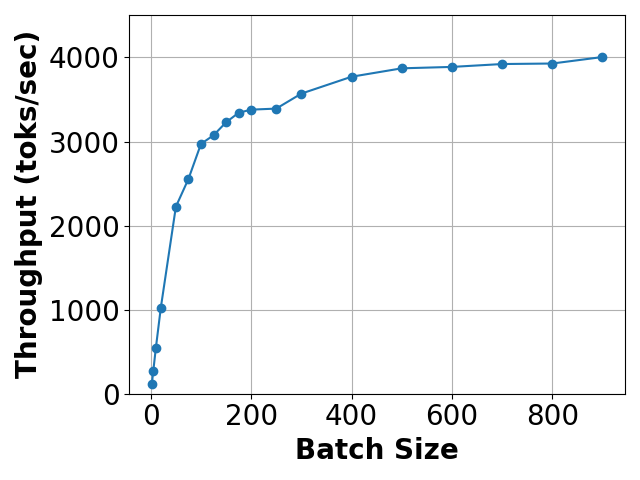
\includegraphics[width=\columnwidth]{results/throughput_vs_batch_size_llama8b_small_requests.png}
\caption{Throughput vs Batch Size}
\label{fig:batch_size_tp}
\end{minipage}
\hfill
\begin{minipage}{1\columnwidth}
\centering
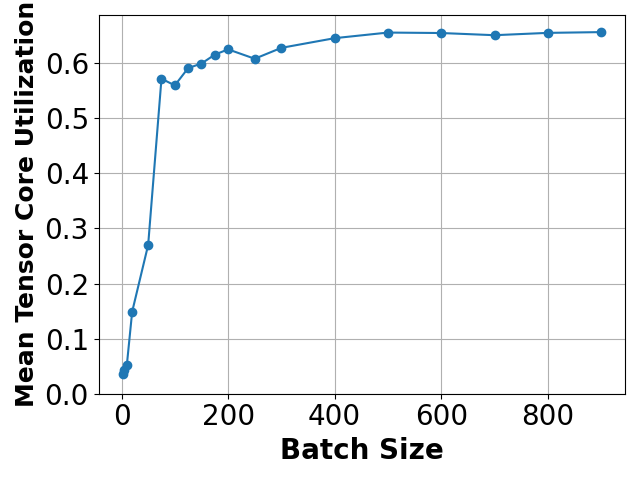
\includegraphics[width=\columnwidth]{results/mean_tenso_vs_batch_size_llama8b_small_requests.png}
\caption{Tensor Core Utilization vs Batch Size}
\label{fig:batch_size_tenso}
\end{minipage}
\hfill
\begin{minipage}{1\columnwidth}
\centering
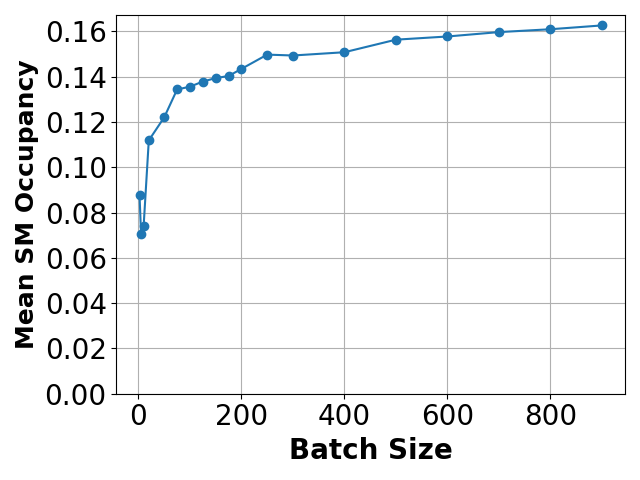
\includegraphics[width=\columnwidth]{results/mean_smocc_vs_batch_size_llama8b_small_requests.png}
\caption{Mean SM Occupancy vs Batch Size}
\label{fig:batch_size_tenso}
\end{minipage}
\end{figure}
\section{Impact of Sharing Position on Decode Throughput - $5L$}


\textcolor{orange}{To further strengthen our observations, we also present results for a sequence length of $5L$ in Figure~\ref{fig:tp_vs_l_1_9_11_5L}, where we extend the length of the top shared nodes by $L$ for all of these settings (the no sharing patterns remain unchanged, with both prefix groups of length $5L$ each).} \textcolor{red}{plot in appendix, but do we need this here?}
\begin{figure}[H]
\centering
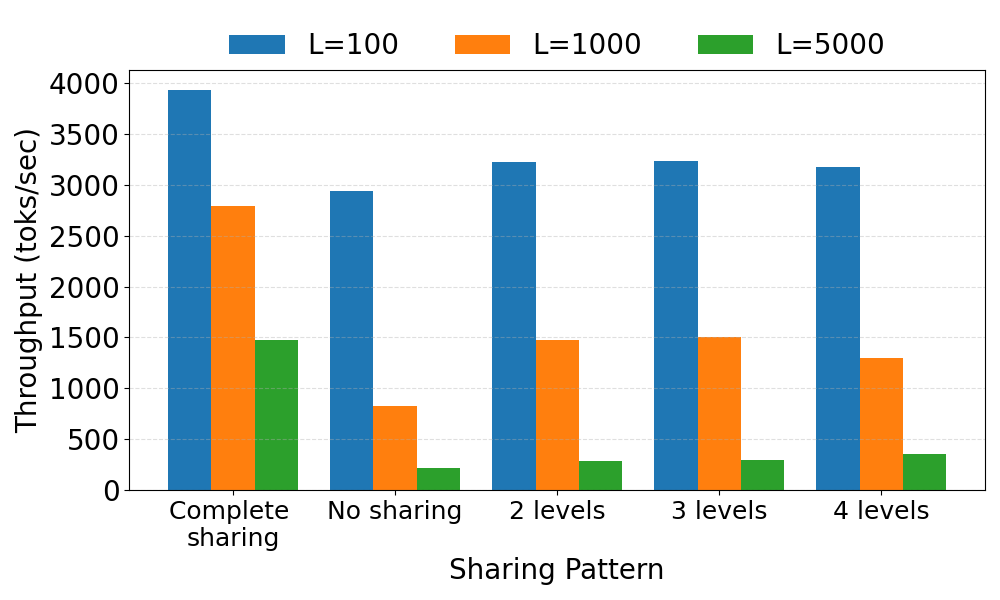
\includegraphics[width=\columnwidth]{results/tp_different_modes_sharing_at_top_5L.png}
\caption{Throughput vs sharing patterns}
\label{fig:tp_vs_l_1_9_11_5L}
\end{figure}


\section{Homo vs Hetero - No Warmup - Varying Decode Tokens}
\label{sec:homo_hetero_no_warmup}

\begin{figure}[H]
\centering
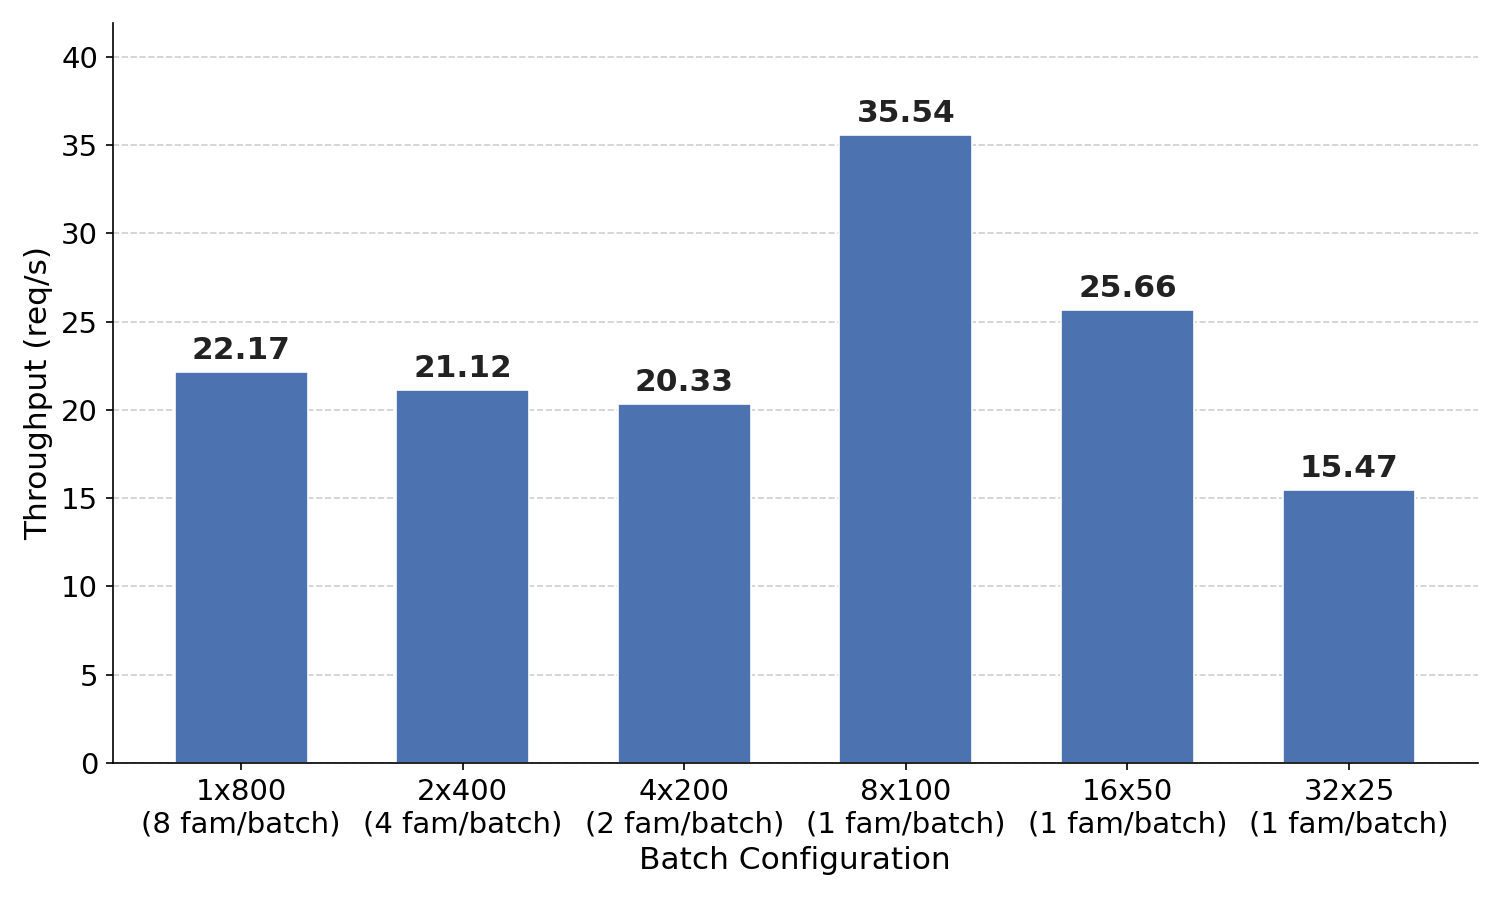
\includegraphics[width=0.8\columnwidth]{results/homo_hetero_throughput_barchart.png}
\caption{with warmup - 50 decode tokens}
\label{fig:homo_hetero_tp_001}
\end{figure}


\begin{figure}[H]
\centering
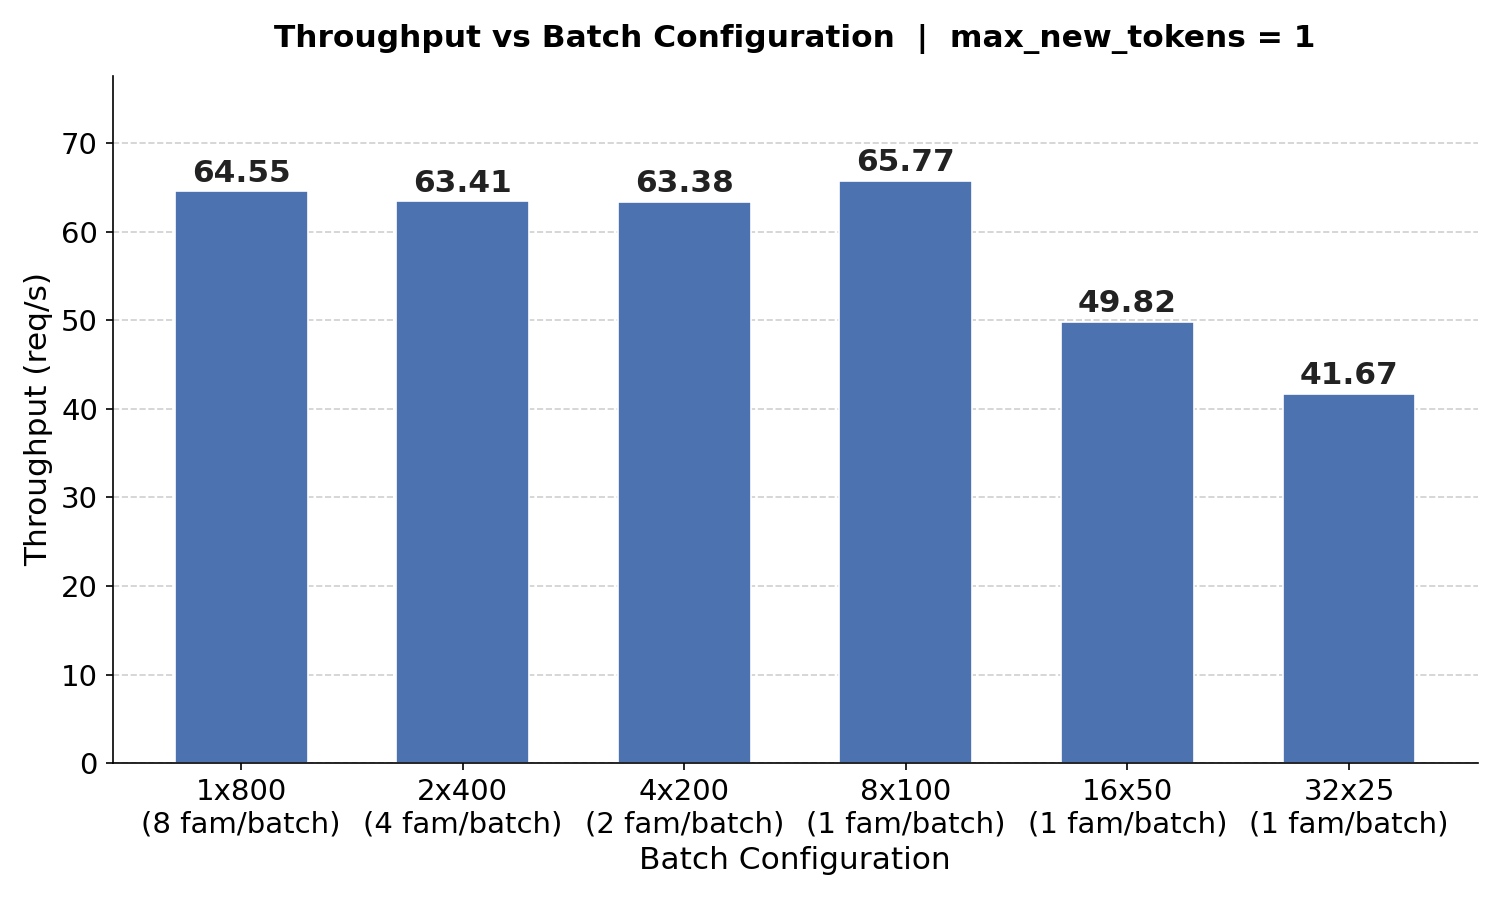
\includegraphics[width=0.8\columnwidth]{results/homo_hetero_throughput_barchart_no_warmup_tok001.png}
\caption{Throughput vs Batch Configuration}
\label{fig:homo_hetero_tp_001}
\end{figure}


\begin{figure}[H]
\centering
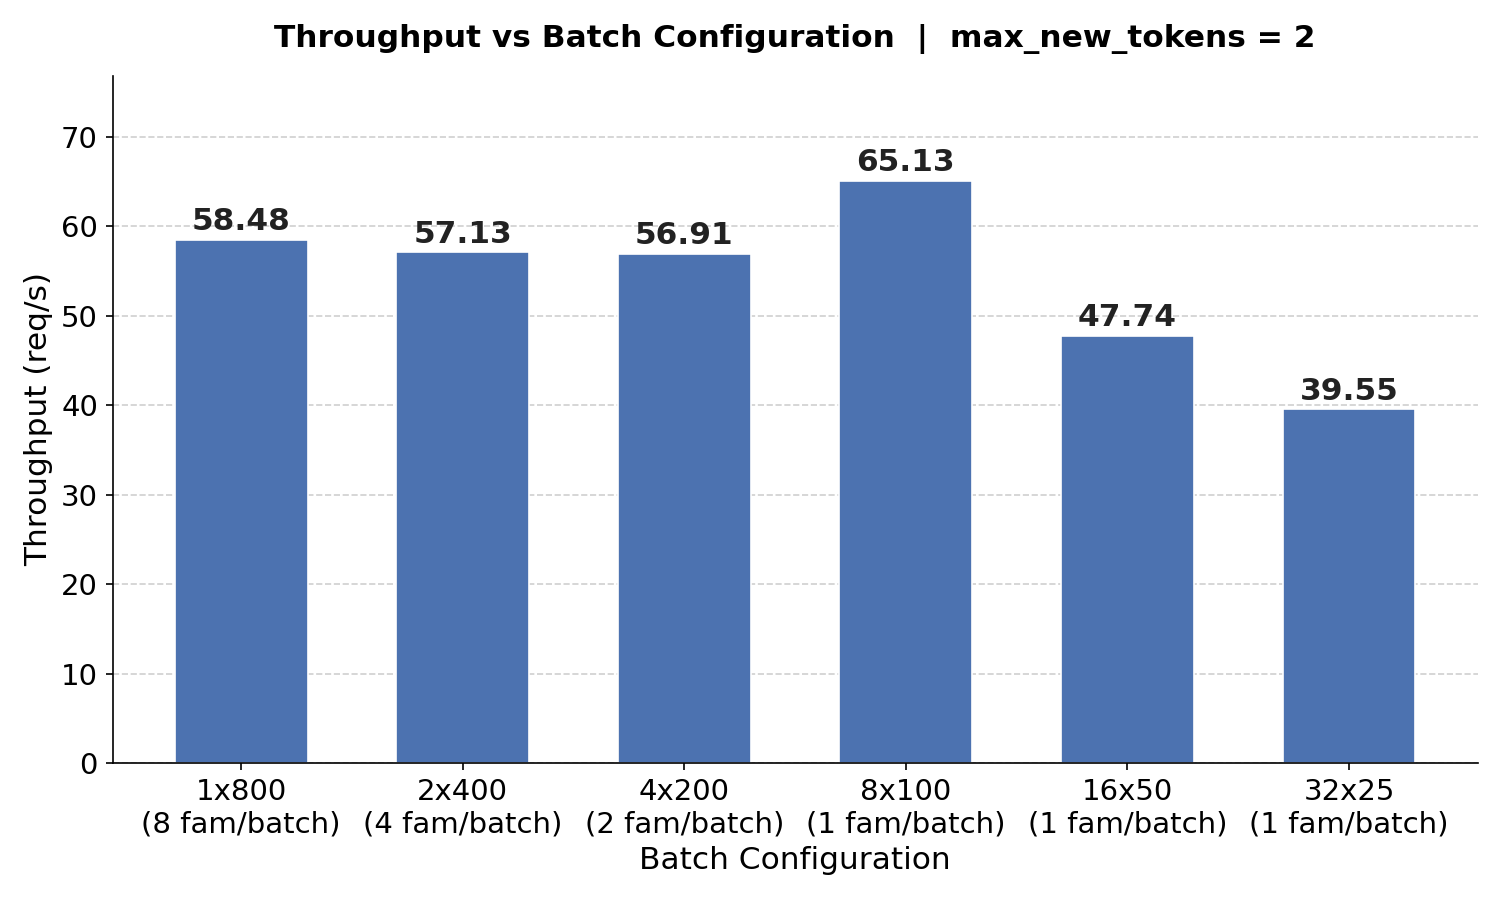
\includegraphics[width=0.8\columnwidth]{results/homo_hetero_throughput_barchart_no_warmup_tok002.png}
\caption{Throughput vs Batch Configuration}
\label{fig:homo_hetero_tp_002}
\end{figure}

\begin{figure}[H]
\centering
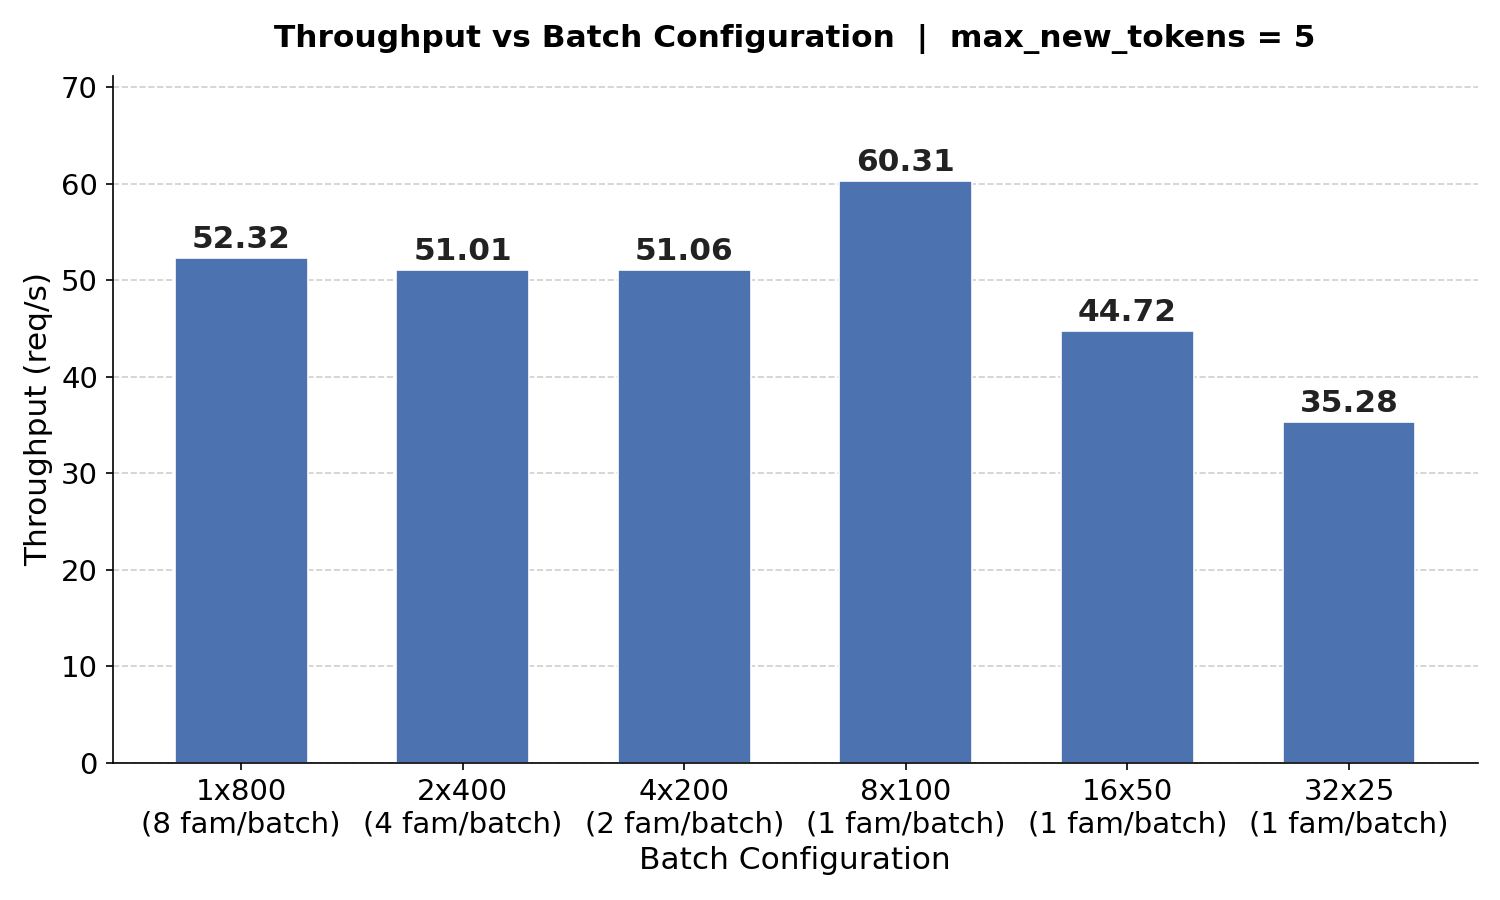
\includegraphics[width=0.8\columnwidth]{results/homo_hetero_throughput_barchart_no_warmup_tok005.png}
\caption{Throughput vs Batch Configuration}
\label{fig:homo_hetero_tp_005}
\end{figure}

\begin{figure}[H]
\centering
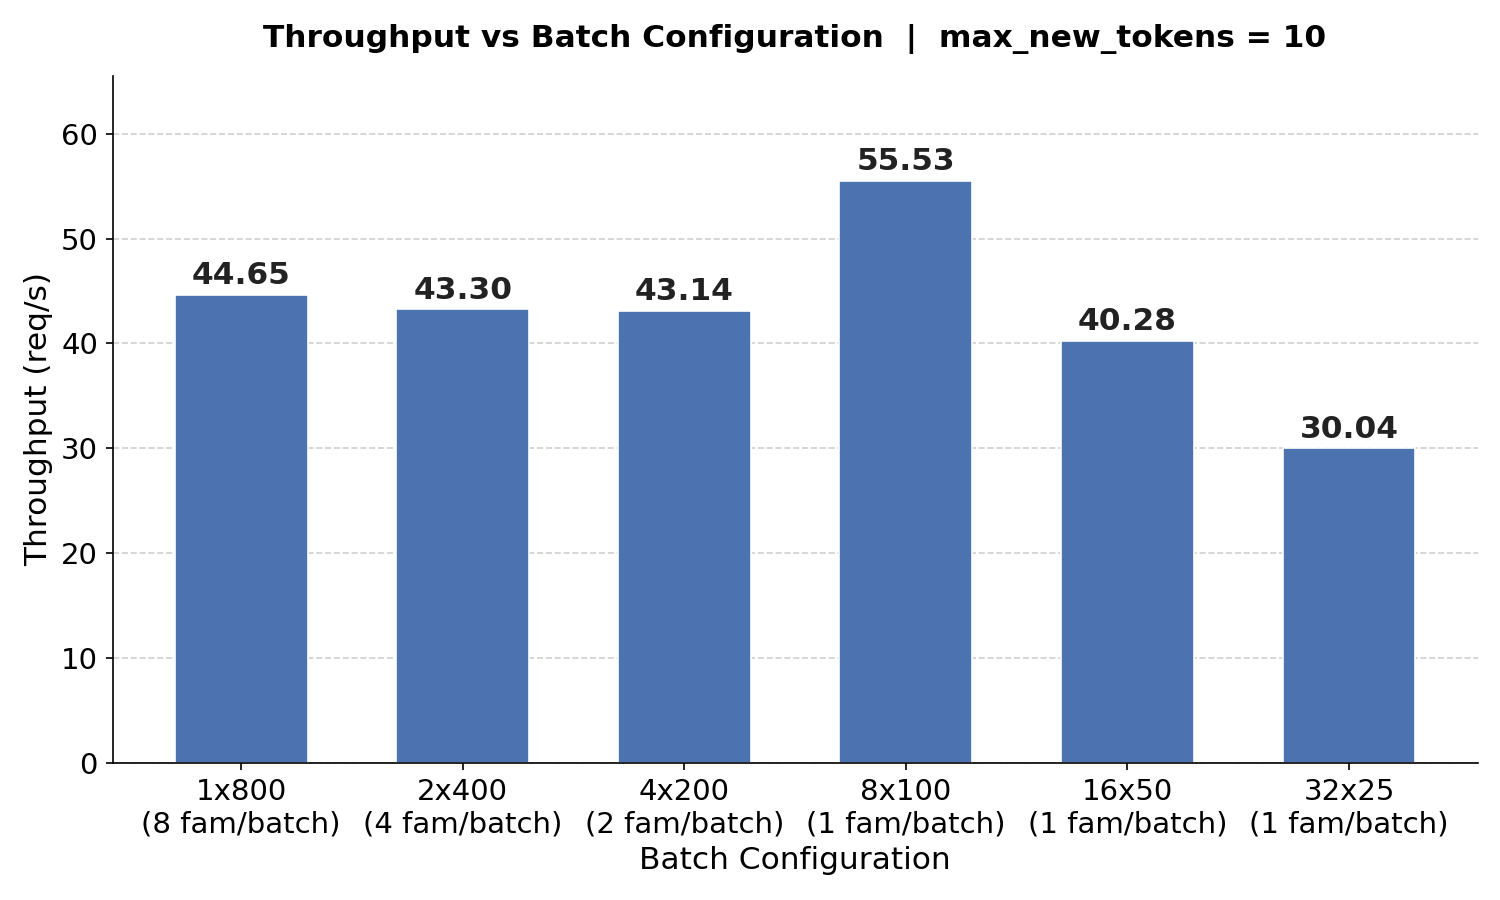
\includegraphics[width=0.8\columnwidth]{results/homo_hetero_throughput_barchart_no_warmup_tok010.png}
\caption{Throughput vs Batch Configuration}
\label{fig:homo_hetero_tp_010}
\end{figure}

\begin{figure}[H]
\centering
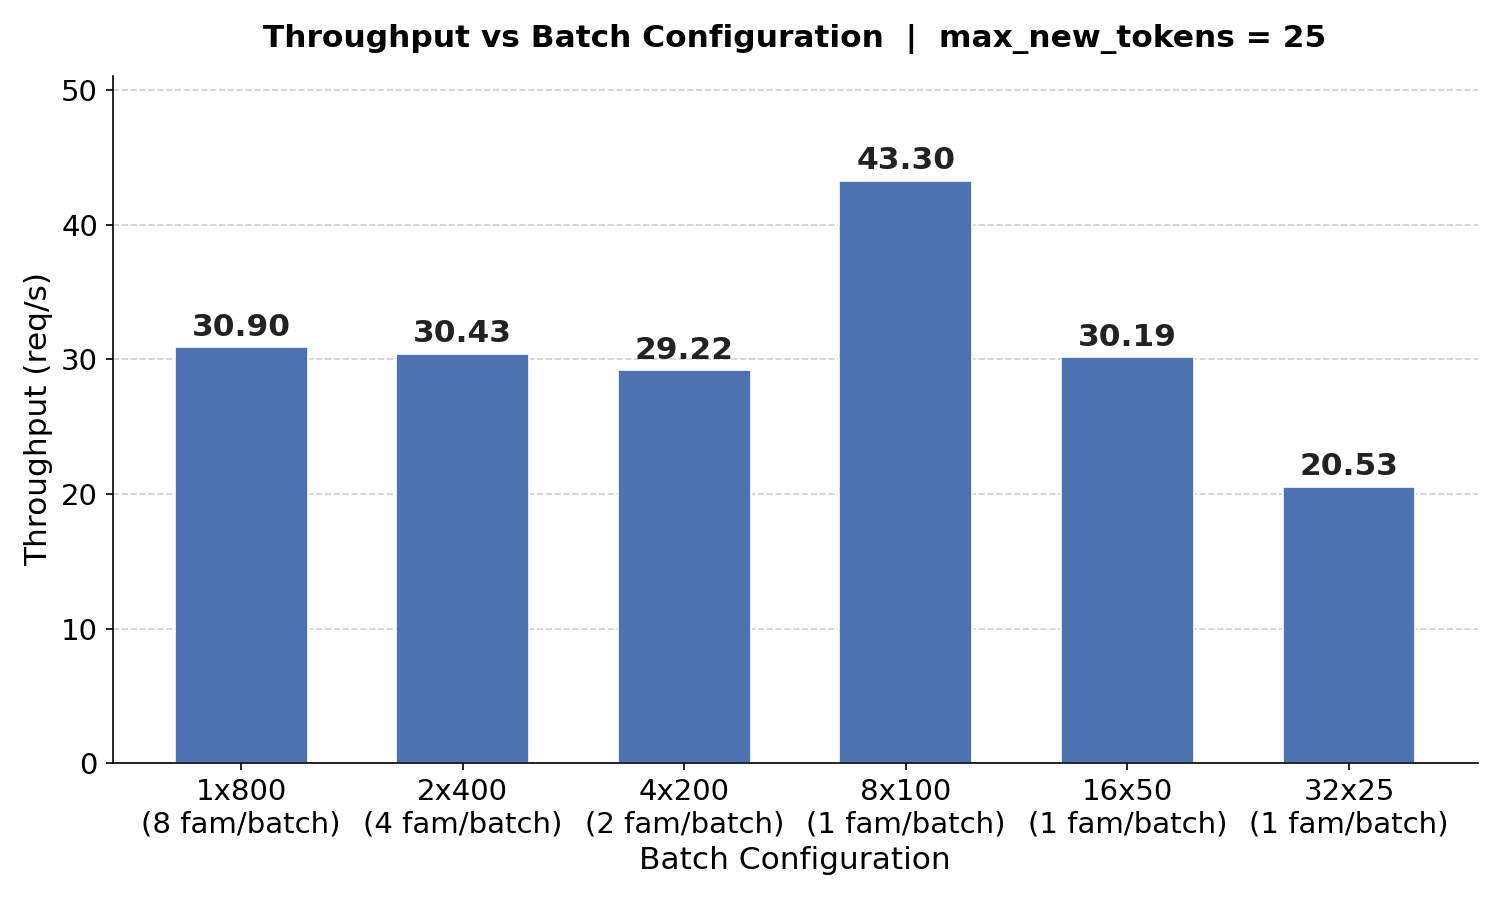
\includegraphics[width=0.8\columnwidth]{results/homo_hetero_throughput_barchart_no_warmup_tok025.png}
\caption{Throughput vs Batch Configuration}
\label{fig:homo_hetero_tp_025}
\end{figure}

\begin{figure}[H]
\centering
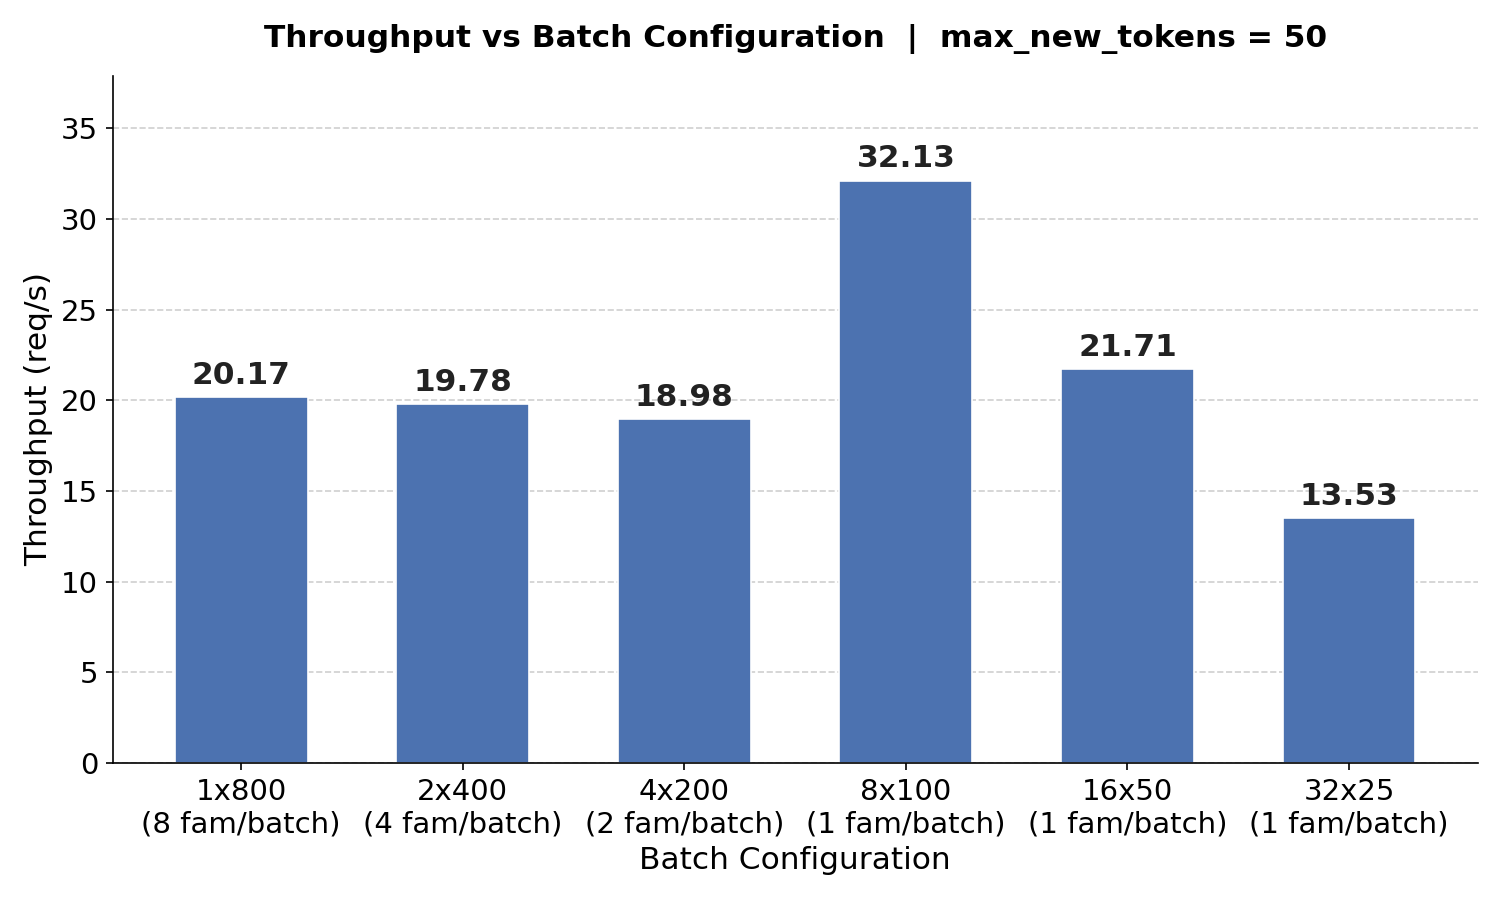
\includegraphics[width=0.8\columnwidth]{results/homo_hetero_throughput_barchart_no_warmup_tok050.png}
\caption{Throughput vs Batch Configuration}
\label{fig:homo_hetero_tp_050}
\end{figure}

\begin{figure}[H]
\centering
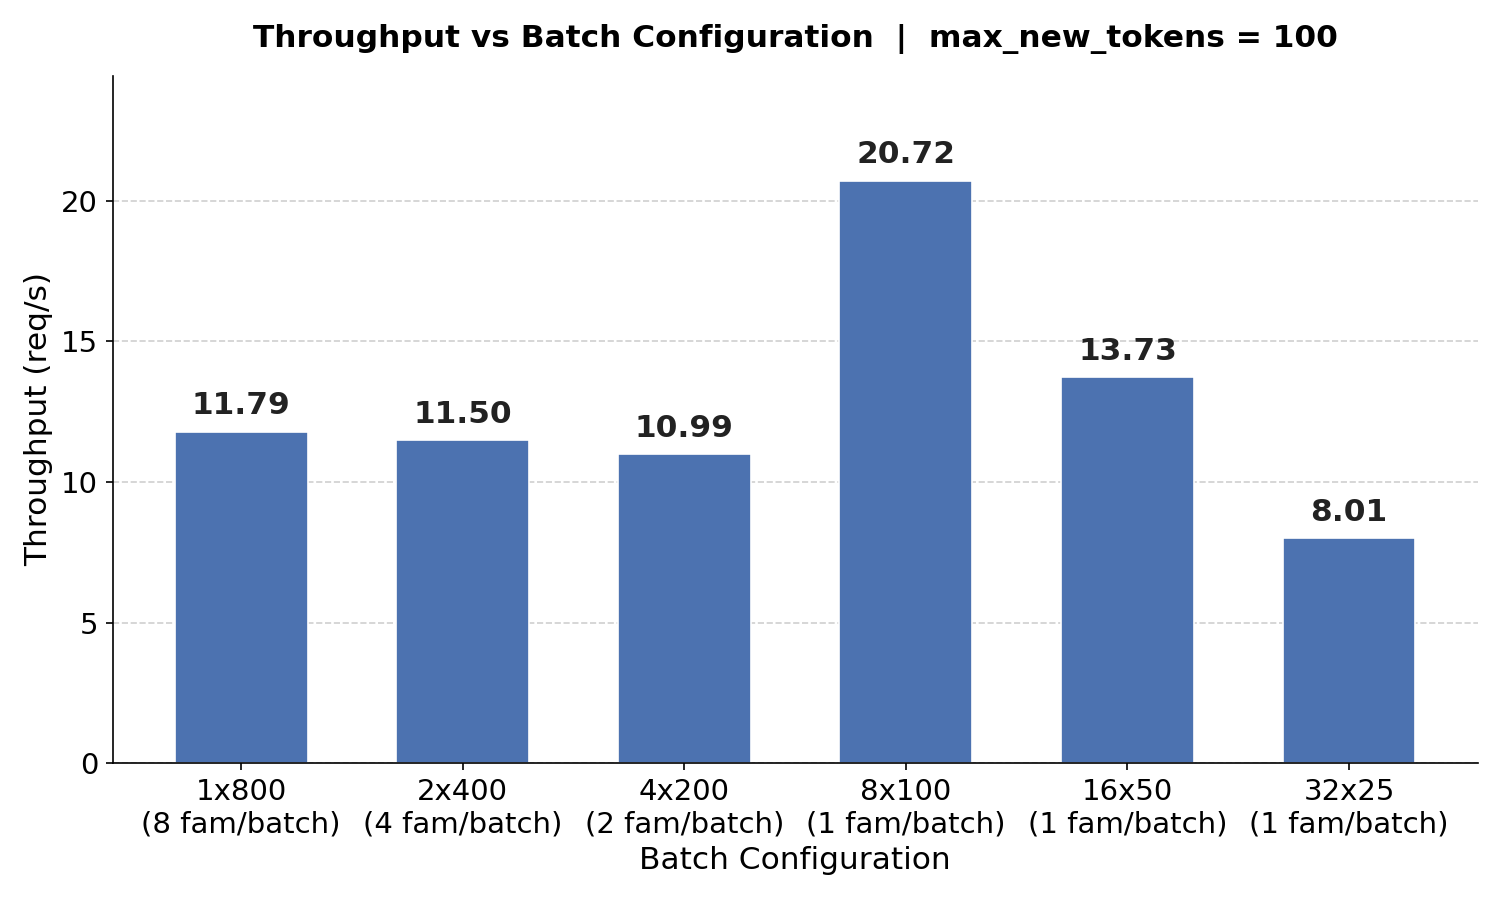
\includegraphics[width=0.8\columnwidth]{results/homo_hetero_throughput_barchart_no_warmup_tok100.png}
\caption{Throughput vs Batch Configuration}
\label{fig:homo_hetero_tp_100}
\end{figure}

\begin{figure}[H]
\centering
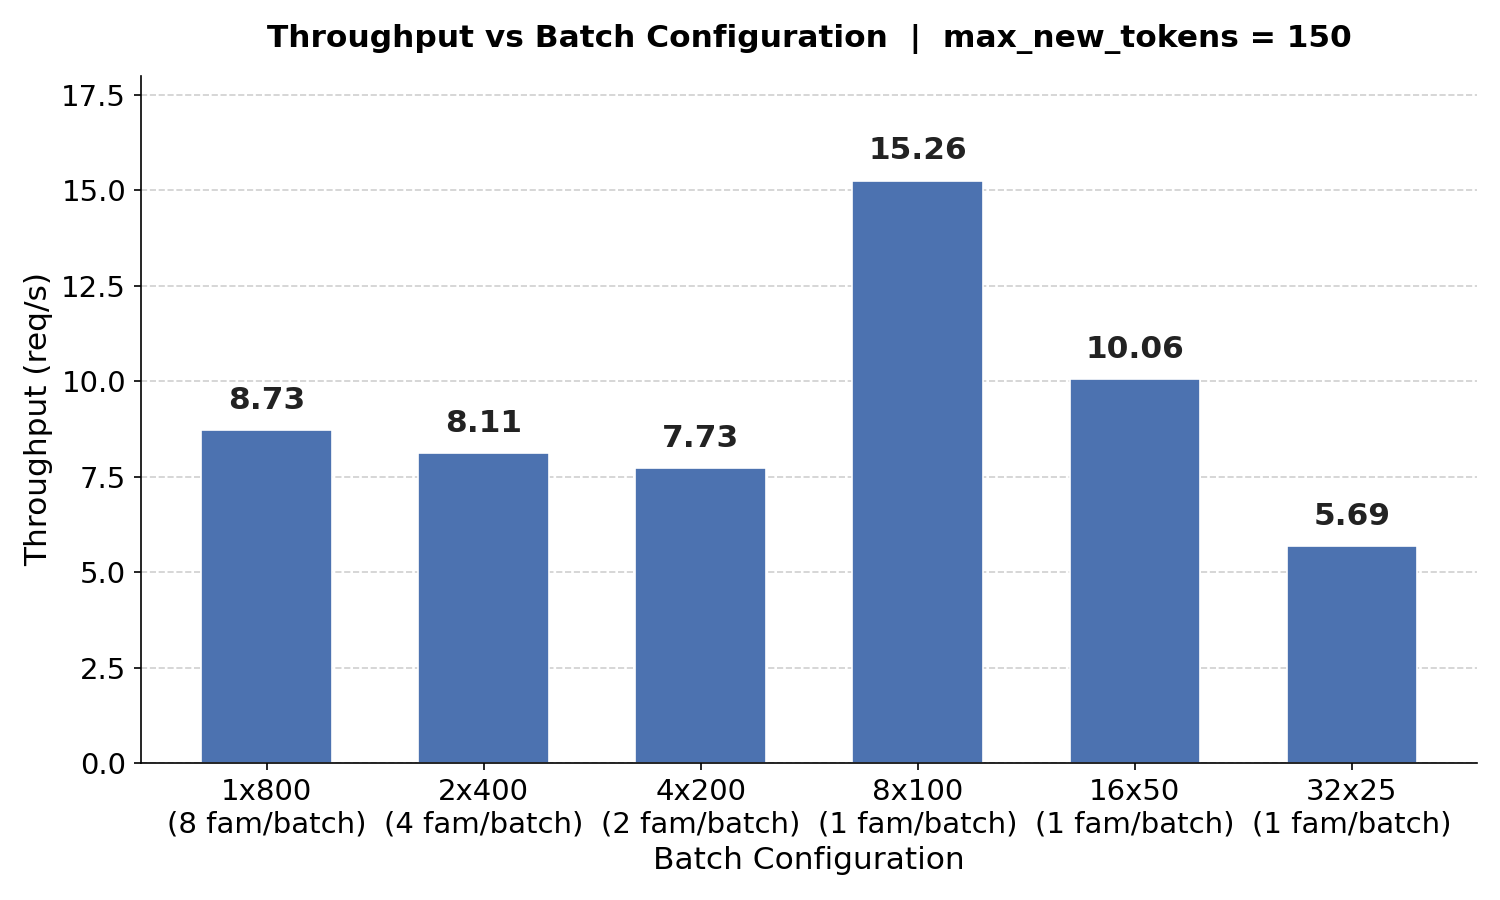
\includegraphics[width=0.8\columnwidth]{results/homo_hetero_throughput_barchart_no_warmup_tok150.png}
\caption{Throughput vs Batch Configuration}
\label{fig:homo_hetero_tp_150}
\end{figure}

\begin{figure}[H]
\centering
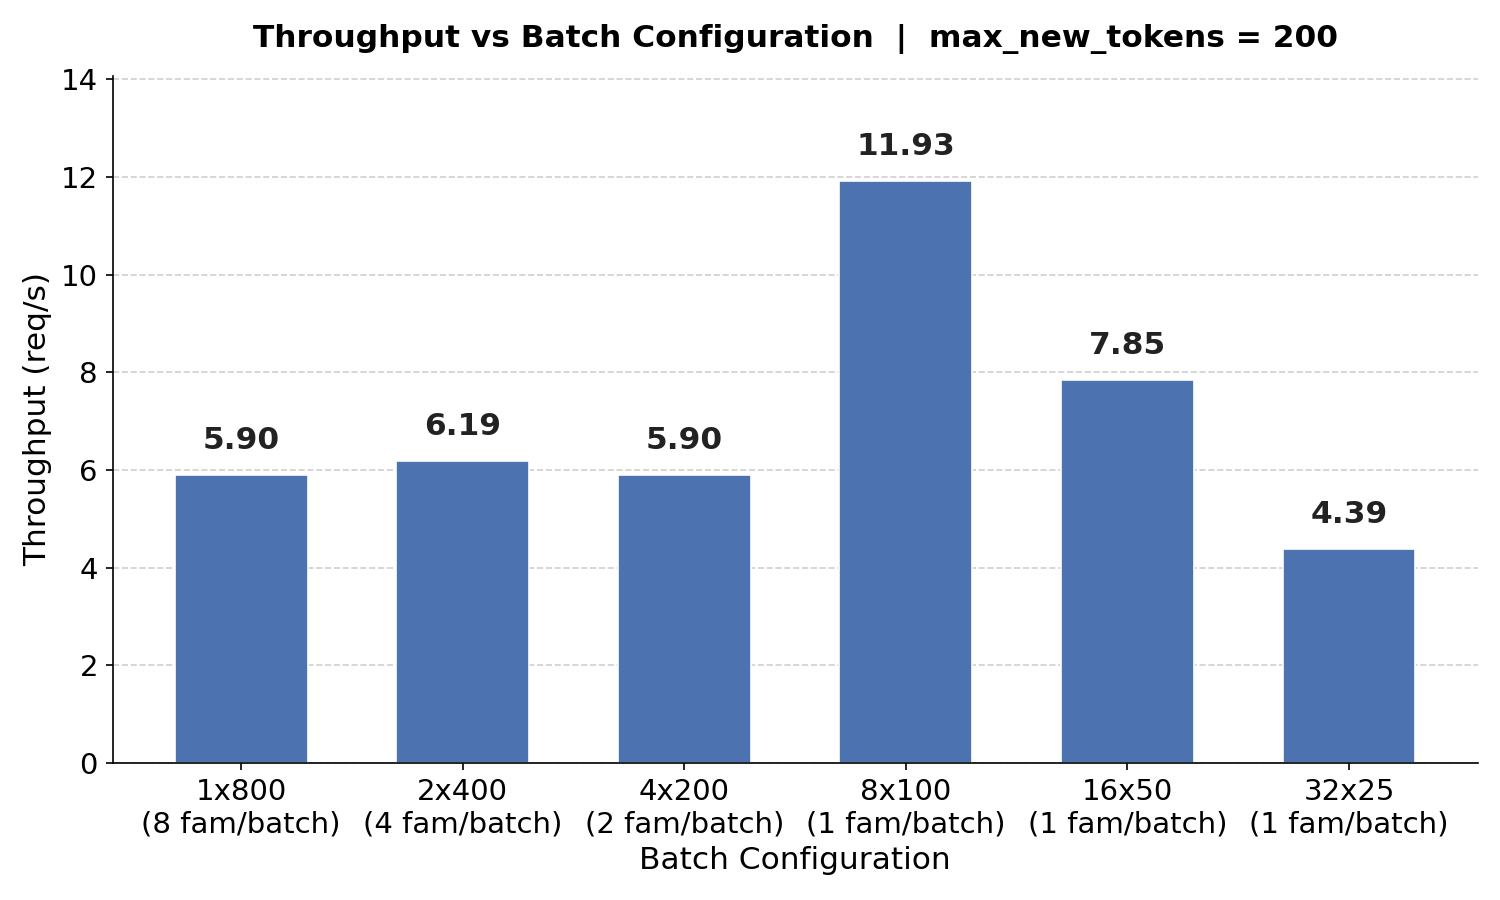
\includegraphics[width=0.8\columnwidth]{results/homo_hetero_throughput_barchart_no_warmup_tok200.png}
\caption{Throughput vs Batch Configuration}
\label{fig:homo_hetero_tp_200}
\end{figure}

\begin{figure}[H]
\centering
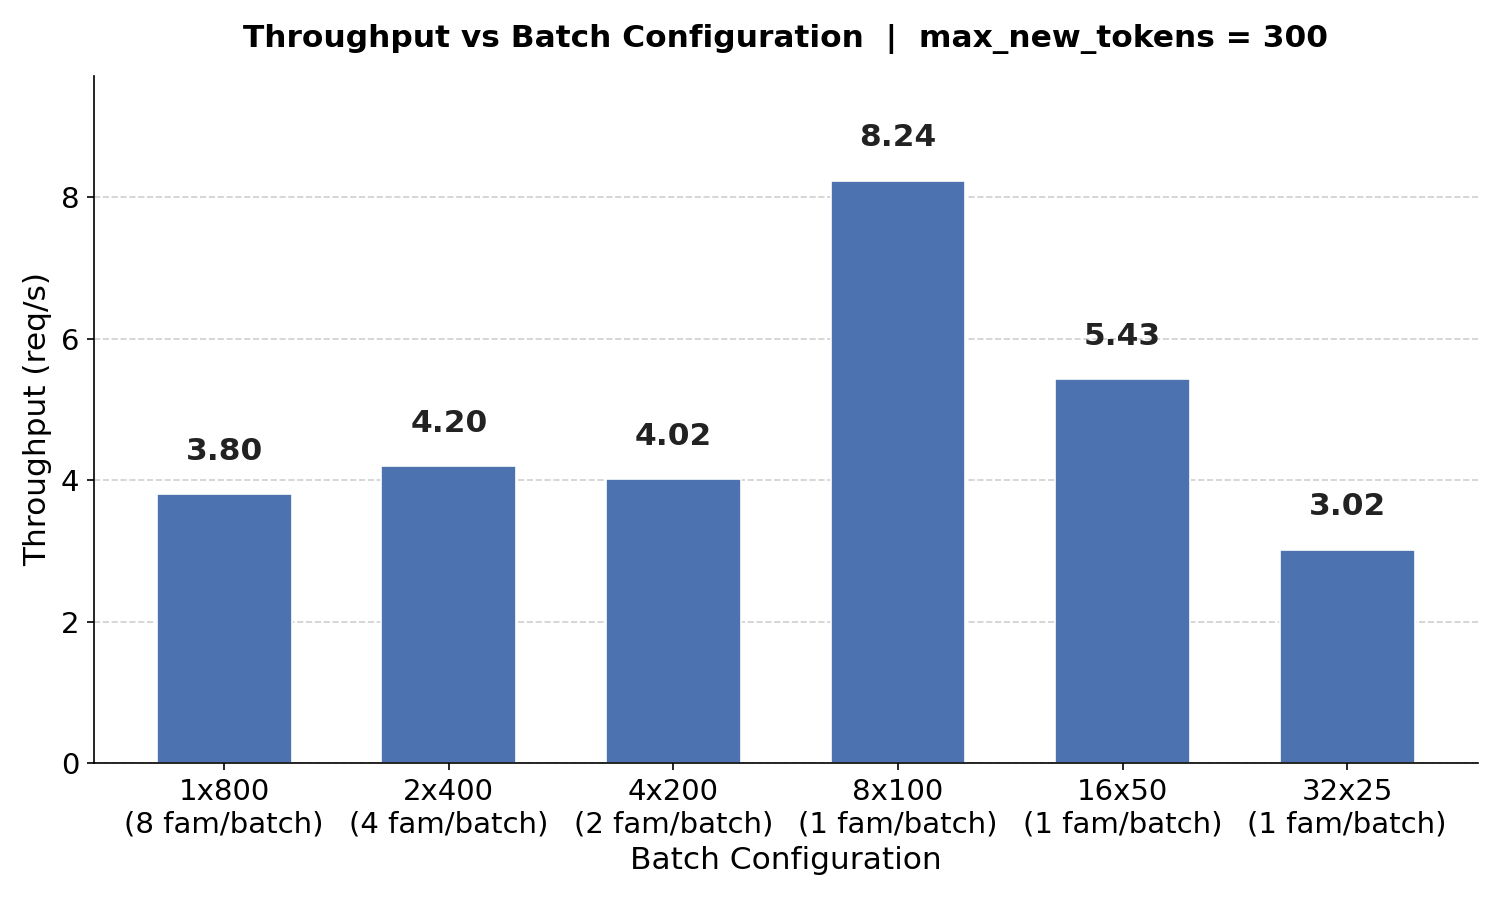
\includegraphics[width=0.8\columnwidth]{results/homo_hetero_throughput_barchart_no_warmup_tok300.png}
\caption{Throughput vs Batch Configuration}
\label{fig:homo_hetero_tp_300}
\end{figure}


\section{Mean SM Occupancy vs Batch Size}
\begin{figure}[H]
\centering
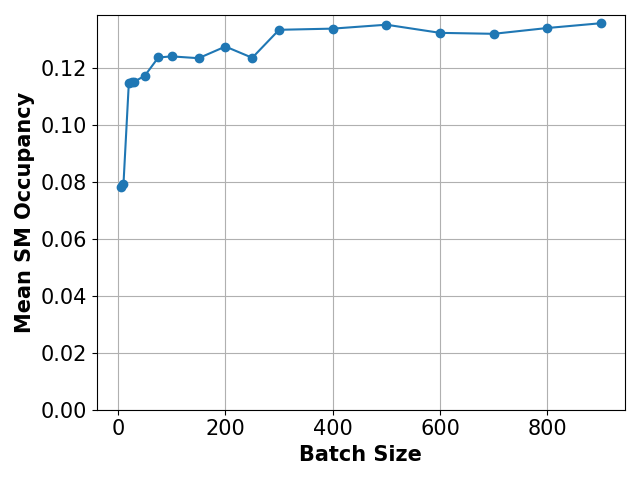
\includegraphics[width=\columnwidth]{results/mean_smocc_vs_batch_size_llama8b.png}
\caption{SM Occupancy}
\label{fig:batch_size_smocc}
\end{figure}

\section{Cache Working Set Size Theory}
\begin{figure}[H]
\centering
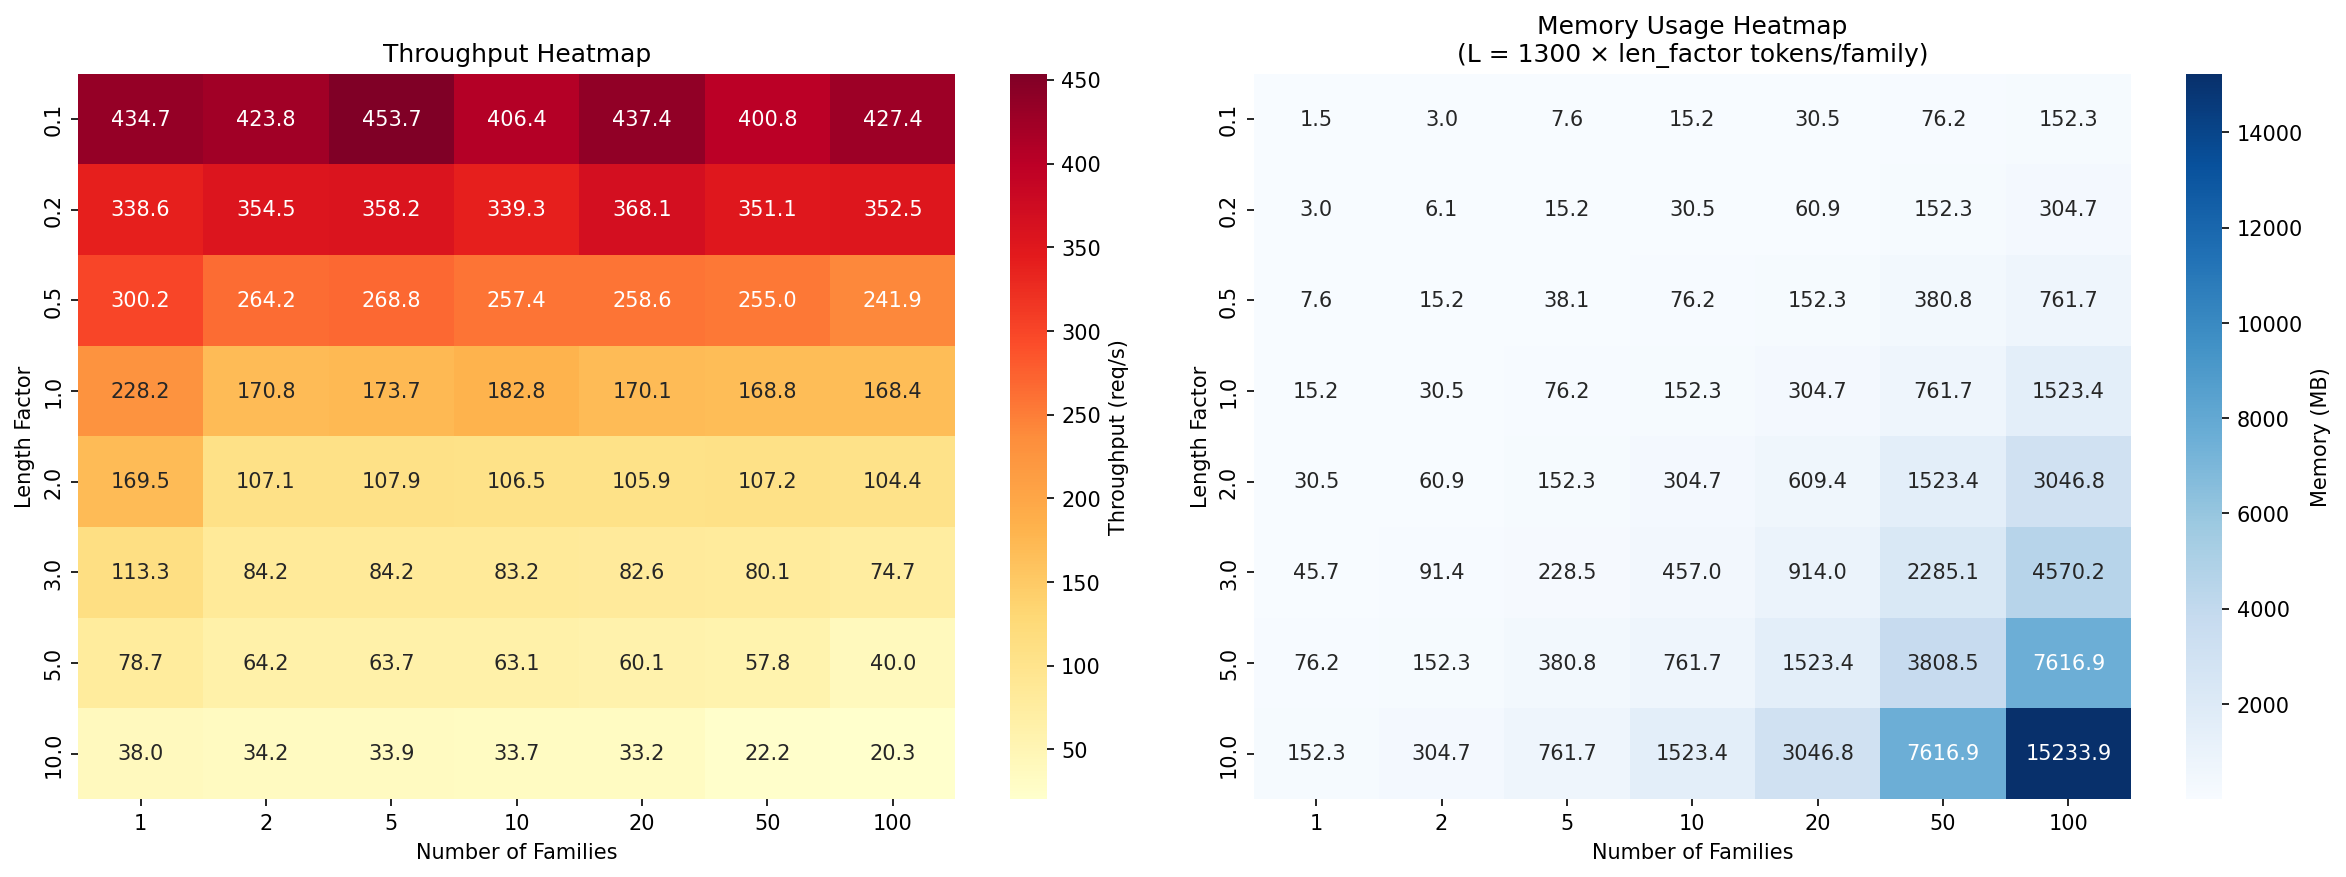
\includegraphics[width=\columnwidth]{results/qwen_families_lengths_tp_mem.png}
\caption{QWEN Throughput and KV Cache Memory across various sequence lengths and number of families}
\label{fig:qwen_fam_len_tp_mem}
\end{figure}



\newpage
\textcolor{red}{\LARGE DUMP APPENDIX STARTS HERE!!!}
\section{Radix Tree Workload Modes}

    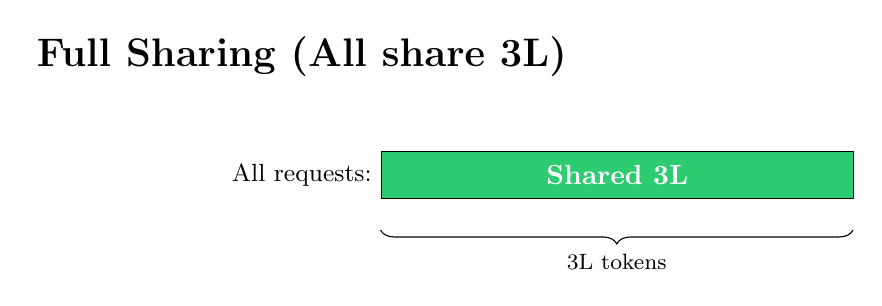
\begin{tikzpicture}[
    box/.style={rectangle, draw, minimum width=1cm, minimum height=0.6cm, anchor=west},
    label/.style={font=\small}
]
    \node[font=\Large\bfseries] at (0,2) {Full Sharing (All share 3L)};
    
    \node[label] at (0,0.5) {All requests:};
    
    \node[box, fill=shared1, minimum width=6cm] (s1) at (1,0.5) {};
    \node[label, white, font=\bfseries] at (s1.center) {Shared 3L};
    
    \draw[decorate, decoration={brace, amplitude=5pt, mirror}] 
        (1,-0.2) -- (7,-0.2) node[midway, below=5pt, font=\footnotesize] {3L tokens};
\end{tikzpicture}

    \hspace*{+1cm}
    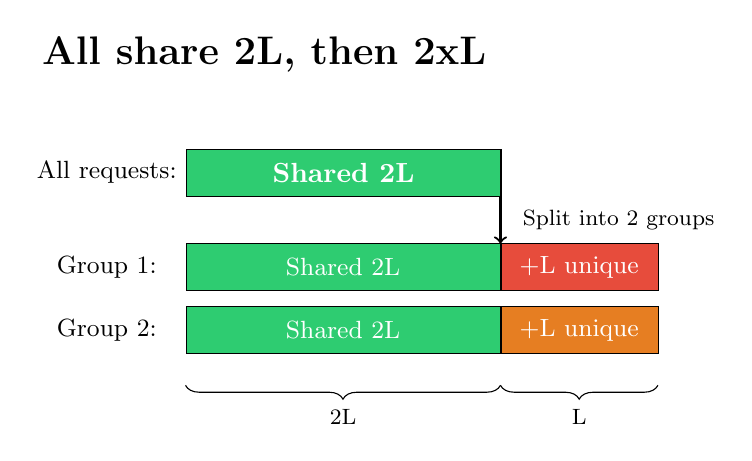
\begin{tikzpicture}[
    box/.style={rectangle, draw, minimum width=1cm, minimum height=0.6cm, anchor=west},
    label/.style={font=\small}
]
    \node[font=\Large\bfseries] at (2,3.5) {All share 2L, then 2xL};
    
    % Level 1: All share
    \node[label] at (0,2) {All requests:};
    \node[box, fill=shared1, minimum width=4cm] (l1) at (1,2) {};
    \node[label, white, font=\bfseries] at (l1.center) {Shared 2L};
    
    % Level 2: Two groups
    \node[label] at (0,0.8) {Group 1:};
    \node[box, fill=shared1, minimum width=4cm] at (1,0.8) {};
    \node[box, fill=unique1, minimum width=2cm] at (5,0.8) {};
    \node[label, white] at (3,0.8) {Shared 2L};
    \node[label, white] at (6,0.8) {+L unique};
    
    \node[label] at (0,0) {Group 2:};
    \node[box, fill=shared1, minimum width=4cm] at (1,0) {};
    \node[box, fill=unique2, minimum width=2cm] at (5,0) {};
    \node[label, white] at (3,0) {Shared 2L};
    \node[label, white] at (6,0) {+L unique};
    
    % Annotations
    \draw[decorate, decoration={brace, amplitude=5pt, mirror}] 
        (1,-0.7) -- (5,-0.7) node[midway, below=5pt, font=\footnotesize] {2L};
    \draw[decorate, decoration={brace, amplitude=5pt, mirror}] 
        (5,-0.7) -- (7,-0.7) node[midway, below=5pt, font=\footnotesize] {L};
    
    % Arrow showing split
    \draw[->, thick] (5,1.7) -- (5,1.1);
    \node[font=\footnotesize] at (6.5,1.4) {Split into 2 groups};
    
\end{tikzpicture}


    \hspace*{0cm}
    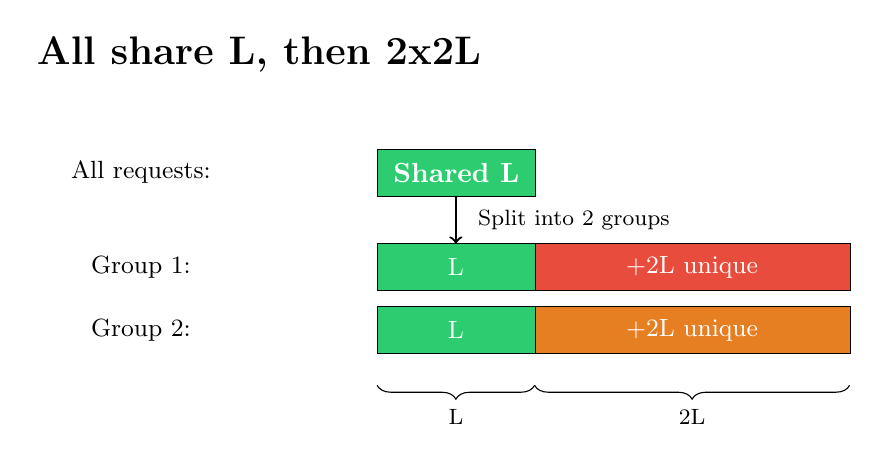
\begin{tikzpicture}[
    box/.style={rectangle, draw, minimum width=1cm, minimum height=0.6cm, anchor=west},
    label/.style={font=\small}
]
    \node[font=\Large\bfseries] at (1.5,3.5) {All share L, then 2x2L};
    
    \node[label] at (0,2) {All requests:};
    \node[box, fill=shared1, minimum width=2cm] (l1) at (3,2) {};
    \node[label, white, font=\bfseries] at (l1.center) {Shared L};
    
    \node[label] at (0,0.8) {Group 1:};
    \node[box, fill=shared1, minimum width=2cm] at (3,0.8) {};
    \node[box, fill=unique1, minimum width=4cm] at (5,0.8) {};
    \node[label, white] at (4,0.8) {L};
    \node[label, white] at (7,0.8) {+2L unique};
    
    \node[label] at (0,0) {Group 2:};
    \node[box, fill=shared1, minimum width=2cm] at (3,0) {};
    \node[box, fill=unique2, minimum width=4cm] at (5,0) {};
    \node[label, white] at (4,0) {L};
    \node[label, white] at (7,0) {+2L unique};
    
    \draw[decorate, decoration={brace, amplitude=5pt, mirror}] 
        (3,-0.7) -- (5,-0.7) node[midway, below=5pt, font=\footnotesize] {L};
    \draw[decorate, decoration={brace, amplitude=5pt, mirror}] 
        (5,-0.7) -- (9,-0.7) node[midway, below=5pt, font=\footnotesize] {2L};
    
    \draw[->, thick] (4,1.7) -- (4,1.1);
    \node[font=\footnotesize] at (5.5,1.4) {Split into 2 groups};
    
\end{tikzpicture}



    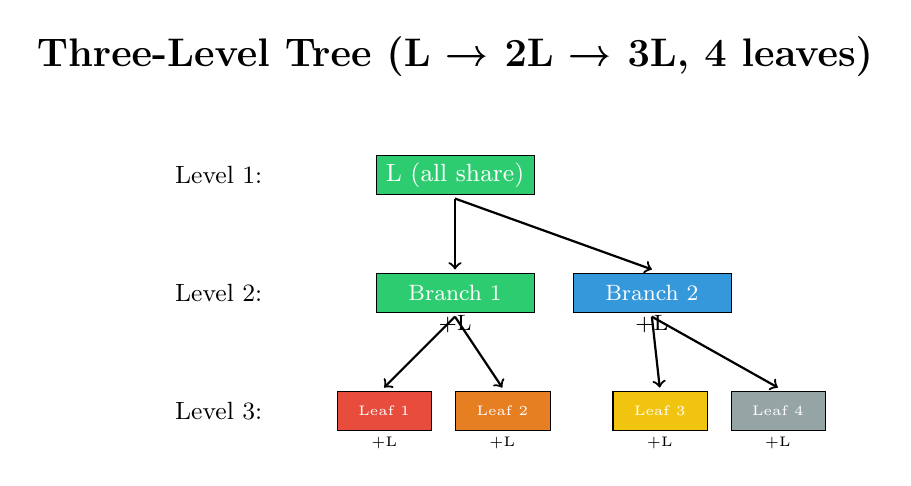
\begin{tikzpicture}[
    box/.style={rectangle, draw, minimum width=0.8cm, minimum height=0.5cm, anchor=west},
    label/.style={font=\small},
    level distance=1.2cm,
    level 1/.style={sibling distance=6cm},
    level 2/.style={sibling distance=3cm}
]
    \node[font=\Large\bfseries] at (3,5) {Three-Level Tree (L → 2L → 3L, 4 leaves)};
    
    \node[label] at (0,3.5) {Level 1:};
    \node[box, fill=shared1, minimum width=2cm] at (2,3.5) {};
    \node[label, white] at (3,3.5) {L (all share)};
    
    \node[label] at (0,2) {Level 2:};
    \node[box, fill=shared1, minimum width=2cm] at (2,2) {};
    \node[box, fill=shared2, minimum width=2cm] at (4.5,2) {};
    \node[label, white, font=\footnotesize] at (3,2) {Branch 1};
    \node[label, white, font=\footnotesize] at (5.5,2) {Branch 2};
    \node[font=\footnotesize] at (3,1.6) {+L};
    \node[font=\footnotesize] at (5.5,1.6) {+L};
    
    \node[label] at (0,0.5) {Level 3:};
    \node[box, fill=unique1, minimum width=1.2cm] at (1.5,0.5) {};
    \node[box, fill=unique2, minimum width=1.2cm] at (3,0.5) {};
    \node[box, fill=unique3, minimum width=1.2cm] at (5,0.5) {};
    \node[box, fill=unique4, minimum width=1.2cm] at (6.5,0.5) {};
    
    \node[label, white, font=\tiny] at (2.1,0.5) {Leaf 1};
    \node[label, white, font=\tiny] at (3.6,0.5) {Leaf 2};
    \node[label, white, font=\tiny] at (5.6,0.5) {Leaf 3};
    \node[label, white, font=\tiny] at (7.1,0.5) {Leaf 4};
    
    \node[font=\tiny] at (2.1,0.1) {+L};
    \node[font=\tiny] at (3.6,0.1) {+L};
    \node[font=\tiny] at (5.6,0.1) {+L};
    \node[font=\tiny] at (7.1,0.1) {+L};
    
    \draw[->, thick] (3,3.2) -- (3,2.3);
    \draw[->, thick] (3,3.2) -- (5.5,2.3);
    \draw[->, thick] (3,1.7) -- (2.1,0.8);
    \draw[->, thick] (3,1.7) -- (3.6,0.8);
    \draw[->, thick] (5.5,1.7) -- (5.6,0.8);
    \draw[->, thick] (5.5,1.7) -- (7.1,0.8);
\end{tikzpicture}


    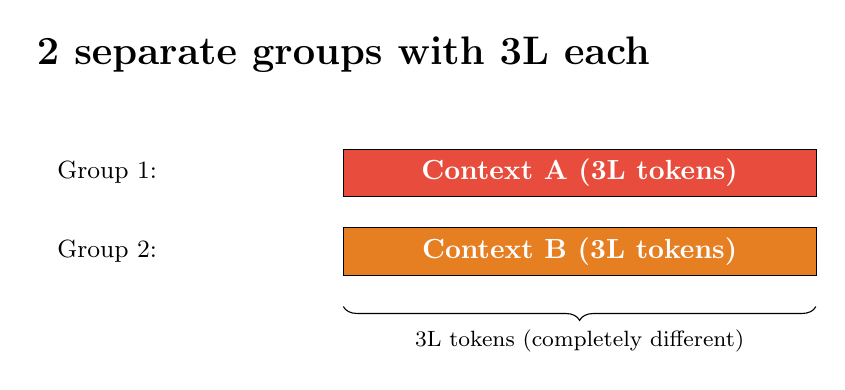
\begin{tikzpicture}[
    box/.style={rectangle, draw, minimum width=1cm, minimum height=0.6cm, anchor=west},
    label/.style={font=\small}
]
    \node[font=\Large\bfseries] at (3,3) {2 separate groups with 3L each};
    
    \node[label] at (0,1.5) {Group 1:};
    \node[box, fill=unique1, minimum width=6cm] at (3,1.5) {};
    \node[label, white, font=\bfseries] at (6,1.5) {Context A (3L tokens)};
    
    \node[label] at (0,0.5) {Group 2:};
    \node[box, fill=unique2, minimum width=6cm] at (3,0.5) {};
    \node[label, white, font=\bfseries] at (6,0.5) {Context B (3L tokens)};

    \draw[decorate, decoration={brace, amplitude=5pt, mirror}] 
        (3,-0.2) -- (9,-0.2) node[midway, below=5pt, font=\footnotesize] {3L tokens (completely different)};
\end{tikzpicture}


    \begin{figure}
        \centering
    \includegraphics[width=\columnwidth]{\RESULTDIR/radix_tree_workloads_results.png}
    \captionof{figure}{Results across varying L}
\end{figure}


{Mode 6}
    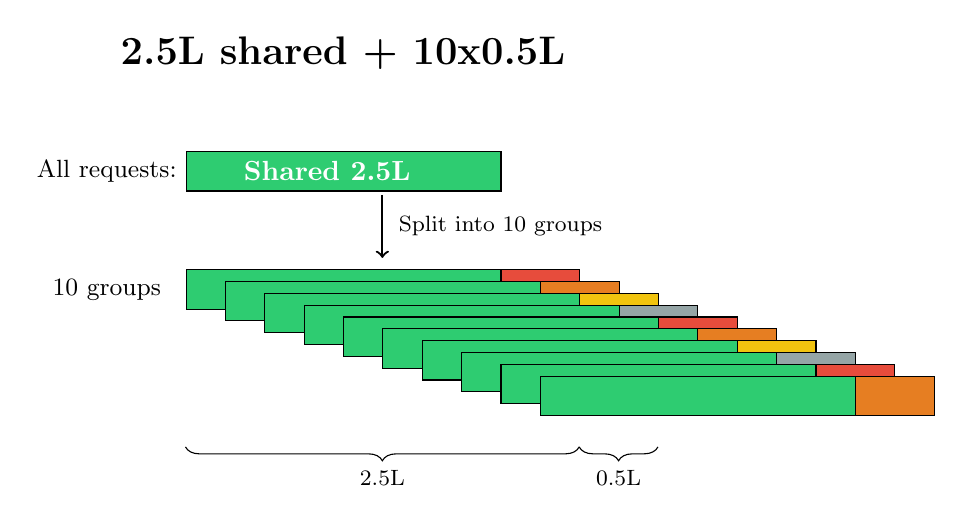
\begin{tikzpicture}[
    box/.style={rectangle, draw, minimum width=0.4cm, minimum height=0.5cm, anchor=west},
    label/.style={font=\small}
]
    \node[font=\Large\bfseries] at (5,4) {2.5L shared + 10x0.5L};
    
    \node[label] at (2,2.5) {All requests:};
    \node[box, fill=shared1, minimum width=4cm] at (3,2.5) {};
    \node[label, white, font=\bfseries] at (4.8,2.5) {Shared 2.5L};
    
    \node[label] at (2,1) {10 groups};
    
    \foreach \x/\col in {0/unique1, 1/unique2, 2/unique3, 3/unique4, 4/unique1, 5/unique2, 6/unique3, 7/unique4, 8/unique1, 9/unique2} {
        \node[box, fill=shared1, minimum width=4cm] at (3+\x*0.5,1-\x*0.15) {};
        \node[box, fill=\col, minimum width=1cm] at (7+\x*0.5,1-\x*0.15) {};
    }
    
    \draw[decorate, decoration={brace, amplitude=5pt, mirror}] 
        (3,-1.0) -- (8,-1.0) node[midway, below=5pt, font=\footnotesize] {2.5L};
    \draw[decorate, decoration={brace, amplitude=5pt, mirror}] 
        (8,-1.0) -- (9,-1.0) node[midway, below=5pt, font=\footnotesize] {0.5L};
    
    \draw[->, thick] (5.5,2.2) -- (5.5,1.4);
    \node[font=\footnotesize] at (7,1.8) {Split into 10 groups};
\end{tikzpicture}


{Mode 7}
    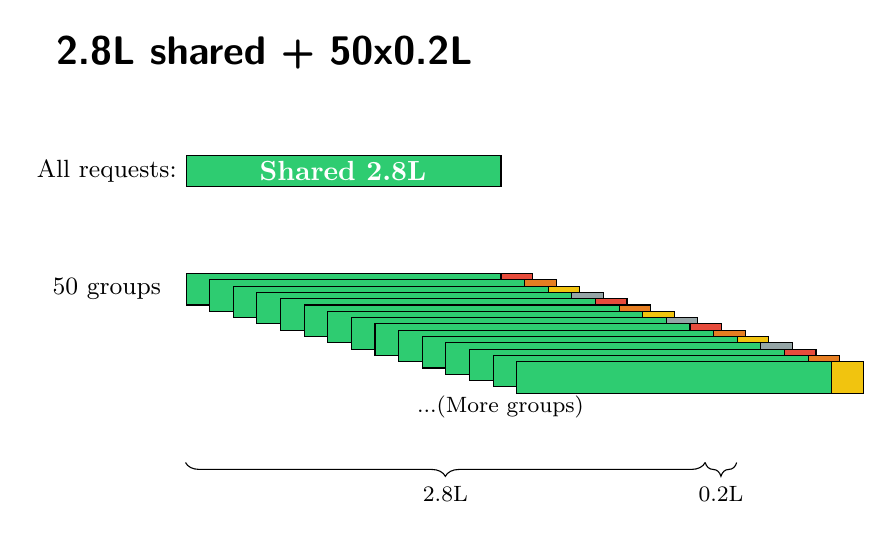
\begin{tikzpicture}[
    box/.style={rectangle, draw, minimum width=0.3cm, minimum height=0.4cm, anchor=west},
    label/.style={font=\small}
]
    \node[font=\Large\bfseries\sffamily] at (4,4) {2.8L shared + 50x0.2L};

    
    \node[label] at (2,2.5) {All requests:};
    \node[box, fill=shared1, minimum width=4cm] at (3,2.5) {};
    \node[label, white, font=\bfseries] at (5,2.5) {Shared 2.8L};
    \node[label] at (2,1) {50 groups};
    
    \foreach \x/\col in {0/unique1, 1/unique2, 2/unique3, 3/unique4, 4/unique1, 5/unique2, 6/unique3, 7/unique4, 8/unique1, 9/unique2, 10/unique3, 11/unique4, 12/unique1, 13/unique2, 14/unique3} {
        \node[box, fill=shared1, minimum width=4cm] at (3+\x*0.3,1-\x*0.08) {};
        \node[box, fill=\col, minimum width=0.4cm] at (7+\x*0.3,1-\x*0.08) {};
    }
    
    \node[font=\footnotesize] at (7,-0.5) {...(More groups)};
    
    \draw[decorate, decoration={brace, amplitude=5pt, mirror}] 
        (3,-1.2) -- (9.6,-1.2) node[midway, below=5pt, font=\footnotesize] {2.8L};
    \draw[decorate, decoration={brace, amplitude=5pt, mirror}] 
        (9.6,-1.2) -- (10,-1.2) node[midway, below=5pt, font=\footnotesize] {0.2L};
    
\end{tikzpicture}



{Mode 8}
    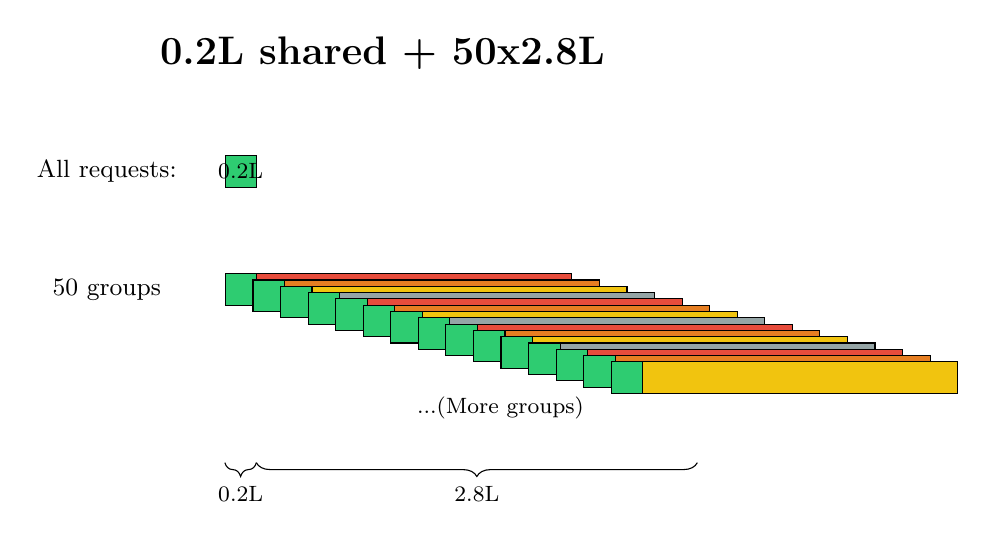
\begin{tikzpicture}[
    box/.style={rectangle, draw, minimum width=0.3cm, minimum height=0.4cm, anchor=west},
    label/.style={font=\small}
]
    \node[font=\Large\bfseries] at (5,4) {0.2L shared + 50x2.8L};
    
    \node[label] at (1.5,2.5) {All requests:};
    \node[box, fill=shared1, minimum width=0.4cm] at (3,2.5) {};
    \node[label, font=\footnotesize] at (3.2,2.5) {0.2L};
    
    \node[label] at (1.5,1) {50 groups};
    
    \foreach \x/\col in {0/unique1, 1/unique2, 2/unique3, 3/unique4, 4/unique1, 5/unique2, 6/unique3, 7/unique4, 8/unique1, 9/unique2, 10/unique3, 11/unique4, 12/unique1, 13/unique2, 14/unique3} {
        \node[box, fill=shared1, minimum width=0.4cm] at (3+\x*0.35,1-\x*0.08) {};
        \node[box, fill=\col, minimum width=4cm] at (3.4+\x*0.35,1-\x*0.08) {};
    }
    
    \node[font=\footnotesize] at (6.5,-0.5) {...(More groups)};
    
    \draw[decorate, decoration={brace, amplitude=5pt, mirror}] 
        (3,-1.2) -- (3.4,-1.2) node[midway, below=5pt, font=\footnotesize] {0.2L};
    \draw[decorate, decoration={brace, amplitude=5pt, mirror}] 
        (3.4,-1.2) -- (9,-1.2) node[midway, below=5pt, font=\footnotesize] {2.8L};
\end{tikzpicture}



{Comparison of Throughput across different modes}
\begin{table}[h!]
\centering
\begin{tabular}{|l|c|c|}
\hline
\textbf{Modes} & \textbf{L = 1000} & \textbf{L = 2000} \\
\hline
Mode 1 - All share 3L & 29.18 & 27.97 \\
Mode 2 - All share 2L, then 2xL & 19.94 & 14.06 \\
Mode 3 - All share L, then 2x2L& 15.40 & 8.89 \\
Mode 4 - L $\rightarrow$ 2L $\rightarrow$ 3L, 4 leaves& 15.41 & 9.88 \\
Mode 5 - 2 separate groups with 3L each & 10.18 & 6.62 \\
Mode 6 - 2.5L shared + 10x0.5L & 25.34 & 20.27 \\
Mode 7 - 2.8L shared + 50x0.2L & 28.05 & 23.17 \\
Mode 8 - 0.2L shared + 50x2.8L & 10.05 & 6.48 \\
\hline
\end{tabular}
\caption{Comparison of Throughput across different modes}
\end{table}



\section{Finding the Sweet Zone}
{How many families?}
\begin{itemize}
    \item A high request arrival rate (500 req/sec)
    \item Max batch size of 500
    \item A shared prefix of length 6500 tokens
    \item 100 new output tokens 
    \item Model: Llama3.1-8B
\end{itemize}
\begin{table}
\centering
\resizebox{\columnwidth}{!}{
\begin{tabular}{|c|cc|cc|}
\hline
\multirow{2}{*}{Number of Families} 
& \multicolumn{2}{c|}{vLLM Baseline (FCFS)} 
& \multicolumn{2}{c|}{vLLM (User-provided Family IDs)} \\
\cline{2-5}
& Average Batch Size & Throughput 
& Average Batch Size & Throughput \\
\hline
10  & 465.48  & 5.92 & 141.23 & 21.94 \\
20  & 455.47 & 5.74 & 72.67 & 15.27 \\
50  & 57.48 & 2.07 & 64.77 & 14.84 \\
100 & 41.97 & 1.11 & 67.14 & 14.82 \\
\hline
\end{tabular}
}
\end{table}



{How many req/sec?}
\begin{itemize}
    \item 5 families
    \item Max batch size of 500
    \item A shared prefix of length 6500 tokens
    \item 100 new output tokens 
    \item Model: Llama3.1-8B
\end{itemize}
\begin{table}
\centering
\resizebox{\columnwidth}{!}{
\begin{tabular}{|c|cc|cc|}
\hline
\multirow{2}{*}{req/sec} 
& \multicolumn{2}{c|}{vLLM Baseline (FCFS)} 
& \multicolumn{2}{c|}{vLLM (User-provided Family IDs)} \\
\cline{2-5}
& Average Batch Size & Throughput 
& Average Batch Size & Throughput \\
\hline
1  & 2.6  & 1.04 & 2.02 & 0.95 \\
2  & 5.15  & 2.00 & 4.48 & 1.99 \\
\rowcolor{lightgray}
5  & 29.60  & 5.09 & 11.11 & 4.40 \\
10  & 395.80  & 4.42 & 23.96 & 8.16 \\
20  & 438.85  & 5.25 & 52.79 & 13.32 \\
\hline
\end{tabular}
}
\end{table}



{How long should the shared prefix be?}
\begin{itemize}
    \item A high request arrival rate (500 req/sec)
    \item Max batch size of 500
    \item 5 families
    \item 100 new output tokens 
    \item Model: Llama3.1-8B
\end{itemize}
\begin{table}
\centering
\resizebox{\columnwidth}{!}{
\begin{tabular}{|c|cc|cc|}
\hline
\multirow{2}{*}{Shared Prefix Length in Number of Tokens} 
& \multicolumn{2}{c|}{vLLM Baseline (FCFS)} 
& \multicolumn{2}{c|}{vLLM (User-provided Family IDs)} \\
\cline{2-5}
& Average Batch Size & Throughput 
& Average Batch Size & Throughput \\
\hline
13  & 455.48 & 42.47 & 141.23 & 44.67 \\
\rowcolor{lightgray}
65  & 448.87  & 40.14 & 318.60 & 43.96 \\
130  & 460.09  & 38.19 & 330.49 & 41.99 \\
260  & 462.80  & 35.34 & 326.36 & 44.58 \\
650  & 469.12  & 27.47 & 335.21 & 42.00 \\
\hline
\end{tabular}
}
\end{table}


{How large should the model be?}
\begin{itemize}
    \item A high request arrival rate (500 req/sec)
    \item Max batch size of 500
    \item 5 families
    \item 100 new output tokens 
    \item Shared prefix length: 6500 tokens
\end{itemize}
\begin{table}
\centering
\resizebox{\columnwidth}{!}{
\begin{tabular}{|c|cc|cc|}
\hline
\multirow{2}{*}{Model Name} 
& \multicolumn{2}{c|}{vLLM Baseline (FCFS)} 
& \multicolumn{2}{c|}{vLLM (User-provided Family IDs)} \\
\cline{2-5}
& Average Batch Size & Throughput 
& Average Batch Size & Throughput \\
\hline
Qwen2.5-0.5B  & 378.98 & 25.40 & 89.63 & 49.08 \\
Llama3.1-8B  & 448.87  & 4.34 & 151.21 & 30.84 \\
LongChat-13B  & 5.28 & 0.61 & 215.70 & 22.01 \\
\hline
\end{tabular}
}
\end{table}


\section{Other experiments}

{Varying the amount of sharing}
\centering
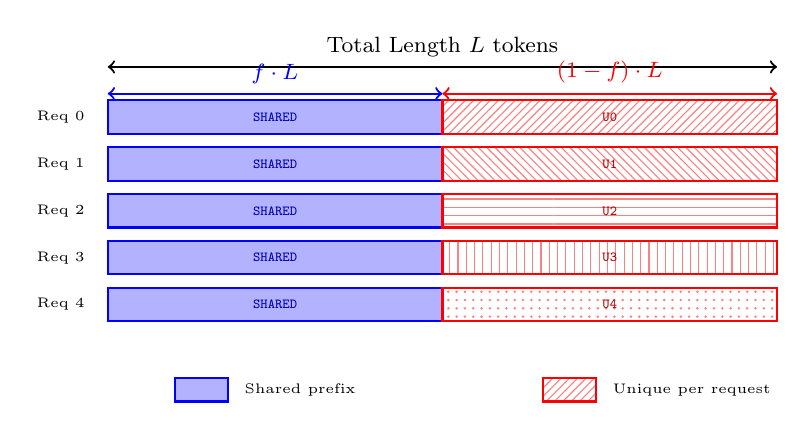
\begin{tikzpicture}[
    scale=0.85,
    every node/.style={font=\footnotesize}
]

\def\totalwidth{10}
\def\fraction{0.5} 
\pgfmathsetmacro{\sharedwidth}{\totalwidth * \fraction}
\pgfmathsetmacro{\uniquewidth}{\totalwidth * (1-\fraction)}
\def\boxheight{0.5}
\def\spacing{0.2}

\draw[<->, thick] (0, 2.2) -- (\totalwidth, 2.2) node[midway, above] {Total Length $L$ tokens};

\draw[<->, thick, blue] (0, 1.8) -- (\sharedwidth, 1.8) node[midway, above, blue] {$f \cdot L$};

\draw[<->, thick, red] (\sharedwidth, 1.8) -- (\totalwidth, 1.8) node[midway, above, red] {$(1-f) \cdot L$};

\foreach \i in {0,1,2,3,4} {
    \pgfmathsetmacro{\ypos}{1.2 - \i*(\boxheight + \spacing)}
    
    \fill[blue!30] (0, \ypos) rectangle (\sharedwidth, \ypos + \boxheight);
    \draw[thick, blue] (0, \ypos) rectangle (\sharedwidth, \ypos + \boxheight);
    
    \ifnum\i=0
        \fill[red!20, pattern=north east lines, pattern color=red!50] (\sharedwidth, \ypos) rectangle (\totalwidth, \ypos + \boxheight);
    \fi
    \ifnum\i=1
        \fill[red!20, pattern=north west lines, pattern color=red!50] (\sharedwidth, \ypos) rectangle (\totalwidth, \ypos + \boxheight);
    \fi
    \ifnum\i=2
        \fill[red!20, pattern=horizontal lines, pattern color=red!50] (\sharedwidth, \ypos) rectangle (\totalwidth, \ypos + \boxheight);
    \fi
    \ifnum\i=3
        \fill[red!20, pattern=vertical lines, pattern color=red!50] (\sharedwidth, \ypos) rectangle (\totalwidth, \ypos + \boxheight);
    \fi
    \ifnum\i=4
        \fill[red!20, pattern=dots, pattern color=red!50] (\sharedwidth, \ypos) rectangle (\totalwidth, \ypos + \boxheight);
    \fi
    \draw[thick, red] (\sharedwidth, \ypos) rectangle (\totalwidth, \ypos + \boxheight);
    
    \node[left, font=\tiny] at (-0.2, \ypos + \boxheight/2) {Req \i};
    
    \node[blue!70!black, font=\tiny] at (\sharedwidth/2, \ypos + \boxheight/2) {\texttt{SHARED}};
    \node[red!70!black, font=\tiny] at (\sharedwidth + \uniquewidth/2, \ypos + \boxheight/2) {\texttt{U\i}};
}


\fill[blue!30] (1, -2.8) rectangle ++(0.8, 0.35);
\draw[thick, blue] (1, -2.8) rectangle ++(0.8, 0.35);
\node[right, font=\tiny] at (1.9, -2.625) {Shared prefix};

\fill[red!20, pattern=north east lines, pattern color=red!50] (6.5, -2.8) rectangle ++(0.8, 0.35);
\draw[thick, red] (6.5, -2.8) rectangle ++(0.8, 0.35);
\node[right, font=\tiny] at (7.4, -2.625) {Unique per request};

\end{tikzpicture}

\vspace{0.3cm}


{Varying the amount of sharing (L = 100 tokens)}
    \begin{figure}
        \centering
    \includegraphics[width=\columnwidth]{\RESULTDIR/throughput_vs_amount_of_sharing_100.png}
    \captionof{figure}{Results across varying L}
\end{figure}


{Varying the amount of sharing (L = 500 tokens)}
    \begin{figure}
        \centering
    \includegraphics[width=\columnwidth]{\RESULTDIR/throughput_vs_amount_of_sharing_500.png}
    \captionof{figure}{Results across varying L}
\end{figure}


{Varying the amount of sharing (L = 1000 tokens)}
    \begin{figure}
        \centering
    \includegraphics[width=\columnwidth]{\RESULTDIR/throughput_vs_amount_of_sharing_1000.png}
    \captionof{figure}{Results across varying L}
\end{figure}


{Varying the amount of sharing (L = 2000 tokens)}
    \begin{figure}
        \centering
    \includegraphics[width=\columnwidth]{\RESULTDIR/throughput_vs_amount_of_sharing_2000.png}
    \captionof{figure}{Results across varying L}
\end{figure}


{Varying the amount of sharing (L = 500 tokens - More points)}
    \begin{figure}
        \centering
    \includegraphics[width=\columnwidth]{\RESULTDIR/throughput_vs_amount_of_sharing_500_more_points.png}
    \captionof{figure}{Results across varying L}
\end{figure}


{Two-family batch mixture}
\centering
\hspace*{-0.7cm}
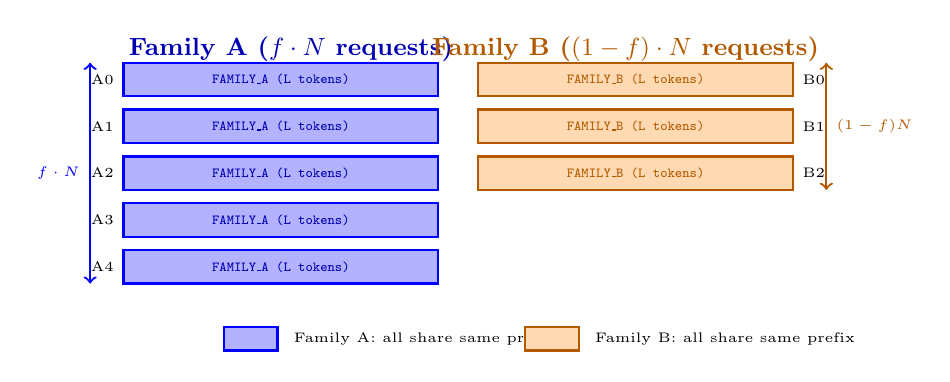
\begin{tikzpicture}[
    scale=0.85,
    every node/.style={font=\footnotesize}
]
% Parameters
\def\totalwidth{10}
\def\fraction{0.6}  % f = 0.6 (60% family A)
\pgfmathsetmacro{\halfwidth}{\totalwidth/2}
\pgfmathsetmacro{\leftwidth}{\halfwidth - 0.3}
\pgfmathsetmacro{\rightstart}{\halfwidth + 0.3}
\pgfmathsetmacro{\rightwidth}{\halfwidth - 0.3}
\def\boxheight{0.5}
\def\spacing{0.2}

% Title annotations
\node[font=\small\bfseries, blue!70!black] at (2.5, 2.5) {Family A ($f \cdot N$ requests)};
\node[font=\small\bfseries, orange!70!black] at (7.5, 2.5) {Family B ($(1-f) \cdot N$ requests)};

% Draw Family A requests
\foreach \i in {0,1,2,3,4} {
    \pgfmathsetmacro{\ypos}{1.8 - \i*(\boxheight + \spacing)}
    
    % Family A - all identical
    \fill[blue!30] (0, \ypos) rectangle (\leftwidth, \ypos + \boxheight);
    \draw[thick, blue] (0, \ypos) rectangle (\leftwidth, \ypos + \boxheight);
    
    % Label
    \node[left, font=\tiny] at (0, \ypos + \boxheight/2) {A\i};
    
    % Text inside
    \pgfmathsetmacro{\centerA}{\leftwidth/2}
    \node[blue!70!black, font=\tiny] at (\centerA, \ypos + \boxheight/2) {\texttt{FAMILY\_A (L tokens)}};
}

% Draw Family B requests
\foreach \i in {0,1,2} {
    \pgfmathsetmacro{\ypos}{1.8 - \i*(\boxheight + \spacing)}
    
    % Family B - all identical (but different from A)
    \fill[orange!30] (\rightstart, \ypos) rectangle (\totalwidth, \ypos + \boxheight);
    \draw[thick, orange!70!black] (\rightstart, \ypos) rectangle (\totalwidth, \ypos + \boxheight);
    
    % Label
    \node[right, font=\tiny] at (\totalwidth, \ypos + \boxheight/2) {B\i};
    
    % Text inside
    \pgfmathsetmacro{\centerB}{\rightstart + \rightwidth/2}
    \node[orange!70!black, font=\tiny] at (\centerB, \ypos + \boxheight/2) {\texttt{FAMILY\_B (L tokens)}};
}

% Annotations for counts
\pgfmathsetmacro{\topA}{1.8 + \boxheight}
\pgfmathsetmacro{\bottomA}{1.8 - 4*(\boxheight + \spacing)}
\draw[<->, thick, blue] (-0.5, \topA) -- (-0.5, \bottomA) 
    node[midway, left, font=\tiny] {$f \cdot N$};

\pgfmathsetmacro{\bottomB}{1.8 - 2*(\boxheight + \spacing)}    
\draw[<->, thick, orange!70!black] (\totalwidth + 0.5, \topA) -- (\totalwidth + 0.5, \bottomB) 
    node[midway, right, font=\tiny] {$(1-f) N$};

\fill[blue!30] (1.5, -2) rectangle ++(0.8, 0.35);
\draw[thick, blue] (1.5, -2) rectangle ++(0.8, 0.35);
\node[right, font=\tiny] at (2.4, -1.825) {Family A: all share same prefix};

\fill[orange!30] (6, -2) rectangle ++(0.8, 0.35);
\draw[thick, orange!70!black] (6, -2) rectangle ++(0.8, 0.35);
\node[right, font=\tiny] at (6.9, -1.825) {Family B: all share same prefix};

\end{tikzpicture}

\vspace{0.2cm}


{Two Family Batch Mixture (L = 100 tokens)}
    \begin{figure}
        \centering
    \includegraphics[width=\columnwidth]{\RESULTDIR/two_family_fraction_A_100.png}
    \captionof{figure}{Results across fraction of requests from A}
\end{figure}


{Two Family Batch Mixture (L = 500 tokens)}
    \begin{figure}
        \centering
    \includegraphics[width=\columnwidth]{\RESULTDIR/two_family_fraction_A_500.png}
    \captionof{figure}{Results across fraction of requests from A}
\end{figure}


{Two Family Batch Mixture (L = 1000 tokens)}
    \begin{figure}
        \centering
    \includegraphics[width=\columnwidth]{\RESULTDIR/two_family_fraction_A_1000.png}
    \captionof{figure}{Results across fraction of requests from A}
\end{figure}


{Two Family Batch Mixture (L = 2000 tokens)}
    \begin{figure}
        \centering
    \includegraphics[width=\columnwidth]{\RESULTDIR/two_family_fraction_A_2000.png}
    \captionof{figure}{Results across fraction of requests from A}
\end{figure}


{Tiered prefix sharing}
\centering
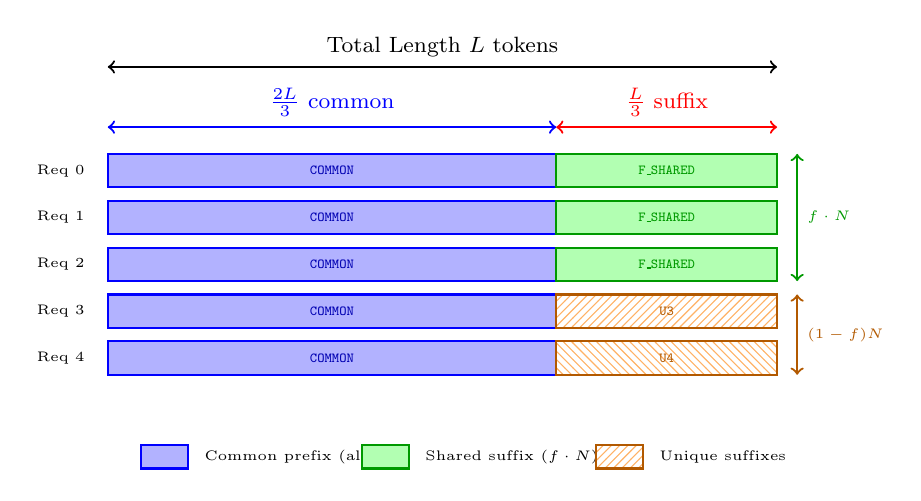
\begin{tikzpicture}[
    scale=0.85,
    every node/.style={font=\footnotesize}
]
% Parameters
\def\totalwidth{10}
\def\commonfrac{0.67}  % 2/3 of L is common
\pgfmathsetmacro{\commonwidth}{\totalwidth * \commonfrac}
\pgfmathsetmacro{\suffixwidth}{\totalwidth * (1-\commonfrac)}
\def\boxheight{0.5}
\def\spacing{0.2}
\def\fraction{0.6} 

\draw[<->, thick] (0, 2.7) -- (\totalwidth, 2.7) node[midway, above] {Total Length $L$ tokens};

\draw[<->, thick, blue] (0, 1.8) -- (\commonwidth, 1.8) node[midway, above, blue] {$\frac{2L}{3}$ common};


\draw[<->, thick, red] (\commonwidth, 1.8) -- (\totalwidth, 1.8) node[midway, above, red] {$\frac{L}{3}$ suffix};

\foreach \i in {0,1,2} {
    \pgfmathsetmacro{\ypos}{0.9 - \i*(\boxheight + \spacing)}
    
    \fill[blue!30] (0, \ypos) rectangle (\commonwidth, \ypos + \boxheight);
    \draw[thick, blue] (0, \ypos) rectangle (\commonwidth, \ypos + \boxheight);
    
    \fill[green!30] (\commonwidth, \ypos) rectangle (\totalwidth, \ypos + \boxheight);
    \draw[thick, green!60!black] (\commonwidth, \ypos) rectangle (\totalwidth, \ypos + \boxheight);
    
    \node[left, font=\tiny] at (-0.2, \ypos + \boxheight/2) {Req \i};
    
    \pgfmathsetmacro{\centerCommon}{\commonwidth/2}
    \pgfmathsetmacro{\centerSuffix}{\commonwidth + \suffixwidth/2}
    \node[blue!70!black, font=\tiny] at (\centerCommon, \ypos + \boxheight/2) {\texttt{COMMON}};
    \node[green!60!black, font=\tiny] at (\centerSuffix, \ypos + \boxheight/2) {\texttt{F\_SHARED}};
}

\foreach \i in {3,4} {
    \pgfmathsetmacro{\ypos}{0.9 - \i*(\boxheight + \spacing)}
    
    \fill[blue!30] (0, \ypos) rectangle (\commonwidth, \ypos + \boxheight);
    \draw[thick, blue] (0, \ypos) rectangle (\commonwidth, \ypos + \boxheight);
    
    \pgfmathsetmacro{\patternIdx}{int(\i-3)}
    \ifnum\patternIdx=0
        \fill[orange!20, pattern=north east lines, pattern color=orange!60] (\commonwidth, \ypos) rectangle (\totalwidth, \ypos + \boxheight);
    \fi
    \ifnum\patternIdx=1
        \fill[orange!20, pattern=north west lines, pattern color=orange!60] (\commonwidth, \ypos) rectangle (\totalwidth, \ypos + \boxheight);
    \fi
    \draw[thick, orange!70!black] (\commonwidth, \ypos) rectangle (\totalwidth, \ypos + \boxheight);
    
    \node[left, font=\tiny] at (-0.2, \ypos + \boxheight/2) {Req \i};
    
    \pgfmathsetmacro{\centerCommon}{\commonwidth/2}
    \pgfmathsetmacro{\centerSuffix}{\commonwidth + \suffixwidth/2}
    \node[blue!70!black, font=\tiny] at (\centerCommon, \ypos + \boxheight/2) {\texttt{COMMON}};
    \node[orange!70!black, font=\tiny] at (\centerSuffix, \ypos + \boxheight/2) {\texttt{U\i}};
}

\pgfmathsetmacro{\topShared}{0.9 + \boxheight}
\pgfmathsetmacro{\bottomShared}{0.9 - 2*(\boxheight + \spacing)}
\draw[<->, thick, green!60!black] (\totalwidth + 0.3, \topShared) -- (\totalwidth + 0.3, \bottomShared) 
    node[midway, right, font=\tiny] {$f \cdot N$};

\pgfmathsetmacro{\topUnique}{0.9 - 3*(\boxheight + \spacing) + \boxheight}
\pgfmathsetmacro{\bottomUnique}{0.9 - 4*(\boxheight + \spacing)}
\draw[<->, thick, orange!70!black] (\totalwidth + 0.3, \topUnique) -- (\totalwidth + 0.3, \bottomUnique) 
    node[midway, right, font=\tiny] {$(1-f) N$};


\fill[blue!30] (0.5, -3.3) rectangle ++(0.7, 0.35);
\draw[thick, blue] (0.5, -3.3) rectangle ++(0.7, 0.35);
\node[right, font=\tiny] at (1.3, -3.125) {Common prefix (all)};

\fill[green!30] (3.8, -3.3) rectangle ++(0.7, 0.35);
\draw[thick, green!60!black] (3.8, -3.3) rectangle ++(0.7, 0.35);
\node[right, font=\tiny] at (4.6, -3.125) {Shared suffix ($f \cdot N$)};

\fill[orange!20, pattern=north east lines, pattern color=orange!60] (7.3, -3.3) rectangle ++(0.7, 0.35);
\draw[thick, orange!70!black] (7.3, -3.3) rectangle ++(0.7, 0.35);
\node[right, font=\tiny] at (8.1, -3.125) {Unique suffixes};

\end{tikzpicture}

\vspace{0.2cm}


{Tiered Prefix Sharing (L = 500 tokens)}
    \begin{figure}
        \centering
    \includegraphics[width=\columnwidth]{\RESULTDIR/fraction_on_lower_tier_500.png}
    \captionof{figure}{Varying fraction on lowermost tier}
\end{figure}


{Tiered Prefix Sharing (L = 2000 tokens)}
    \begin{figure}
        \centering
    \includegraphics[width=\columnwidth]{\RESULTDIR/fraction_on_lower_tier_2000.png}
    \captionof{figure}{Varying fraction on lowermost tier}
\end{figure}



{Throughput vs Max Batch Size}
    \begin{figure}
        \centering
    \includegraphics[width=\columnwidth]{\RESULTDIR/throughput_vs_max_batch_size_1200.png}
    \captionof{figure}{Throughput vs Max Batch Size (L = 1200 tokens)}
\end{figure}


{Two Family Mixture - Mean DRAM Activity}
    \begin{figure}
        \centering
    \includegraphics[width=\columnwidth]{\RESULTDIR/mean_dram_act_frac_a_2000.png}
    \captionof{figure}{Mean DRAM Activity across fraction of requests from A (L = 2000 tokens)}
\end{figure}


{Two Family Mixture - Total DRAM Accesses}
    \begin{figure}
        \centering
    \includegraphics[width=\columnwidth]{\RESULTDIR/total_dram_acccesses_frac_a_2000.png}
    \captionof{figure}{Total DRAM Accesses across fraction of requests from A (L = 2000 tokens)}
\end{figure}



{Two Family Mixture - Mean SM Activity}
    \begin{figure}
        \centering
    \includegraphics[width=\columnwidth]{\RESULTDIR/sm_act_frac_a_2000.png}
    \captionof{figure}{Mean SM Activity across fraction of requests from A (L = 2000 tokens)}
\end{figure}


{Two Family Mixture - Mean SM Occupancy}
    \begin{figure}
        \centering
    \includegraphics[width=\columnwidth]{\RESULTDIR/sm_occ_frac_a_2000.png}
    \captionof{figure}{Mean SM Occupancy across fraction of requests from A (L = 2000 tokens)}
\end{figure}


{Two Family Mixture - Mean Tensor Core Utilization}
    \begin{figure}
        \centering
    \includegraphics[width=\columnwidth]{\RESULTDIR/tenso_frac_a_2000.png}
    \captionof{figure}{Mean Tensor Core Utilization across fraction of requests from A (L = 2000 tokens)}
\end{figure}




{Tiered Prefix Sharing}
\centering
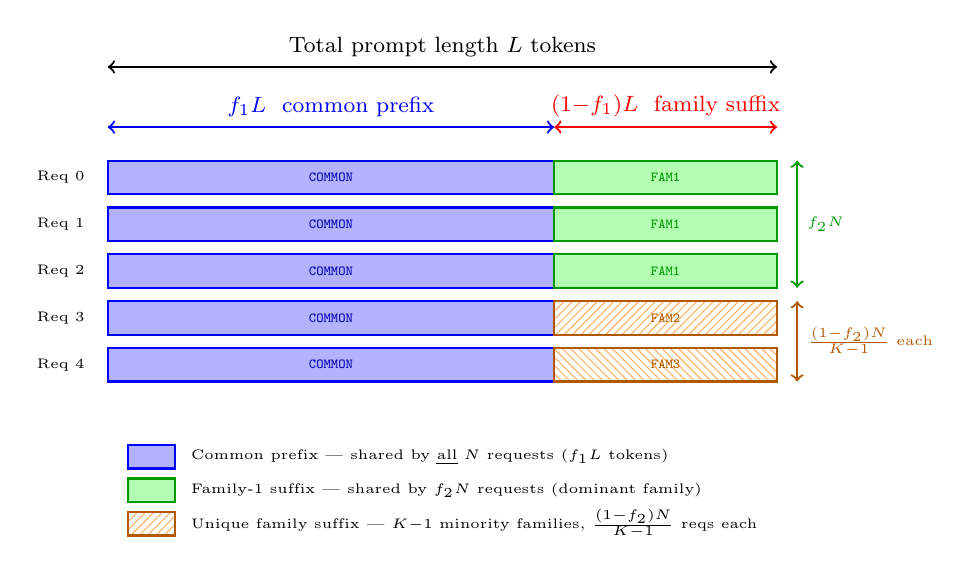
\begin{tikzpicture}[
    scale=0.85,
    every node/.style={font=\footnotesize}
]
% Parameters
\def\totalwidth{10}
\def\commonfrac{0.667}   % f1: fraction of L that is common prefix
\def\f{0.5}              % f2: fraction of N assigned to family 1
\def\numfamilies{6}      % total families (1 dominant + 5 others)
\pgfmathsetmacro{\commonwidth}{\totalwidth * \commonfrac}
\pgfmathsetmacro{\suffixwidth}{\totalwidth * (1-\commonfrac)}
\def\boxheight{0.5}
\def\spacing{0.2}

% ── top rulers ──────────────────────────────────────────────────────────────
\draw[<->, thick]
    (0, 2.8) -- (\totalwidth, 2.8)
    node[midway, above] {Total prompt length $L$ tokens};

\draw[<->, thick, blue]
    (0, 1.9) -- (\commonwidth, 1.9)
    node[midway, above, blue] {$f_1 L$ \ common prefix};

\draw[<->, thick, red]
    (\commonwidth, 1.9) -- (\totalwidth, 1.9)
    node[midway, above, red] {$(1{-}f_1)L$ \ family suffix};

% ── Family 1 rows (dominant family, f2*N requests) ───────────────────────
% We draw 3 representative rows
\foreach \i in {0,1,2} {
    \pgfmathsetmacro{\ypos}{0.9 - \i*(\boxheight + \spacing)}

    % Common prefix segment
    \fill[blue!30]  (0, \ypos) rectangle (\commonwidth, \ypos+\boxheight);
    \draw[thick, blue] (0, \ypos) rectangle (\commonwidth, \ypos+\boxheight);

    % Family-1 shared suffix
    \fill[green!30] (\commonwidth, \ypos) rectangle (\totalwidth, \ypos+\boxheight);
    \draw[thick, green!60!black] (\commonwidth, \ypos) rectangle (\totalwidth, \ypos+\boxheight);

    \node[left, font=\tiny] at (-0.2, \ypos+\boxheight/2) {Req \i};
    \pgfmathsetmacro{\cx}{\commonwidth/2}
    \pgfmathsetmacro{\sx}{\commonwidth + \suffixwidth/2}
    \node[blue!70!black,  font=\tiny] at (\cx, \ypos+\boxheight/2) {\texttt{COMMON}};
    \node[green!60!black, font=\tiny] at (\sx, \ypos+\boxheight/2) {\texttt{FAM1}};
}

% ── Other-family rows (5 families, each with unique suffix) ──────────────
% We draw 2 representative rows (one per other family shown)
\foreach \i in {3,4} {
    \pgfmathsetmacro{\ypos}{0.9 - \i*(\boxheight + \spacing)}
    \pgfmathsetmacro{\famnum}{int(\i-1)}   % FAM2, FAM3, ...

    % Common prefix segment
    \fill[blue!30]  (0, \ypos) rectangle (\commonwidth, \ypos+\boxheight);
    \draw[thick, blue] (0, \ypos) rectangle (\commonwidth, \ypos+\boxheight);

    % Unique suffix (hatched orange, different pattern per row)
    \pgfmathsetmacro{\patternIdx}{int(\i-3)}
    \ifnum\patternIdx=0
        \fill[orange!20, pattern=north east lines, pattern color=orange!60]
            (\commonwidth, \ypos) rectangle (\totalwidth, \ypos+\boxheight);
    \fi
    \ifnum\patternIdx=1
        \fill[orange!20, pattern=north west lines, pattern color=orange!60]
            (\commonwidth, \ypos) rectangle (\totalwidth, \ypos+\boxheight);
    \fi
    \draw[thick, orange!70!black] (\commonwidth, \ypos) rectangle (\totalwidth, \ypos+\boxheight);

    \node[left, font=\tiny] at (-0.2, \ypos+\boxheight/2) {Req \i};
    \pgfmathsetmacro{\cx}{\commonwidth/2}
    \pgfmathsetmacro{\sx}{\commonwidth + \suffixwidth/2}
    \node[blue!70!black,   font=\tiny] at (\cx, \ypos+\boxheight/2) {\texttt{COMMON}};
    \node[orange!70!black, font=\tiny] at (\sx, \ypos+\boxheight/2) {\texttt{FAM\famnum}};
}

% ── Right-side braces showing request counts ─────────────────────────────
% Family-1 brace  (rows 0..2)
\pgfmathsetmacro{\topF}{0.9 + \boxheight}
\pgfmathsetmacro{\botF}{0.9 - 2*(\boxheight + \spacing)}
\draw[<->, thick, green!60!black]
    (\totalwidth+0.3, \topF) -- (\totalwidth+0.3, \botF)
    node[midway, right, font=\tiny] {$f_2 N$};

% Other-families brace  (rows 3..4)
\pgfmathsetmacro{\topO}{0.9 - 3*(\boxheight+\spacing) + \boxheight}
\pgfmathsetmacro{\botO}{0.9 - 4*(\boxheight+\spacing)}
\draw[<->, thick, orange!70!black]
    (\totalwidth+0.3, \topO) -- (\totalwidth+0.3, \botO)
    node[midway, right, font=\tiny]
    {$\frac{(1{-}f_2)N}{K{-}1}$ each};

% ── Legend ───────────────────────────────────────────────────────────────
\fill[blue!30]   (0.3,-3.2) rectangle ++(0.7,0.35);
\draw[thick,blue](0.3,-3.2) rectangle ++(0.7,0.35);
\node[right, font=\tiny] at (1.1,-3.025)
    {Common prefix — shared by \emph{all} $N$ requests ($f_1 L$ tokens)};

\fill[green!30]  (0.3,-3.7) rectangle ++(0.7,0.35);
\draw[thick,green!60!black](0.3,-3.7) rectangle ++(0.7,0.35);
\node[right, font=\tiny] at (1.1,-3.525)
    {Family-1 suffix — shared by $f_2 N$ requests (dominant family)};

\fill[orange!20, pattern=north east lines, pattern color=orange!60]
    (0.3,-4.2) rectangle ++(0.7,0.35);
\draw[thick,orange!70!black](0.3,-4.2) rectangle ++(0.7,0.35);
\node[right, font=\tiny] at (1.1,-4.025)
    {Unique family suffix — $K{-}1$ minority families, $\frac{(1-f_2)N}{K-1}$ reqs each};

\end{tikzpicture}
\vspace{0.2cm}


{Tiered Prefix Sharing (L = 2000 tokens) (Number of families = 6)}
    \begin{figure}
        \centering
    \includegraphics[width=\columnwidth]{\RESULTDIR/tiered_prefix_sharing_2000_fam_6_f1_f2.png}
\end{figure}


{Tiered Prefix Sharing (L = 10000 tokens) (Number of families = 6)}
    \begin{figure}
        \centering
    \includegraphics[width=\columnwidth]{\RESULTDIR/tiered_prefix_sharing_10000_fam_6_f1_f2.png}
\end{figure}


{Tiered Prefix Sharing (L = 2000 tokens) (Number of families = 51)}
    \begin{figure}
        \centering
    \includegraphics[width=\columnwidth]{\RESULTDIR/tiered_prefix_sharing_2000_fam_51_f1_f2.png}
\end{figure}


{Tiered Prefix Sharing (L = 10000 tokens) (Number of families = 51)}
    \begin{figure}
        \centering
    \includegraphics[width=\columnwidth]{\RESULTDIR/tiered_prefix_sharing_10000_fam_51_f1_f2.png}
\end{figure}


{Varying the amount of sharing}
\centering
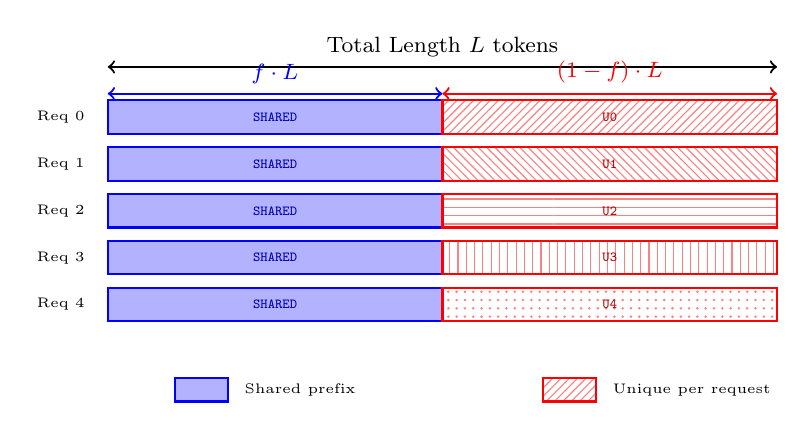
\begin{tikzpicture}[
    scale=0.85,
    every node/.style={font=\footnotesize}
]

\def\totalwidth{10}
\def\fraction{0.5} 
\pgfmathsetmacro{\sharedwidth}{\totalwidth * \fraction}
\pgfmathsetmacro{\uniquewidth}{\totalwidth * (1-\fraction)}
\def\boxheight{0.5}
\def\spacing{0.2}

\draw[<->, thick] (0, 2.2) -- (\totalwidth, 2.2) node[midway, above] {Total Length $L$ tokens};

\draw[<->, thick, blue] (0, 1.8) -- (\sharedwidth, 1.8) node[midway, above, blue] {$f \cdot L$};

\draw[<->, thick, red] (\sharedwidth, 1.8) -- (\totalwidth, 1.8) node[midway, above, red] {$(1-f) \cdot L$};

\foreach \i in {0,1,2,3,4} {
    \pgfmathsetmacro{\ypos}{1.2 - \i*(\boxheight + \spacing)}
    
    \fill[blue!30] (0, \ypos) rectangle (\sharedwidth, \ypos + \boxheight);
    \draw[thick, blue] (0, \ypos) rectangle (\sharedwidth, \ypos + \boxheight);
    
    \ifnum\i=0
        \fill[red!20, pattern=north east lines, pattern color=red!50] (\sharedwidth, \ypos) rectangle (\totalwidth, \ypos + \boxheight);
    \fi
    \ifnum\i=1
        \fill[red!20, pattern=north west lines, pattern color=red!50] (\sharedwidth, \ypos) rectangle (\totalwidth, \ypos + \boxheight);
    \fi
    \ifnum\i=2
        \fill[red!20, pattern=horizontal lines, pattern color=red!50] (\sharedwidth, \ypos) rectangle (\totalwidth, \ypos + \boxheight);
    \fi
    \ifnum\i=3
        \fill[red!20, pattern=vertical lines, pattern color=red!50] (\sharedwidth, \ypos) rectangle (\totalwidth, \ypos + \boxheight);
    \fi
    \ifnum\i=4
        \fill[red!20, pattern=dots, pattern color=red!50] (\sharedwidth, \ypos) rectangle (\totalwidth, \ypos + \boxheight);
    \fi
    \draw[thick, red] (\sharedwidth, \ypos) rectangle (\totalwidth, \ypos + \boxheight);
    
    \node[left, font=\tiny] at (-0.2, \ypos + \boxheight/2) {Req \i};
    
    \node[blue!70!black, font=\tiny] at (\sharedwidth/2, \ypos + \boxheight/2) {\texttt{SHARED}};
    \node[red!70!black, font=\tiny] at (\sharedwidth + \uniquewidth/2, \ypos + \boxheight/2) {\texttt{U\i}};
}


\fill[blue!30] (1, -2.8) rectangle ++(0.8, 0.35);
\draw[thick, blue] (1, -2.8) rectangle ++(0.8, 0.35);
\node[right, font=\tiny] at (1.9, -2.625) {Shared prefix};

\fill[red!20, pattern=north east lines, pattern color=red!50] (6.5, -2.8) rectangle ++(0.8, 0.35);
\draw[thick, red] (6.5, -2.8) rectangle ++(0.8, 0.35);
\node[right, font=\tiny] at (7.4, -2.625) {Unique per request};

\end{tikzpicture}

\vspace{0.3cm}



{Varying the amount of sharing - different RL Techniques}
    \begin{figure}
        \centering
    \includegraphics[width=\columnwidth]{\RESULTDIR/fraction_sharing_throughput_average_batch_size.png}
    \captionof{figure}{Throughput and Average Batch Sizes across Fractions ($L = 1200$ tokens, batch of $100$ requests)}
\end{figure}


{Varying the amount of sharing - different RL Techniques - average batch size (fraction = 0)}
    \begin{figure}
        \centering
    \includegraphics[width=\columnwidth]{\RESULTDIR/fraction_sharing_policies_0.png}
\end{figure}


{Varying the amount of sharing - different RL Techniques - average batch size (fraction = 0.2)}
    \begin{figure}
        \centering
    \includegraphics[width=\columnwidth]{\RESULTDIR/fraction_sharing_policies_0.2.png}
\end{figure}



{Varying the amount of sharing - different RL Techniques - average batch size (fraction = 0.4)}
    \begin{figure}
        \centering
    \includegraphics[width=\columnwidth]{\RESULTDIR/fraction_sharing_policies_0.4.png}
\end{figure}



{Varying the amount of sharing - different RL Techniques - average batch size (fraction = 0.6)}
    \begin{figure}
        \centering
    \includegraphics[width=\columnwidth]{\RESULTDIR/fraction_sharing_policies_0.6.png}
\end{figure}



{Varying the amount of sharing - different RL Techniques - average batch size (fraction = 0.8)}
    \begin{figure}
        \centering
    \includegraphics[width=\columnwidth]{\RESULTDIR/fraction_sharing_policies_0.8.png}
\end{figure}



{Varying the amount of sharing - different RL Techniques - average batch size (fraction = 1.0)}
    \begin{figure}
        \centering
    \includegraphics[width=\columnwidth]{\RESULTDIR/fraction_sharing_policies_1.0.png}
\end{figure}

\end{document}